%\documentclass[3p,times,procedia,number]{elsarticle}
\documentclass[3p,times,number,review]{elsarticle}
\usepackage{lineno}
\modulolinenumbers[5]

\flushbottom

%% The `ecrc' package must be called to make the CRC functionality available
\usepackage{ecrc}
\usepackage{amsmath}
\usepackage{cases}
\usepackage{amssymb}
\usepackage{mathtools}
\usepackage{bm}
\usepackage{verbatim}
%\usepackage[fleqn]{amsmath}
\usepackage{caption}
\usepackage{ulem}
\usepackage[colorlinks,linkcolor=blue,citecolor=blue,urlcolor=blue]{hyperref}
\usepackage{graphicx} 
\usepackage[subfigure]{graphfig}
\setcounter{totalnumber}{4}
\renewcommand{\textfraction}{0.15}
\renewcommand{\topfraction}{0.85}
\renewcommand{\bottomfraction}{0.65}
\renewcommand{\floatpagefraction}{0.60}
\newcommand{\figref}[1]{\figurename~\ref{#1}}
\usepackage{titlesec}
\titleformat{\chapter}[display]
{\normalfont\Large\bfseries}{\thechapter}{11pt}{\Large}
\titleformat{\section}
{\normalfont\large\bfseries}{\thesection}{11pt}{\large}
\titlespacing*{\chapter}{0pt}{0pt}{15pt} %left, beforesep, aftersep, right
\titlespacing*{\section}{0pt}{3.5ex plus 1ex minus .2ex}{2.3ex plus .2ex}
\usepackage[titletoc]{appendix}
\usepackage{listings}
\makeatletter
\newcommand{\rmnum}[1]{\romannumeral #1}
\newcommand{\Rmnum}[1]{\expandafter\@slowromancap\romannumeral #1@}
\makeatother
\newcommand{\HRule}{\rule{\linewidth}{0.5mm}}
\usepackage{xltxtra}
%\usepackage[francais]{babel}
\usepackage{listings}
\lstset{language=Matlab}%code language matlab
\lstset{breaklines}% long code break line
\lstset{extendedchars=false}
%\usepackage[framed,numbered,autolinebreaks,useliterate]{mcode}
\usepackage[table,xcdraw]{xcolor}
\usepackage{datetime}
\usepackage{multirow,tabularx}
\usepackage{bbm}
\usepackage{amsmath}
\DeclareMathOperator{\Tr}{Tr}
%% The ecrc package defines commands needed for running heads and logos.
%% For running heads, you can set the journal name, the volume, the starting page and the authors

%% set the volume if you know. Otherwise `00'
\volume{00}

%% set the starting page if not 1
\firstpage{1}

%% Give the name of the journal
\journalname{International Journal of Fatigue}

%% Give the author list to appear in the running head
%% Example \runauth{C.V. Radhakrishnan et al.}
\runauth{Ma Zepeng et al.}

%% The choice of journal logo is determined by the \jid and \jnltitlelogo commands.
%% A user-supplied logo with the name <\jid>logo.pdf will be inserted if present.
%% e.g. if \jid{yspmi} the system will look for a file yspmilogo.pdf
%% Otherwise the content of \jnltitlelogo will be set between horizontal lines as a default logo

%% Give the abbreviation of the Journal.
\jid{proeng}

%% Give a short journal name for the dummy logo (if needed)
%\jnltitlelogo{Procedia Engineering}

%% Hereafter the template follows `elsarticle'.
%% For more details see the existing template files elsarticle-template-harv.tex and elsarticle-template-num.tex.

%% Elsevier CRC generally uses a numbered reference style
%% For this, the conventions of elsarticle-template-num.tex should be followed (included below)
%% If using BibTeX, use the style file elsarticle-num.bst

%% End of ecrc-specific commands
%%%%%%%%%%%%%%%%%%%%%%%%%%%%%%%%%%%%%%%%%%%%%%%%%%%%%%%%%%%%%%%%%%%%%%%%%%

%% The amssymb package provides various useful mathematical syméls

\usepackage{amssymb}
%% The amsthm package provides extended theorem environments
%% \usepackage{amsthm}

%% The lineno packages adds line numbers. Start line numbering with
%% \begin{linenumbers}, end it with \end{linenumbers}. Or switch it on
%% for the whole article with \linenumbers after \end{frontmatter}.
%% \usepackage{lineno}

%% natbib.sty is loaded by default. However, natbib options can be
%% provided with \biboptions{...} command. Following options are
%% valid:

%%   round  -  round parentheses are used (default)
%%   square -  square brackets are used   [option]
%%   curly  -  curly braces are used      {option}
%%   angle  -  angle brackets are used    <option>
%%   semicolon  -  multiple citations separated by semi-colon
%%   colon  - same as semicolon, an earlier confusion
%%   comma  -  separated by comma
%%   numbers-  selects numerical citations
%%   super  -  numerical citations as superscripts
%%   sort   -  sorts multiple citations according to order in ref. list
%%   sort&compress   -  like sort, but also compresses numerical citations
%%   compress - compresses without sorting
%%
%\biboptions{authoryear}
\bibliographystyle{elsarticle-num}
 \biboptions{sort&compress}

% if you have landscape tables
\usepackage[figuresright]{rotating}
%\usepackage{harvard}
% put your own definitions here:x
%   \newcommand{\cZ}{\cal{Z}}
%   \newtheorem{def}{Definition}[section]
%   ...

% add words to TeX's hyphenation exception list
%\hyphenation{author another created financial paper re-commend-ed Post-Script}

% declarations for front matter

\begin{document}

\begin{frontmatter}

%% Title, authors and addresses

%% use the tnoteref command within \title for footnotes;
%% use the tnotetext command for the associated footnote;
%% use the fnref command within \author or \address for footnotes;
%% use the fntext command for the associated footnote;
%% use the corref command within \author for corresponding author footnotes;
%% use the cortext command for the associated footnote;
%% use the ead command for the email address,
%% and the form \ead[url] for the home page:
%%
%% \title{Title\tnoteref{label1}}
%% \tnotetext[label1]{}
%% \author{Name\corref{cor1}\fnref{label2}}
%% \ead{email address}
%% \ead[url]{home page}
%% \fntext[label2]{}
%% \cortext[cor1]{}
%% \address{Address\fnref{label3}}
%% \fntext[label3]{}
%\dochead{International Conference on Fatigue Damage of Structural Materials XI}
%\dochead{1st year PhD research result}
%% Use \dochead if there is an article header, e.g. \dochead{Short communication}
%% \dochead can also be used to include a conference title, if directed by the editors
%% e.g. \dochead{17th International Conference on Dynamical Processes in Excited States of Solids}

\title{A new strategy for fatigue analysis in presence of general multiaxial time varying loadings}

%% use optional labels to link authors explicitly to addresses:
%% \author[label1,label2]{<author name>}
%% \address[label1]{<address>}
%% \address[label2]{<address>}



\author[a]{Ma Zepeng\corref{cor1}}
\author[b]{Patrick Le Tallec}
\author[c]{Habibou Maitournam}

\address[a]{Laboratory of Solid Mechanics, Ecole Polytechnique, 91128 Palaiseau Cedex, France}
\address[b]{Laboratory of Solid Mechanics, Ecole Polytechnique, 91128 Palaiseau Cedex, France}
\address[c]{IMSIA, ENSTA ParisTech, CNRS, CEA, EDF, Université Paris-Saclay, 828 bd des Maréchaux, 91762 Palaiseau cedex France}

\begin{abstract}
%% Text of abstract
The object of this paper is to propose an energy based fatigue approach which handles multidimensional time varying loading histories.

Our fundamental thought is to assume that the energy dissipated at small scales governs fatigue at failure. The basis of our model is to consider a plastic behavior at the mesoscopic scale with a dependence of the yield function not only on the deviatoric part of the stress but also on the hydrostatic part. A kinematic hardening under the assumption of associative plasticity is also considered. We also follow the Dang Van paradigm at macro scale. The structure is elastic at the macroscopic scale. At each material points, there is a stochastic distribution of weak points which will undergo strong plastic yielding, which contribute to energy dissipation without affecting the overall macroscopic stress.

Instead of using the number of cycles, we use the concept of loading history. To accommodate real life loading history more accurately, mean stress effect is taken into account in mesoscopic yield function and non-linear damage accumulation law are also considered in our model. Fatigue will then be determined from the plastic shakedown cycle and from a phenomenological fatigue law linking lifetime and accumulated mesoscopic plastic dissipation.
 
\end{abstract}

\begin{keyword}
Fatigue; Energy; High cycle; Plasticity; Mean stress

%% keywords here, in the form: keyword \sep keyword

%% PACS codes here, in the form: \PACS code \sep code

%% MSC codes here, in the form: \MSC code \sep code
%% or \MSC[2008] code \sep code (2000 is the default)

\end{keyword}

\cortext[cor1]{Corresponding author. Email address: zepeng.ma@polytechnique.edu }

\end{frontmatter}

\clearpage
\begin{flushleft}
	\textbf{Nomenclature}
	\vspace{6pt}
	\begin{table}[h]
		\begin{tabular}{lllll}
			$S_{max}$ & maximum deviatoric stress during the loading cycles &  &  &  \\
		    $\sigma_{-1}$ & fatigue limit for fully reversed condition  &  &  &  \\
			$b$ & back stress  &  &  &  \\
			$\dot{w}$ & energy dissipation rate at a certain scale &  &  &  \\
			$\dot{W}$ & energy dissipation rate at all scales &  &  &  \\
			$W$ & dissipated energy&  &  &  \\
			$W_{cyc}$ & dissipated energy per cycle &  &  &  \\
			$N$& current number of cycles &  &  &  \\
			$N_F$& number of cycles to failure &  &  &  \\
			 $ \dot{\varepsilon}_p$ & rate of effective plastic strain &  &  &  \\
			$W_0$ & dissipated energy to failure per unit volume &  &  &  \\
			$E$ & Young's modulus &  &  &  \\
			$k=500\sim800MPa$ & hardening parameter &  &  &  \\
			$\beta=1\sim50$ & weakening scales distribution exponent  &  &  &  \\
			$\gamma=0\sim50$ & material parameter from Chaboche law(Wohler curve exponent)  &  &  &  \\
			$\alpha=1 - a\left\langle \dfrac{\dfrac{1}{2}\sigma_{vm}(t)-\sigma_{-1}\left(1-3c\sigma_{H,max}(t) \right) }{\sigma_{u} -\sigma_{vm}(t)}\right\rangle$ & characterizes non-linearity of damage accumulation(c is constant) &  &  &  \\
			$a$ & material parameter from Chaboche law &  &  &  \\
			$M_0 $ & material parameter in Chaboche law &  &  &  \\
			$\sigma_{y}$ & macroscopic yield stress(normal or shear) &  &  &  \\
			$\lambda=0\sim5$& hydrostatic pressure sensitivity &  &  &  \\
			$\uline{\uline{S}}=dev\dot{\uline{\uline{\Sigma}}}$ & deviatoric part of the stress tensor &  &  &  \\
			$\Sigma_H$& macroscopic hydrostatic pressure &  &  &  \\
			$A_{\uppercase\expandafter{\romannumeral2}}=\tau_{oct,a}=\sqrt{\dfrac{1}{3}J_{2,a}}$& the amplitude of octahedral shear stress &  &  &  \\
			$S_{max}=\sigma_{VM}=\sqrt{6J_{2,a}}$& Von Mises stress &  &  &  \\
			$s_{-1}$& tensile fatigue limit for $R=-1$  &  &  &  \\
			$\langle$ $\rangle$& Macaulay bracket symbol.$\langle$ $\rangle$ is defined as $\langle m\rangle=0$ if $m\leqslant0$
	\end{tabular}
	\end{table}
\end{flushleft}

\clearpage

\section{Weakening scales and yield function}
\subsection{The concept of weakening scales} 

We follow the Dang Van paradigm. The structure is elastic at the macroscopic scale. At each material points, there is a stochastic distribution of weak points which will undergo strong plastic yielding, without contributing to the overall macroscopic stress. From a microscopic point of view, there is a distribution of weakening scales, namely $s\in[1,\infty)$. Let $S_{max}$ be the macroscopic stress intensity at present time. Let $\sigma_y$ be the yield limit before weakening. Then we imagine that for a given scale $s$:

\vspace{6pt}
\noindent
$\bullet$ either $1\leqslant s\leqslant \sigma_y/S_{max}$, then $S_{max}\leqslant \sigma_y/s$, the material stays in the elastic regime and there is no energy dissipation at this scale.

\vspace{6pt}
\noindent
$\bullet$ or $\sigma_y/S_{max}\leqslant s\leqslant \infty$, then $S_{max}\geqslant \sigma_y/s$, the material is in the plastic regime and there is dissipated energy at scale $s$, contributing to the fatigue limit, which evolve through kinematic hardening.

In more details, at each scale $s$ of a plastic evolution process there is a weakened yield limit $\sigma_y/s$, zero initial plastic strain $\uuline{\varepsilon}_p$ and zero initial backstress $\uuline{b}$ at initial time $t_0$.


\vspace{6pt}

\subsection{Distribution of weakening scales}

We assume the weakening scales have a  probability distribution function of power law:
$$P(s) = Hs^{-\beta},$$

where $\beta$ is a material constant and $H$ is hardening constant. 
The choice of a power law has two reasons: on one hand, this type of distribution corresponds to a scale invariant process, on the other hand it leads in cyclic loading to a prediction of a number of cycles to life limit as a power law function of the stress intensity. More general laws can also be proposed.

The integrated probability ranging from macroscopic to microscopic stress  is unity. From this we can conclude:
$$\int_{1}^{\infty}P(s)ds=\left[ \frac{Hs^{1-\beta}}{1-\beta}\right] _{1}^{\infty}=0-\frac{H}{1-\beta}=1.$$


Then we know $H=\beta-1$, so the distribution is given by:
$$P(s) = Hs^{-\beta}=(\beta-1)s^{-\beta}$$
The probability of weakening scales is shown in \figref{ps1} and \figref{ps2}. We can see smaller $\beta$ has larger probability of weakening.
\begin{figure}[!h]
	\centering
	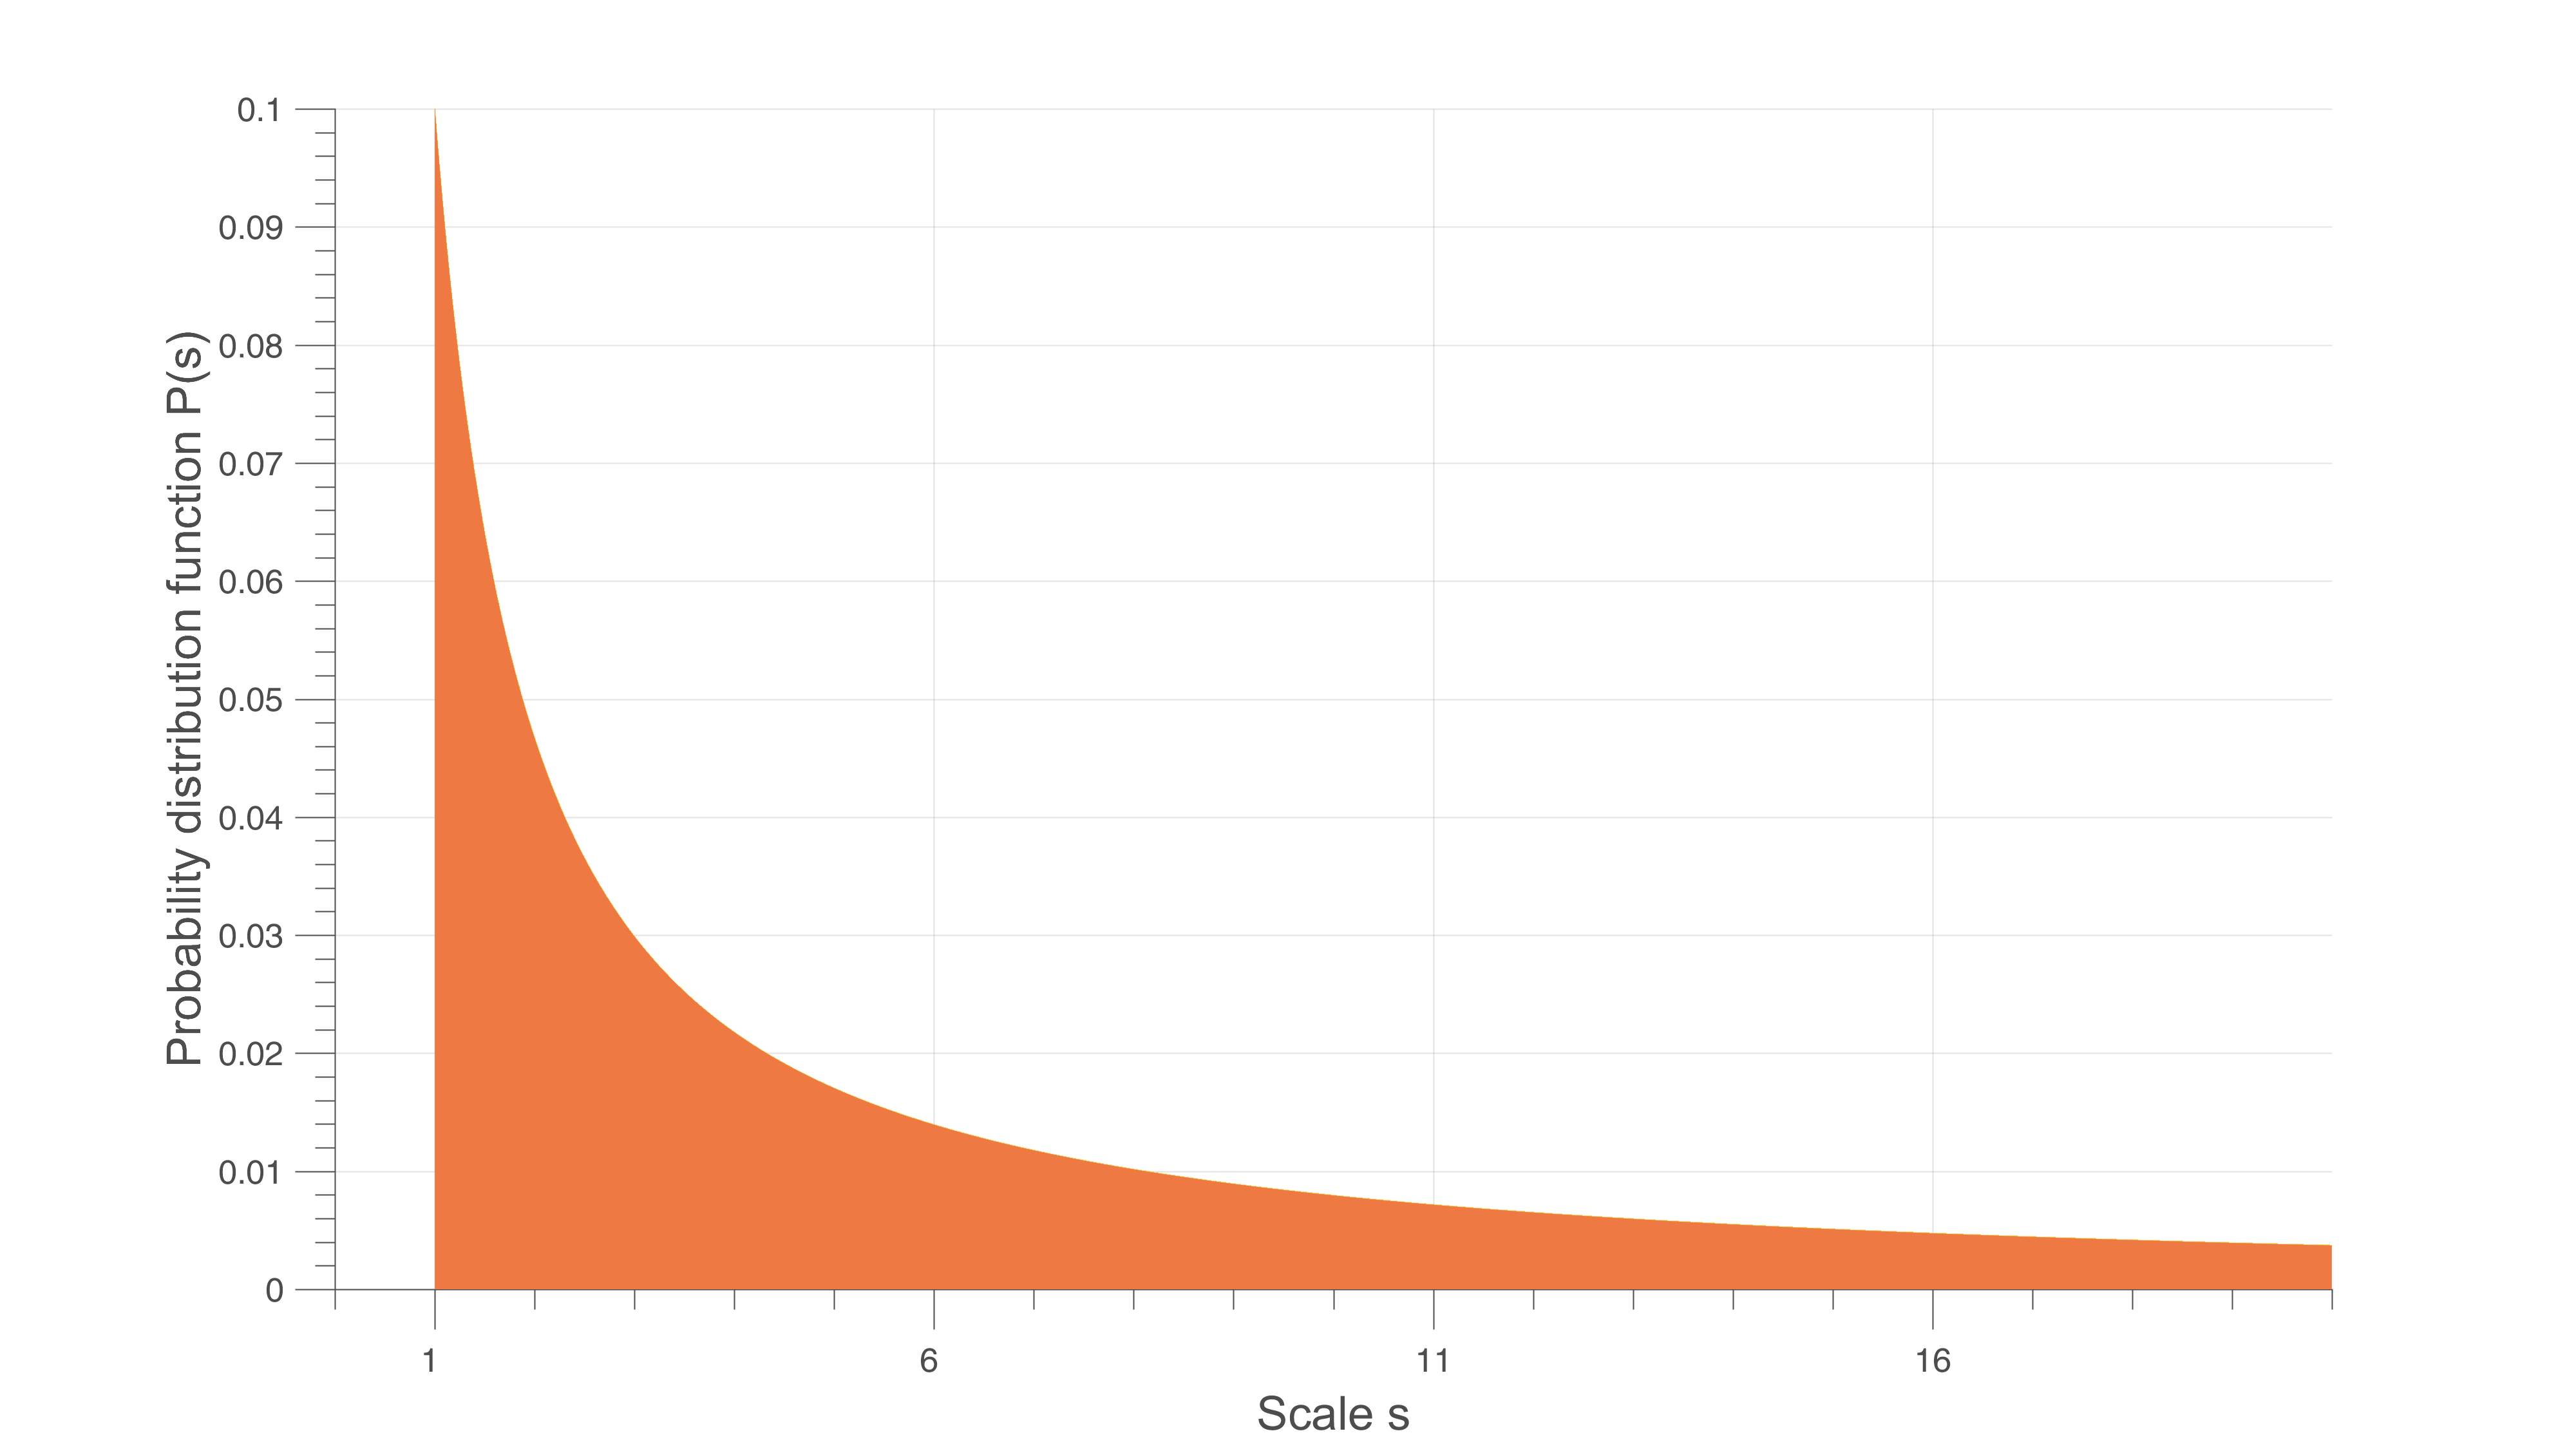
\includegraphics[width=0.9\textwidth]{figures//ps1.png} 
	\caption{Weakening scales $s$ probability distribution curve when $\beta=1.5$ }
	\label{ps1}
\end{figure}
\begin{figure}[!h]
	\centering
	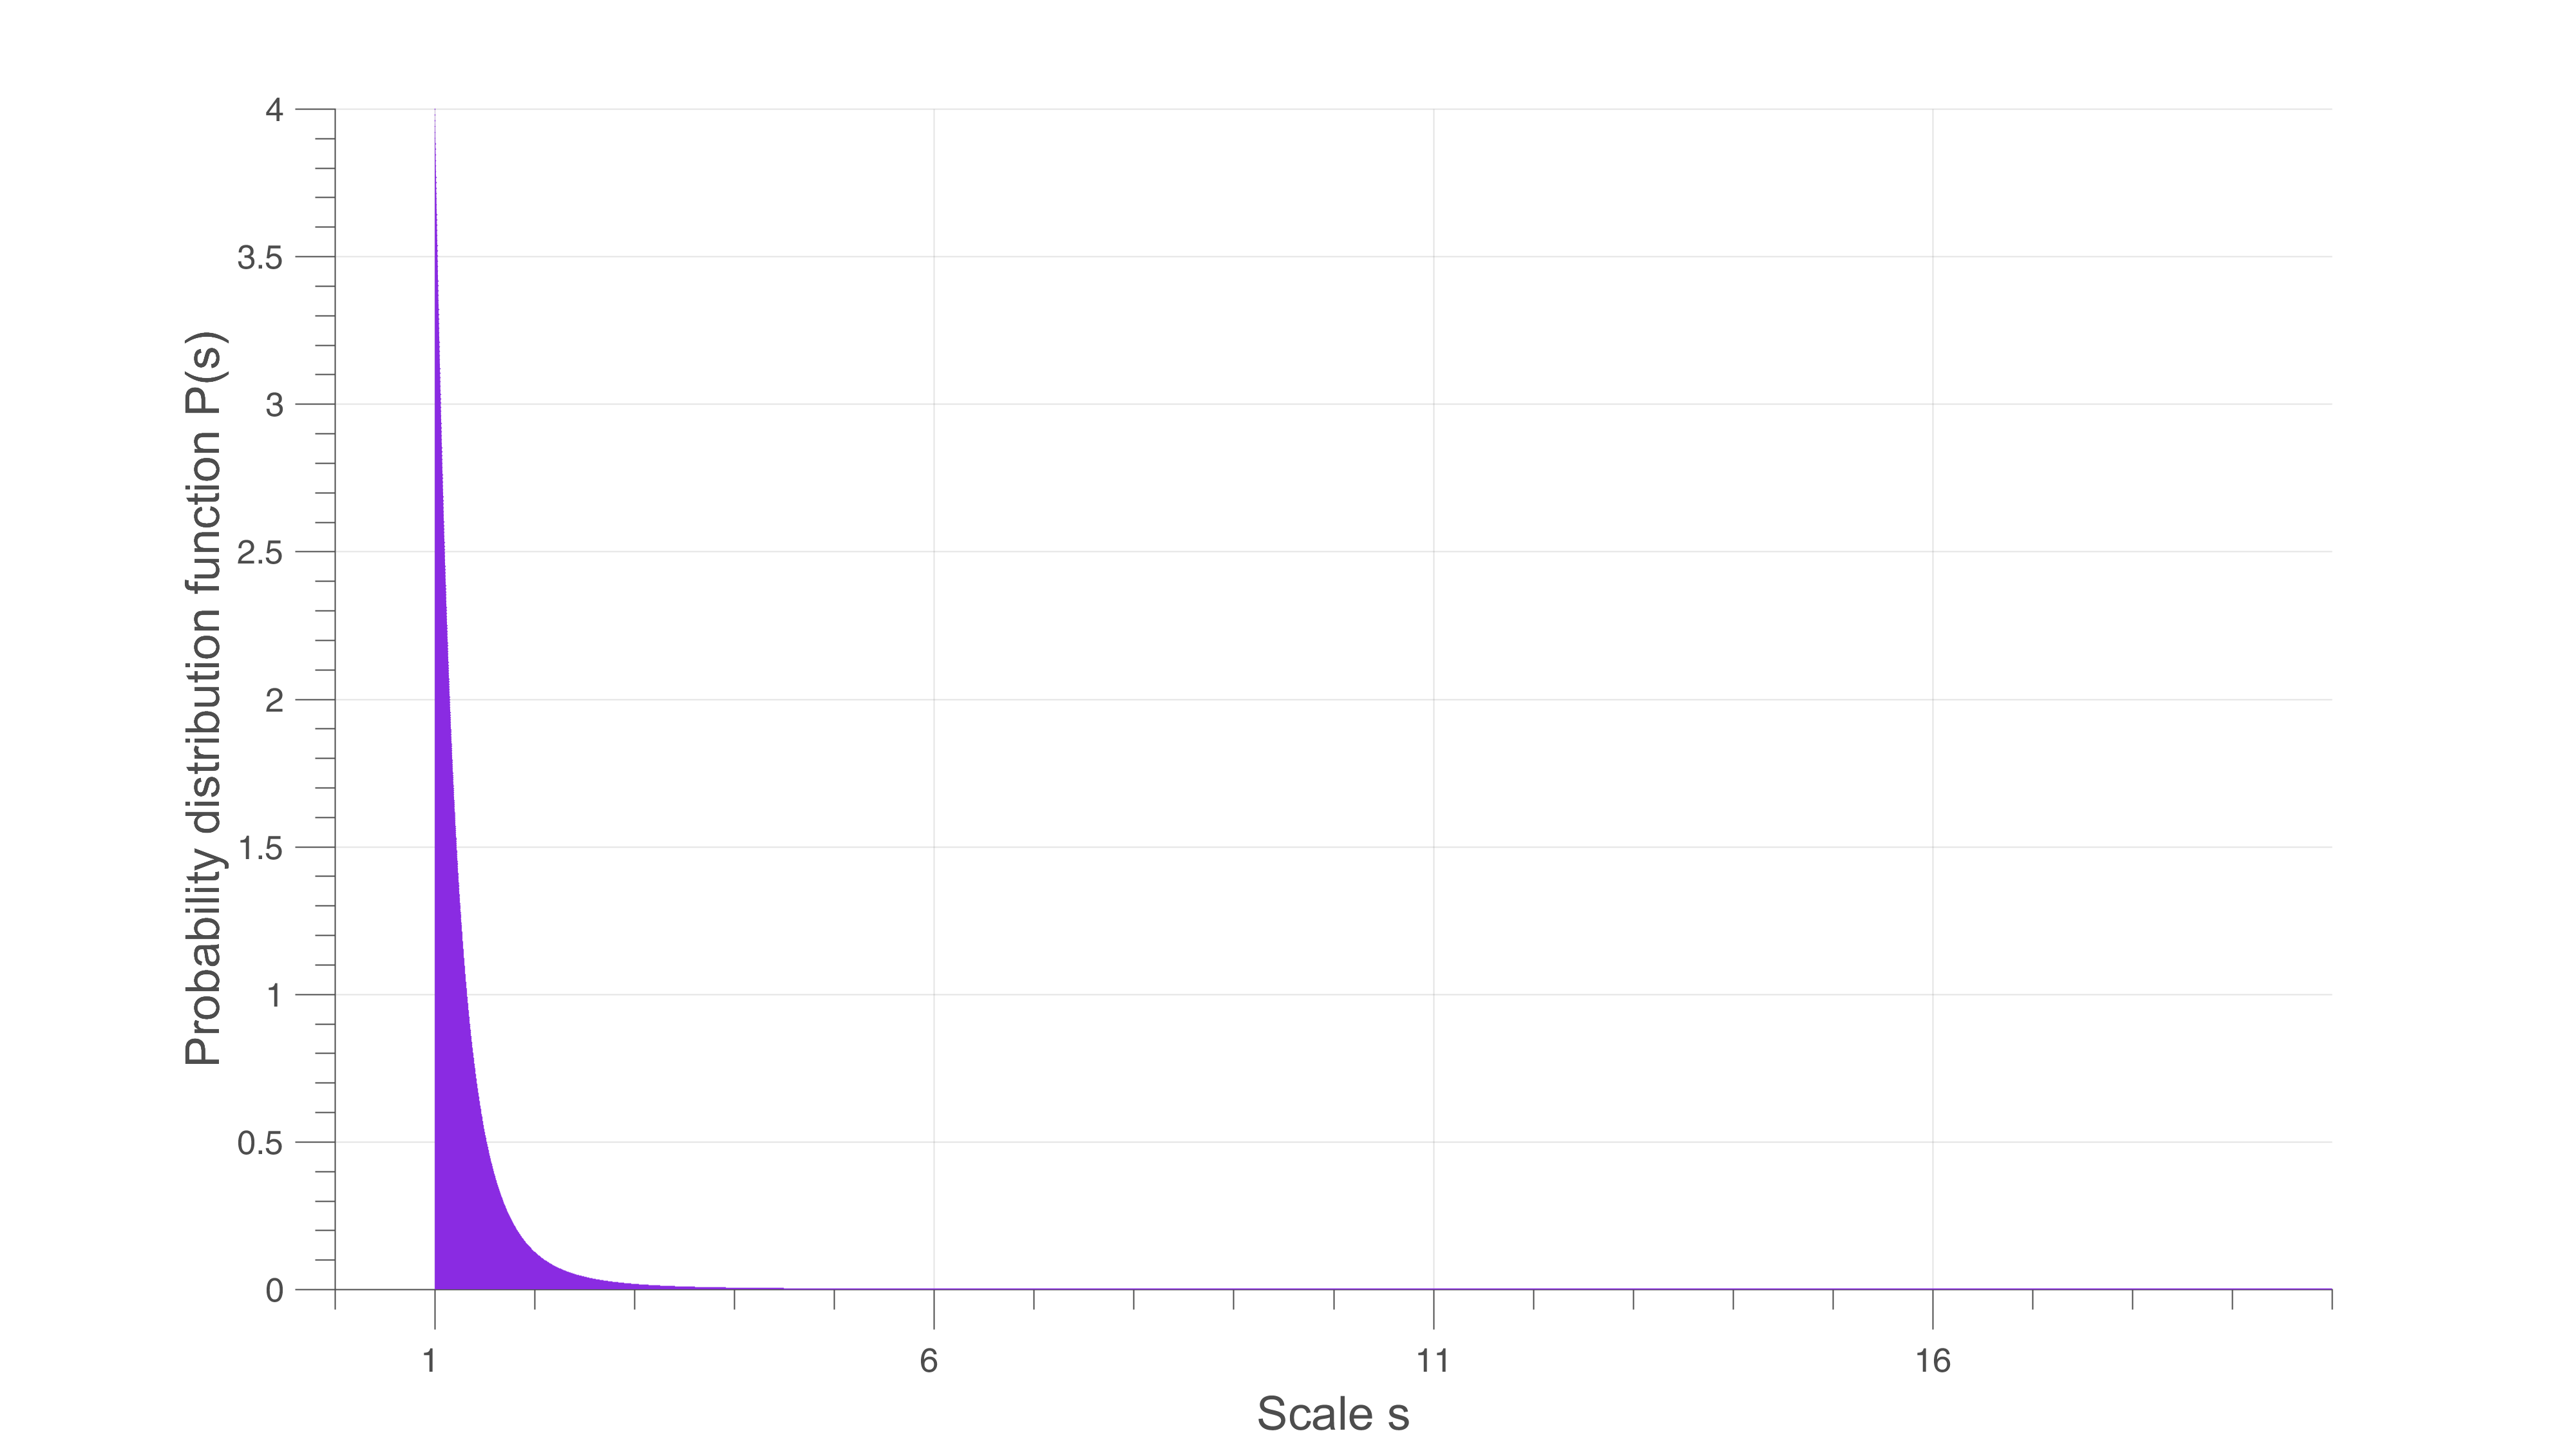
\includegraphics[width=0.9\textwidth]{figures//ps2.png} 
	\caption{Weakening scales $s$ probability distribution curve when $\beta=5$ }
	\label{ps2}
\end{figure}

\subsection{Yield function with mean stress effect}

Positive mean stress clearly reduces the fatigue life of the material. In design evaluation of multiaxial fatigue with mean stress, a simplified, conservative relation between mean stress and equivalent alternating stress is necessary. We can improve the model by modifying the yield function $\sigma_y$ and the localization tensor.

The idea is to consider as in Maitournam and Krebs\cite{Maitournam2011232} that the yield limit $\sigma_y$ can be reduced in presence of positive mean stress. The mesoscopic yield function can therefore be written as:
\begin{equation}
f\left(s\right)=||\uline{\uline{S}}(s)-\uline{\uline{b}}(s)||+\left( \lambda \Sigma_H-\sigma_y\right) /s\leqslant 0
\label{yieldfun}
\end{equation}
with $\uline{\uline{S}}$ denoting the deviatoric part of the stress tensor at microscale, and $\uline{\uline{b}}(s)$ the corresponding backstress at the same scale. The material remain in elastic regime when $f<0$ and in plastic regime when $f=0$.

\subsection{Local plastic model}
First we should describe the mesoscopic stress state.  The model considers a plastic 
behavior at the mesoscopic scale. The mesoscopic stress evolution equations are thus:

% \begin{numcases}{}
% 	\dot{\uline{\uline{S}}}(s,M,t)=dev\dot{\uline{\uline{\Sigma}}}(M,t)-\dfrac{E}{1+\nu}\dot{\uline{\uline{\varepsilon}}}^p(s,M,t), & Taylor-Lin scale transition model with unit localization tensor\cite{Bosia201239}.\\
% 	\dot{\uline{\uline{b}}}(s,M,t)=\dfrac{kE}{E-k} \dot{\uline{\uline{\varepsilon}}}^p(s,M,t) , & kinematic hardening model.\\
% 	\dot{\uline{\uline{\varepsilon}}}^p(s,M,t)=\gamma\dfrac{\partial f(s,M,t)}{\partial \uline{\uline{S}}}, & plastic flow rule assuming $\gamma=0$ when $f<0$ and  $\gamma\geqslant0$ when $f=0$.
% \end{numcases}
 
	\begin{equation}
    \dot{\uline{\uline{S}}}(s,M,t)=dev\dot{\uline{\uline{\Sigma}}}(M,t)-\dfrac{E}{1+\nu}\dot{\uline{\uline{\varepsilon}}}^p(s,M,t), 
	\end{equation}
     which defines a Taylor-Lin scale transition model with unit localization tensor\cite{Bosia201239}.
		\begin{equation}
		\dot{\uline{\uline{b}}}(s,M,t)=\dfrac{kE}{E-k} \dot{\uline{\uline{\varepsilon}}}^p(s,M,t), 
		\end{equation}
		which is our kinematic hardening model.
		\begin{equation}
		\dot{\uline{\uline{\varepsilon}}}^p(s,M,t)=C\dfrac{\partial f(s,M,t)}{\partial \uline{\uline{S}}}, 
		\end{equation}
		which is the associated plastic flow rule assuming $C=0$ when $f<0$ and  $\gamma\geqslant0$ when $f=0$.

Here E denotes the Young's modulus and k the hardening parameter. The local dissipated energy rate per volume at weakening scales $s$  is given by the local entropy dissipation:
\begin{equation}
	\dot{w}(s,M,t)=(\uuline{S}-\uuline{b})(s,M,t):\uuline{\dot{\varepsilon}}^p(s,M,t).
	\label{dissipated}
\end{equation}

\section{Construction of an energy based fatigue approach}

In a preliminary step, we will consider a simple macroscopic loading history $\uuline{\Sigma}(M, t)$ which is uniaxial
and time periodic of deviatoric amplitude $S_{max}$, and a Von Mises flow rule to see if we get a prediction of local failure for a number of cycles $N_F$ varying as $\Sigma^{-\beta}.$


\noindent
In uniaxial cyclic loading, there will be 3 kinds of loading patterns, as is shown in \figref{backstress}:

\vspace{6pt}
\begin{enumerate}
	
	\item	Elastic regime, in phase 2 and 4,where $\dot{\uline{\uline{\varepsilon}}}^p(s,M,t)=0$ ,  and $|\uline{\uline{S}}-\uline{\uline{b}}|< \left( \sigma_y-\lambda \Sigma_H\right)/s. $ 
	\vspace{6pt}
	
	\item Plastic regime according to plastic flow rule, with increasing plastic deformation, in phase 5 and 1, where	$\dot{\uline{\uline{\varepsilon}}}^p(s,M,t)=C\dfrac{\uline{\uline{S}}(s)-\uline{\uline{b}}(s)}{||\uline{\uline{S}}(s)-\uline{\uline{b}}(s)||}> 0$ with  $C= dev\dot{\uline{\uline{\Sigma}}}\left(\dfrac{kE}{E-k}+\dfrac{E}{1+\nu} \right) ^{-1}$ ,  with $\uline{\uline{S}}-\uline{\uline{b}}= \left(\sigma_y-\lambda \Sigma_H\right)/s$ and $\dot{\uline{\uline{S}}}-\dot{\uline{\uline{b}}}=0.$ 
	\vspace{6pt}
	
	\item Plastic regime in the other direction, in phase 3, there is	$\dot{\uline{\uline{\varepsilon}}}^p(s,M,t)<0$,  then $\uline{\uline{S}}-\uline{\uline{b}}=- \left(\sigma_y-\lambda \Sigma_H\right)/s$ and $\dot{\uline{\uline{S}}}-\dot{\uline{\uline{b}}}=0$ 
	
\end{enumerate}	

\begin{figure}[!h]
	\centering
	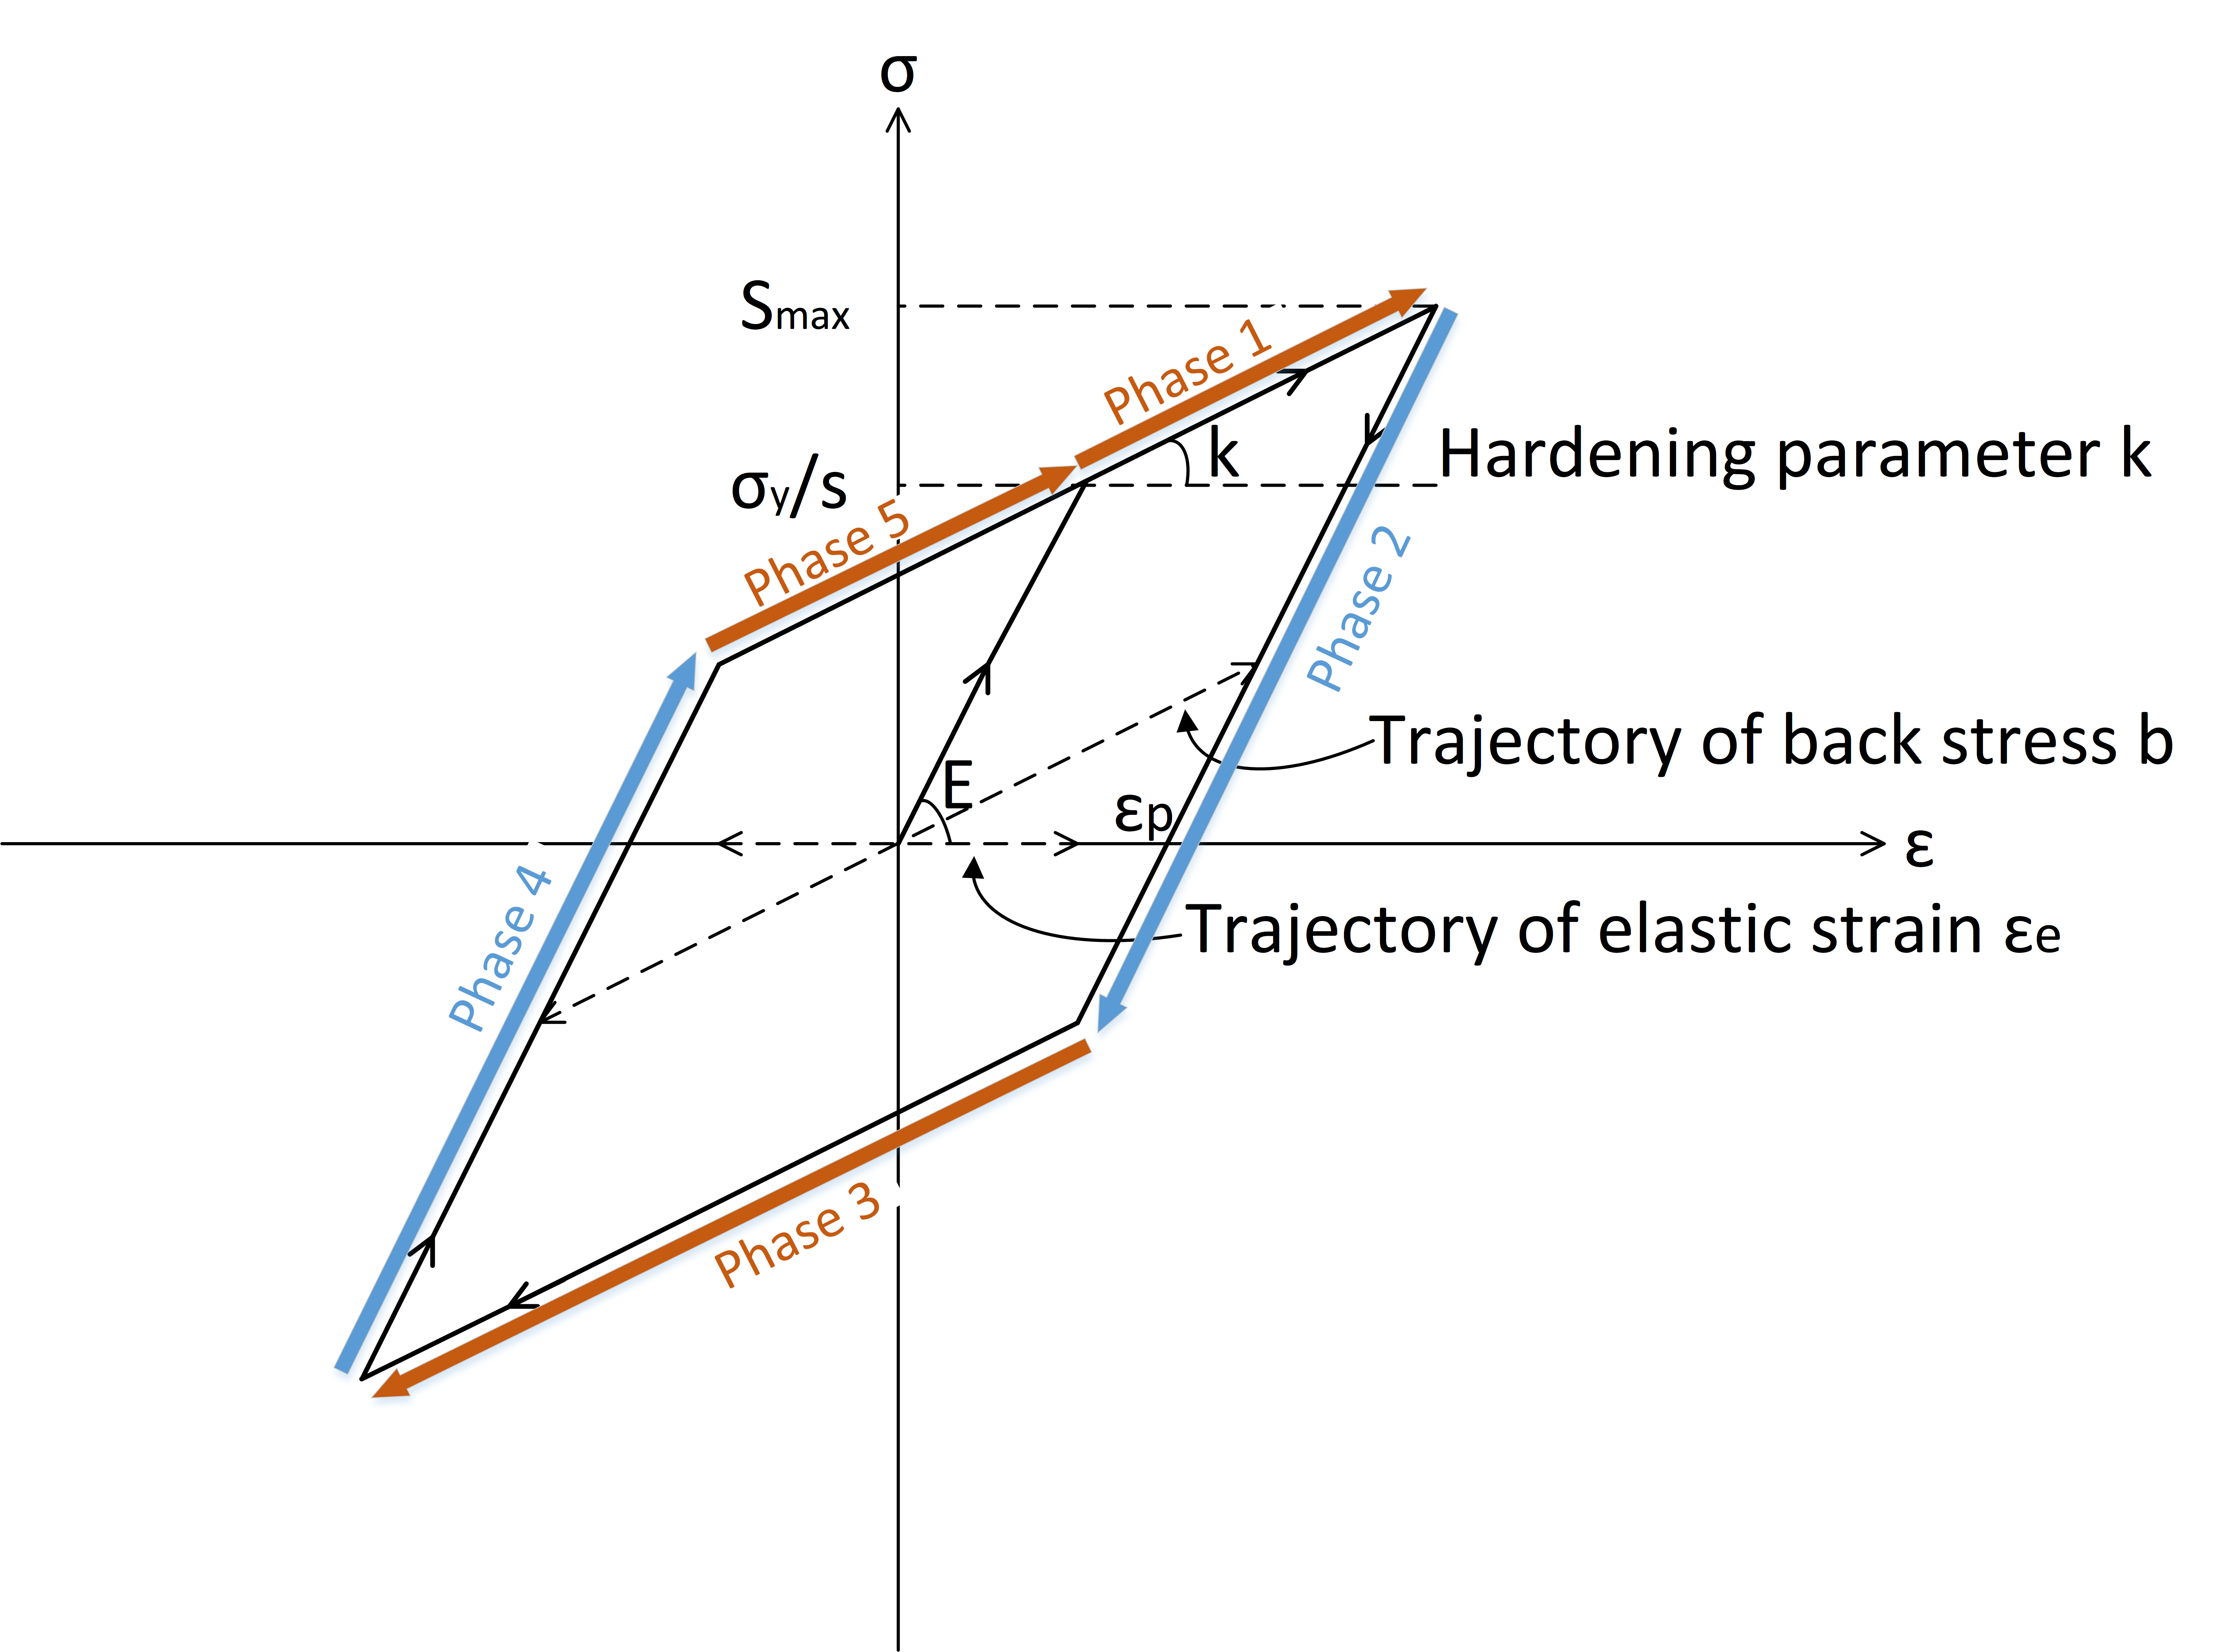
\includegraphics[width=0.9\textwidth]{figures//backstress.png} 
	\caption{Uniaxial load with plastic dissipation}
	\label{backstress}
\end{figure}

In phase 1, a direct analysis yields the energy dissipation at scale $s$:
\begin{equation}dW=(S-b)d\varepsilon^p=\dfrac{(E-k)(1+\nu) }{E(E+k\nu)}\dfrac{ \left(\sigma_y-\lambda \Sigma_H\right)}{s}\left(S_{max}-\dfrac{ \left(\sigma_y-\lambda \Sigma_H\right)}{s}\right)
\label{dw}
\end{equation}

A similar analysis yields $$dW(phase 1)=dW(phase 5)=\dfrac{1}{2}dW(phase 3).$$

We can then calculate  the local dissipated energy $W$  at point $M$ during one cycle by cumulating the input of all sub-scales which result in plastic regime with their probabilities \cite{zepeng}.
\begin{equation}
\begin{split}
W_{cyc}&=4\int_{ \left(\sigma_y-\lambda \Sigma_H\right) /S_{max}}^{\infty}dW(s,M,t)P(s)ds
\\&=4\int_{ \left(\sigma_y-\lambda \Sigma_H\right) /S_{max}}^{\infty}\dfrac{(E-k)(1+\nu) }{E(E+k\nu)}\dfrac{ \left(\sigma_y-\lambda \Sigma_H\right)}{s}\left(S_{max}-\dfrac{ \left(\sigma_y-\lambda \Sigma_H\right)}{s}\right)\left( \beta-1\right) s^{-\beta}ds
\\&=\dfrac{4(E-k)(1+\nu)\left( \beta-1\right) }{ E(E+k\nu)\beta\left( \beta+1\right) }\dfrac{S_{max}^{\beta+1}}{ \left(\sigma_y-\lambda \Sigma_H\right)^{\beta-1}}.
\end{split}
\label{eq:w}
\end{equation}

So we have a power law relationship between stress intensity and the dissipated energy per cycle as Eq.\eqref{eq.wcyc}.
\begin{equation}
W_{cyc}=C_1S_{max}^{\beta+1},
\label{eq.wcyc}
\end{equation}
with 
$$C_1=f(\lambda,\beta)=\dfrac{4(E-k)(1+\nu)\left( \beta-1\right) }{ E(E+k\nu)\beta\left( \beta+1\right)\left(\sigma_y-\lambda \Sigma_H\right)^{\beta-1} }.$$
 If the dissipated energy accumulates linearly until a failure value $W_0$, we can get directly the number of cycles to failure from Eq.\eqref{eq.NFcyc}:
\begin{equation}
N_{F}=\dfrac{W_0}{W_{cyc}}=\dfrac{W_0}{C_1}S_{max}^{-\beta-1}.
\label{eq.NFcyc}
\end{equation}
As for the time to failure in cyclic loading, there is:
$$T_{F}=N_{F}t_{cyc}.$$
From Eq.\eqref{eq:w}, we then obtain that the model predicts as expected a power law dependence in function of $S_{max}$.
However, experiments shows that the damage or the energy accumulation of a material evolves non-linearly in time. We should introduce below a method to handle such a nonlinearity.

\section{Nonlinearity of damage accumulation}
\subsection{Energy approach with Chaboche law}
The Chaboche law\cite{lemaitre1990mechanics} is essentially a damage incremental law for cyclic loading of stress intensity $\sigma$ with a deviatoric part ${A}_{\uppercase\expandafter{\romannumeral2}}$ and hydrostatic part $\Sigma_H$, defining the damage increase by:

 \begin{equation}\delta D = \left( 1 -(1-D)^{\gamma+1}\right)^\alpha \left(\frac{{A}_{\uppercase\expandafter{\romannumeral2}} }{M(\sigma_H)\left( 1-D\right)}\right)^\gamma \delta N
 \label{chabochemulti}
 \end{equation} 
 
With ${A}_{\uppercase\expandafter{\romannumeral2}}^*={A}_{\uppercase\expandafter{\romannumeral2}}/\left( 1-D\right) $ evolving with damage $D$. And the mean stress effect is in both exponential $\alpha$ and denominator $M(\sigma_H)$.
$$\alpha=1 - a\left\langle \dfrac{\dfrac{1}{2}\sigma_{vm}(t)-\sigma_{-1}M(\sigma_H) }{\sigma_{u} -\sigma_{vm}(t)}\right\rangle,$$
$$M(\sigma_H) =M_0 \left(1-3c\sigma_{H,max}(t) \right).$$
 
Eq.\eqref{chabochemulti} writes equivalently as Eq.\eqref{integration}:
   \begin{equation}\delta [1-(1-D)^{\gamma+1}]^{1-\alpha}=(1-\alpha)(\gamma+1)\left(\dfrac{{A}_{\uppercase\expandafter{\romannumeral2}} }{M(\Sigma_H)}\right)^\gamma \delta N=\dfrac{1}{N_F(\sigma)}\delta N.
   \label{integration}
   \end{equation}
Here $N_F(\sigma)$ denotes the number of cycles at intensity $\sigma$ to failure as obtained by integration of Eq.\eqref{integration} from $D=0$ to $D=1$. In our model, in case of a simple uniaxial cyclic loading, we propose to replace $\dfrac{1}{N_F(\Sigma)}$ which is the relative unit increment of energy by $\dfrac{W_{cyc}(\Sigma)}{W_0}$.



The nonlinear damage incremental law using energy dissipation:
\begin{equation}
\begin{split}
  \delta D &=\dfrac{\left( 1 -(1-D)^{\gamma+1}\right)^\alpha}{\left(1-D \right)^\gamma} \delta W
  \\&= \dfrac{\left( 1 -(1-D)^{\gamma+1}\right)^\alpha}{\left(1-D \right)^\gamma} \dfrac{W_{cyc}\delta N}{W_0}
  \\&= \dfrac{\left( 1 -(1-D)^{\gamma+1}\right)^\alpha}{\left(1-D \right)^\gamma} \dfrac{4(E-k)(1+\nu)\left( \beta-1\right) }{ E(E+k\nu)\beta\left( \beta+1\right) }\dfrac{S_{max}^{\beta+1}}{\left(\sigma_y-\lambda \Sigma_H\right)^{\beta-1}}\dfrac{\delta N}{W_0}.
\end{split}
\label{recoverchaboche}
\end{equation} 

We compare Eq.\eqref{chabochemulti} and Eq.\eqref{recoverchaboche}, in Chaboche model there is:
$$\beta+1=\gamma. $$

Similar to Eq.\eqref{integration}, we define here the ''equivalent damage'' $\hat{D}$ in Eq.\eqref{eq.Dhat}:

\begin{equation}
\hat{D}=1-(1-D)^{\gamma+1},
\label{eq.Dhat}
\end{equation}
with $D$ the damage variable introduced by Chaboche in its model to scale the stress intensity:
$${A}_{\uppercase\expandafter{\romannumeral2}} \longrightarrow \dfrac{{A}_{\uppercase\expandafter{\romannumeral2}}}{1-D}.$$

We have 

$\bullet$ $\hat{D}=0$ when $D=0$(undamaged material),

$\bullet$ $\hat{D}=1$ when $D=1$(failure of material),	

and a nonlinear relation in between as in \figref{fig.Dhat}:
$$\delta\hat{D}=\left(\gamma+1 \right)\left( 1-D\right)^\gamma \delta D$$	
\begin{figure}
	\centering
	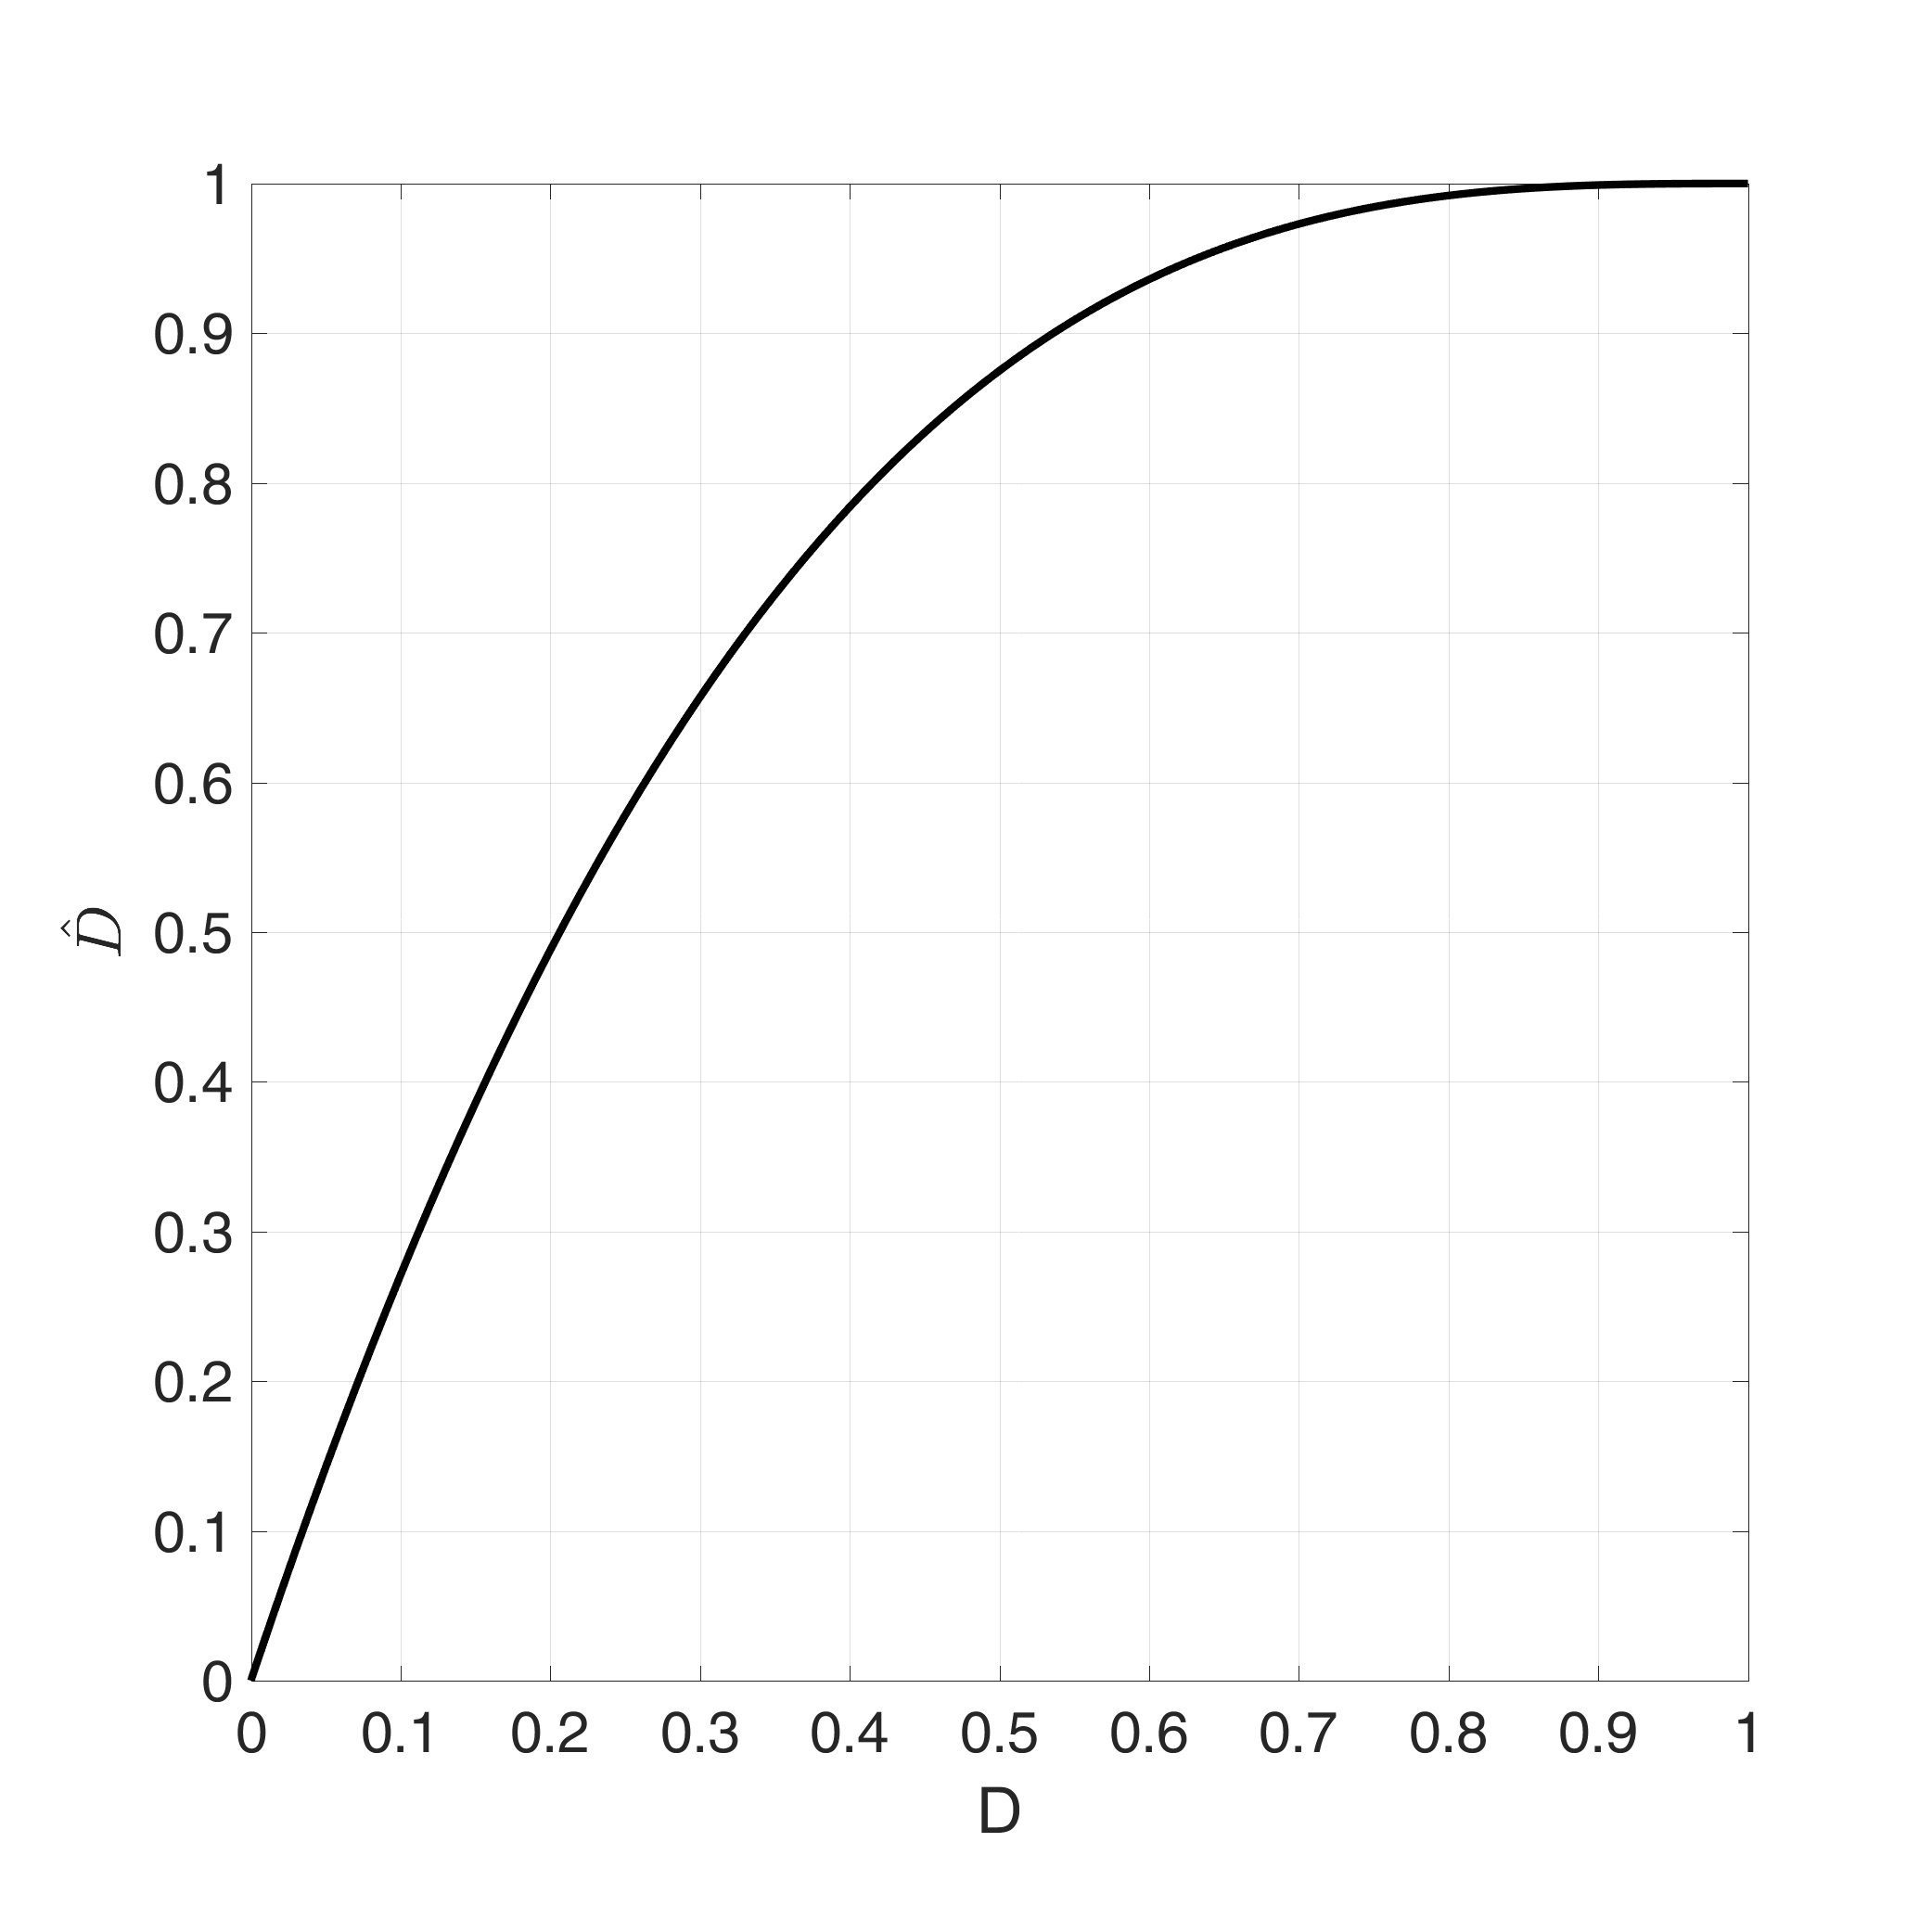
\includegraphics[width=0.5\textwidth]{figures//Dhat.png} 
	\caption{The relation between $\hat{D}$ and $D$ when $\gamma=2$}
	\label{fig.Dhat}
\end{figure}

Now in our model we use the same growth rule as in Chaboche in cyclic load regime:
\begin{equation}
\delta D=D^\alpha\dfrac{\delta W}{W_0}=D^\alpha\dfrac{W_{cyc}\delta N}{W_0}.
\label{eq.DWcyc}
\end{equation}

The number of cycles to failure in constant loading case, obtained by integrating $D$ from 0 to 1 is:
\begin{equation}
N_F=\dfrac{W_0}{\left( 1-\alpha\right)W_{cyc} }=\dfrac{W_0}{\left( 1-\alpha\right)C_1}S_{max}^{-\beta-1}.
\label{eq.NFWcyc}
\end{equation}
 
From Eq.\eqref{eq.NFWcyc}, we see $(-\beta-1)$ is related to the slop in S-N curve and $\frac{W_0}{C_1}$ defines the number of cycles to failure.
 
 
\subsection{Generalized damage accumulation}
Formula \eqref{integration} is a general accumulation law which can be applied for any cyclic loading sequence provided that we can identify the multiscale value of the dissipated energy per cycle. 

But the notion of cycle itself may be hard to identify for general loadings. The idea is then to replace the relative increment of dissipated energy per cycle by the relative increment of dissipated energy per unit time, yielding in Eq.\eqref{eq.DW}:
\begin{equation}
\delta D= D^\alpha \dfrac{W}{W_0} = D^\alpha \dfrac{\dot{W}\delta t}{W_0}
\label{eq.DW}
\end{equation}

The time to failure, obtained by integrating $D$ from 0 to 1 is:
\begin{equation}
T_F=\dfrac{W_0}{\left( 1-\alpha\right) \dot{W}}.
\label{eq.tf}
\end{equation}

In differential form, the relation \eqref{eq.diffform} writes from Eq.\eqref{eq.DW} and Eq.\eqref{eq.tf}:
\begin{equation}
\delta D^{1-\alpha}=\frac{\delta t}{T_F}.
\label{eq.diffform}
\end{equation}

When we integrate Eq.\eqref{eq.DW} from $0$ to $D$ at constant loading conditions. The damage, expressed as a function of $t/T_F$ is:
\begin{equation}
D=\left( \frac{t}{T_F}\right) ^{\frac{1}{1-\alpha}}.
\label{eqD}
\end{equation}
This expression is in good agreement with experimental results\cite{lemaitre1990mechanics}. 

In a general loading case, $\dot{W}$ is the microscopic energy dissipation rate of unit defect and $W_0$ is the energy threshold of unit defect. By integrating Eq.\eqref{dissipated} over all microscales, we get:
\begin{equation}\dot{W}(M,t)=\int_{s=1}^{\infty}\dot{w}(s,M,t)P(s)ds=\int_{s=1}^{\infty}\left(\uuline{S}-\uuline{b} \right) (s,M,t):\uuline{\dot{\varepsilon}^p}(s,M,t)P(s)ds.\label{Wdot}
\end{equation}
The evolution of $\uuline{S}$, $\uuline{b}$ and $\uuline{\dot{\varepsilon}}^p$ are given previously. Eq.\eqref{eq.DW} and \eqref{Wdot} are therefore our proposed damage incremental law with energy dissipation.

This is a nonlinear law with a constant $\alpha$, there will be no sequence effect. In other words,
when applying two successive cycles of different intensities, the failure will occur at the same number of cycles whatever the order of the loading(high then low versus low then high). In numerical implementation of complex loading case, to take into account the load sequence effect, $\alpha$ changes at every time step.

We introduce $s_{min}$, which is the minimum scale that causes energy loss:
$$s_{min}=\dfrac{\left(\sigma_y-\lambda \Sigma_H\right)}{S_{max}}.$$
To take into account the sequence effect, the parameter $\alpha$ should change with $S_{max}$ in order to handle change of cycle intensity and the influence on fatigue life.

\subsection{Sequence effect}

Many fatigue damage accumulation models are based on the two level loading experiments which is one of the basic random loading analysis. To facilitate our verification of the law we use two-stress level loading, the specimen is firstly loaded at stress $\Sigma_1$ for $T_1$ cycles and then at stress $\Sigma_2$ for $T_2$ cycles until failure. We can then observe if the experimental results are satisfactory.

In Chaboche model, the proposition of $\alpha$ is:

\begin{equation}
\alpha = 1 - a\left\langle \frac{ \sigma_{eq}-\sigma_{fatigue}}{ \sigma_{u} - \sigma_{eq}}\right\rangle.
\end{equation}

Our proposal of $\alpha$ is expressed as Eq.\eqref{eq.alpha}:
\begin{equation}
\alpha=1-a\left\langle \dfrac{\frac{1}{s_{min}}}{1-\frac{1}{s_{min}}} \right\rangle^\beta .
\label{eq.alpha}
\end{equation}

There is no notion of fatigue limit in our model, $\sigma_{faigue}=0$. The intensity of loading
 $$\frac{ \sigma_{eq}-\sigma_{fatigue}}{ \sigma_{u} - \sigma_{eq}}= \frac{ 1}{\frac{\sigma_{u}}{\sigma_{eq}} -1}$$
 is measured by 
$$\left( \dfrac{\frac{1}{s_{min}}}{1-\frac{1}{s_{min}}}\right) ^\beta=\left(\dfrac{1}{s_{min}-1} \right) ^\beta.$$
This means that we measure the distance of load to ultimate failure by local variable $s_{min}$ through 

$$\frac{\sigma_{u}}{\sigma_{eq}} -1 \longrightarrow \left( s_{min}-1\right) ^\beta $$

We use the power law related to energy dissipation parameter $\beta$ to magnify large stress impact and minify lower stress damage. Here the power $\beta$ and has anti-correlation with $T_F$ in low cycle fatigue regime but has positive correlation in high cycle fatigue regime. 

After loading time $T_1$, we have from Eq.\eqref{eqD}, a damage $D_1$ given by:
\begin{equation}
\left( 1-D_1\right) ^{1-\alpha_1}=\dfrac{T_1}{T_{F1}}
\label{23a}
\end{equation}
By integrating Eq.\eqref{diffform} from $D=D_1$ to $D=1$, we get:
\begin{equation}
1-\left( 1-D_1\right)^{1-\alpha_2}=\dfrac{T_2}{T_{F2}}
\label{23b}
\end{equation}

From Eq.\eqref{23a} and Eq.\eqref{23b}, after elimination of $\left( 1-D_1\right)$ we get:
\begin{equation} 
\dfrac{T_2}{T_{F2}} =1-\left( \dfrac{T_1}{T_{F1}}\right) ^\eta,
\end{equation}
with
\begin{equation}
\eta=\dfrac{1-\alpha_2}{1-\alpha_1}.
\label{eq.eta}
\end{equation}

In the case of high-low loading sequence there is $\Sigma_1>\Sigma_2$, meaning $S_{max1}>S_{max2}$, which gives $\alpha_1<\alpha_2$:
$$\eta=\frac{1-\alpha_2}{1-\alpha_1}<1;\,
 \frac{T_2}{T_{F2}}=1-\left( \frac{T_1}{T_{F1}}\right) ^\eta<1-\frac{T_1}{T_{F1}};\,
\frac{T_1}{T_{F1}}+\frac{T_2}{T_{F2}}<1.$$

The cumulative damage under high-low loading sequence, as we deduced, has the addition of partial lives less than unit. Similarly, the cumulative damage under low-high loading sequence has addition of partial lives more than 1.
$$\frac{T_1}{T_{F1}}+\frac{T_2}{T_{F2}}>1$$
 The curve is depicted in \figref{fig.sequence}.
\begin{figure}[!h]
	\centering
	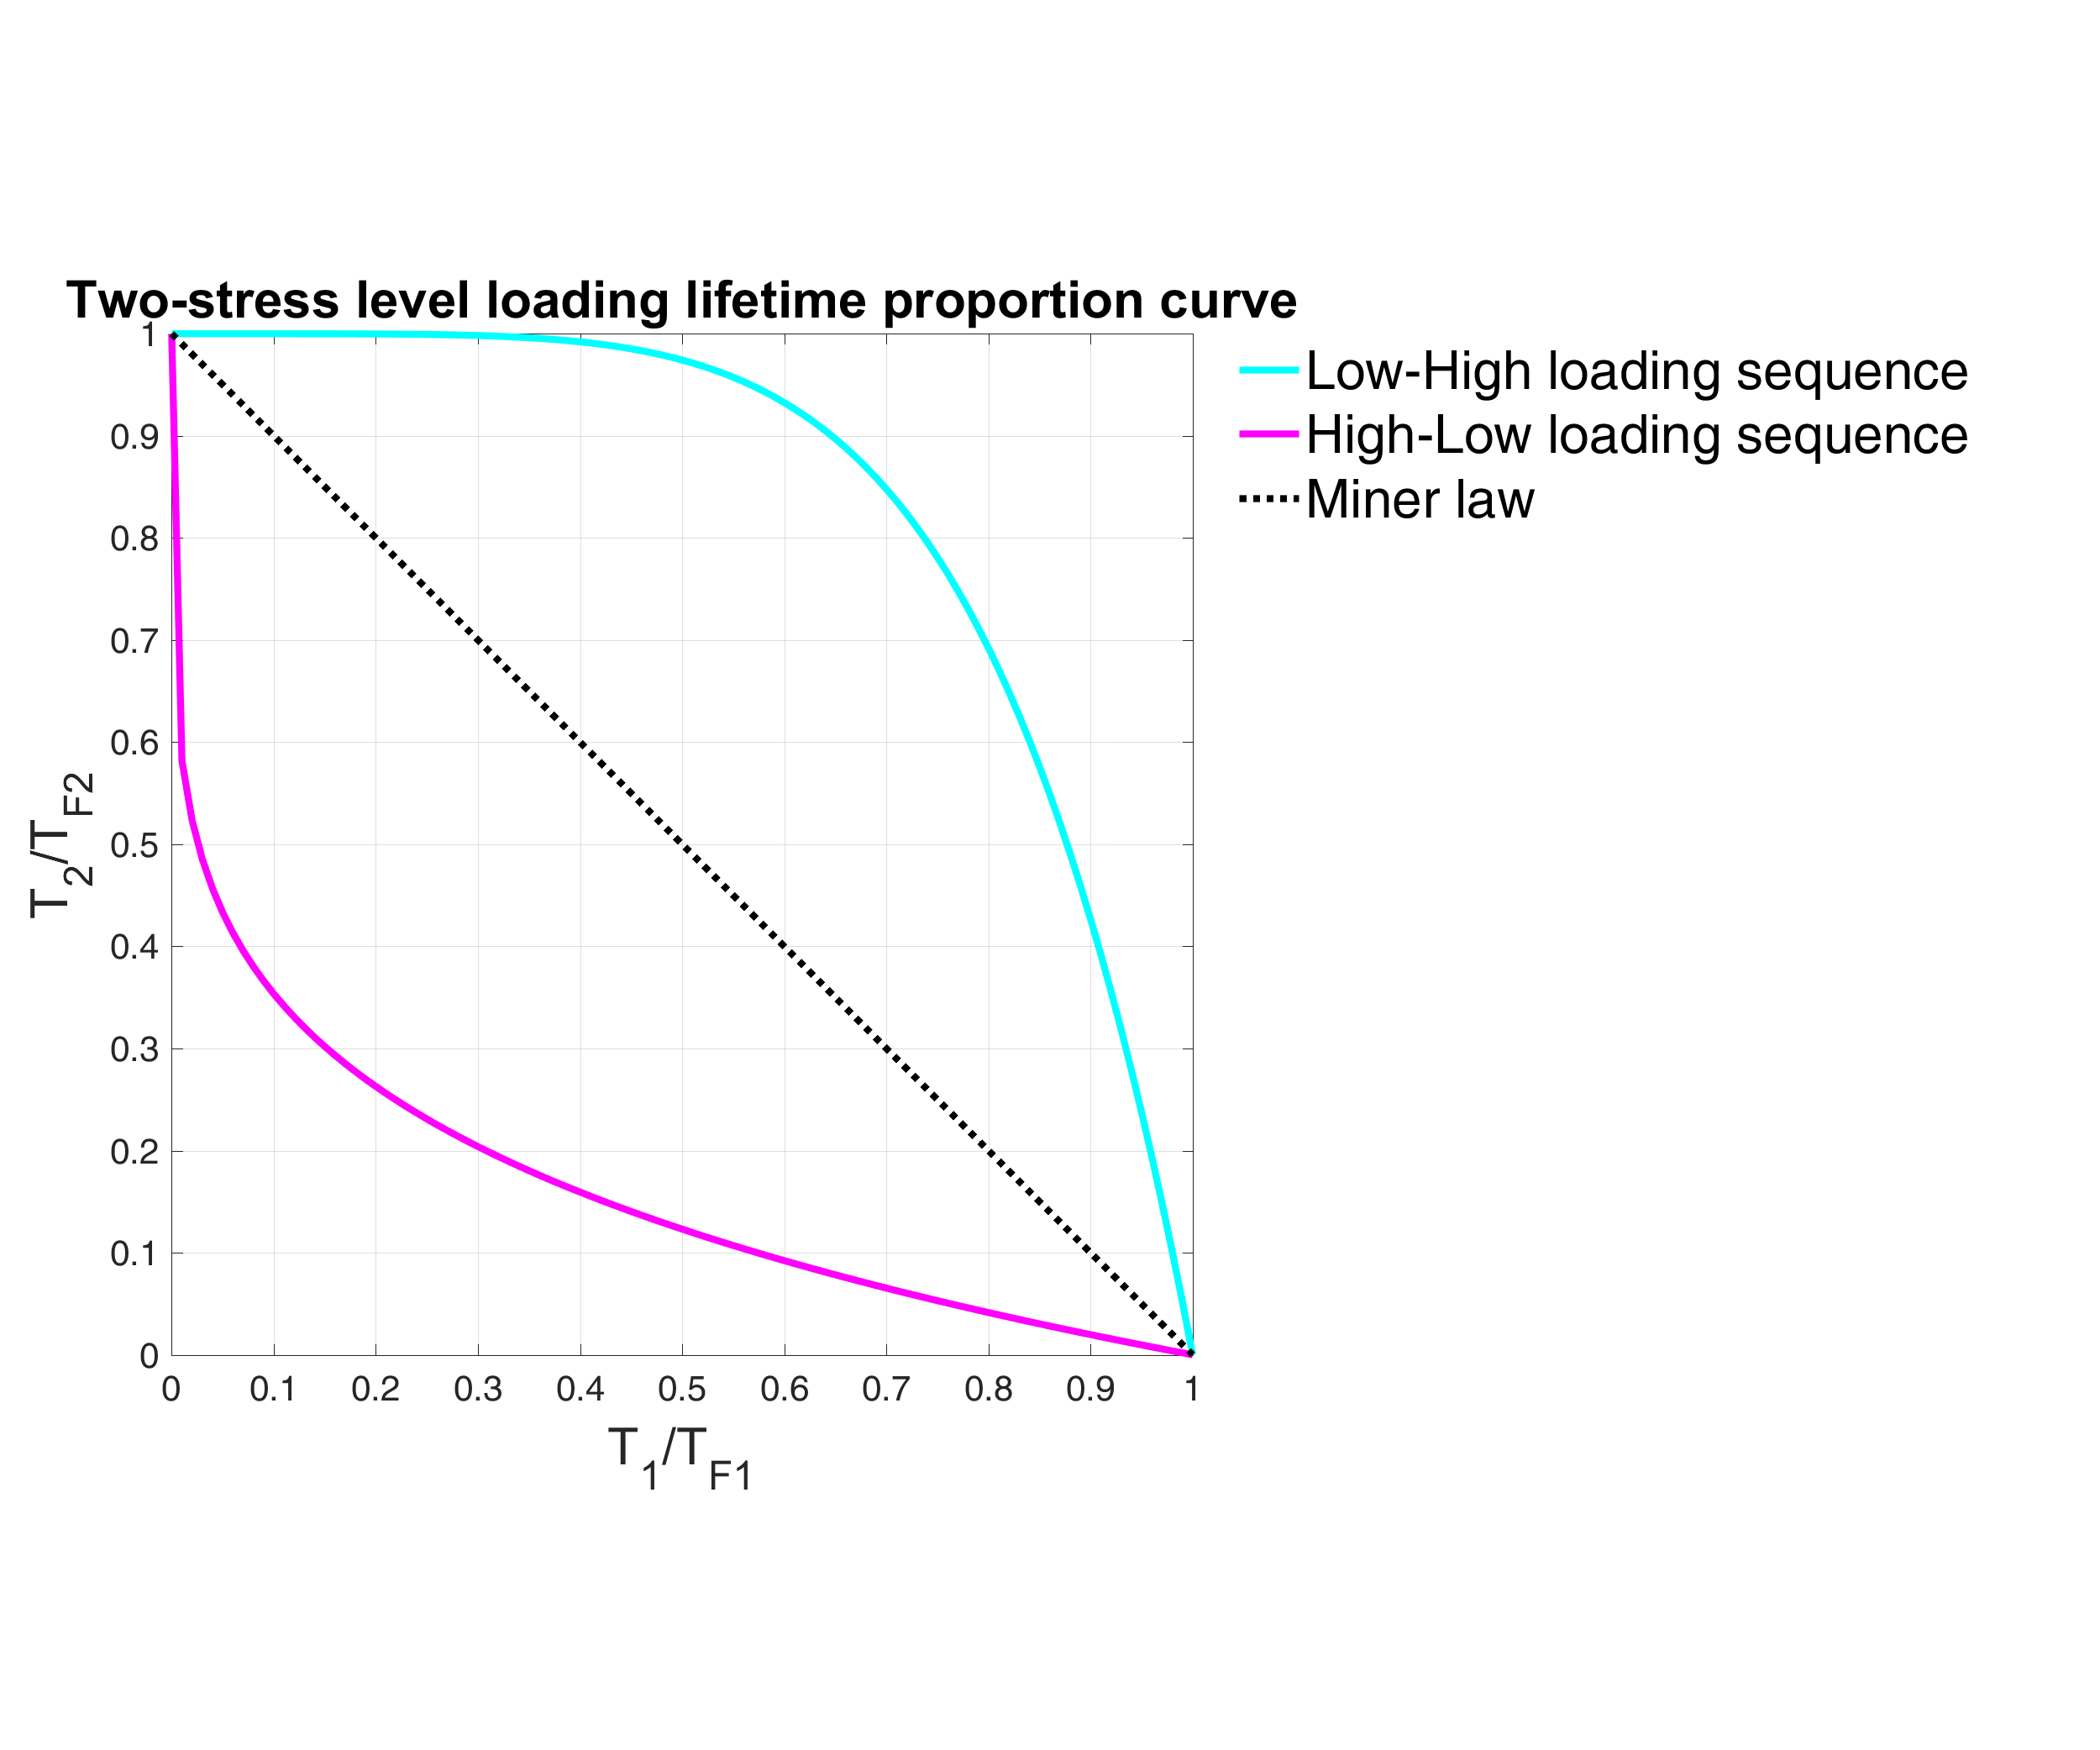
\includegraphics[width=\textwidth]{figures//sequence.png} 
	\caption{High to low and low to high loading sequence comparison}
	\label{fig.sequence}
\end{figure}
For constant two-level stress loading, $\alpha_1=\alpha_2$, the Chaboche law returns to the Miner rule where:
$$\frac{T_1}{T_{F1}}+\frac{T_2}{T_{F2}}=1$$

\section{Numerical strategy}
\subsection{Integration rules for $\dot{W}$ and $\delta D$}
Our first approach takes one cycle as unit time. We compute analytically the energy dissipation at each scale during this cycle. The method is valid for simple loading history and which includes the integration on all weakening scales. The damage $D$ is accumulated after each cycle.

However, there are certain limitations of this method. Firstly we need a load history decomposition in cycles. Secondly in real life the perfect close loop cycle is hardly applicable.

Thus we propose in Eq.\eqref{eq.DW} a more general method which can be integrated by a step by step strategy. We compute numerically the dissipation at different scales using an implicit Euler time integration of the constitutive laws of section 1.4. After which we make a numerical integration on different scales. Then we can update the damage and go to next time step. 

Instead of doing the scale integration directly which can be difficult for complex loading, the Gaussian Quadrature rule with Legendre points is used to give the value of local dissipated energy rate.

To use the Gaussian quadrature rule the limit range of integral must be from $-1$ to $1$, while the total dissipated energy  is expressed by integrating all the weakening scale $s$ ranging from 1 to infinity with their occurrence probabilities:
$$\dot{W}=\int_{1}^{\infty}\dot{w}(s) (\beta-1)(s)^{-\beta}ds.$$

\noindent
To change the limit range of integral from $[1,\infty]$ to $[1,0]$ we take as new integration variable
$u(s)= s^{-p}$ with $p=\beta-1$, yielding $u(1)=1$ and  $u(\infty)=0$ with
$$du=-ps^{-p-1}ds$$ 
that is
$$du=(-\beta+1) s^{-\beta}ds=(-\beta+1)s^{-\beta} ds.$$
Therefore the dissipated energy summed on all scales is:
\begin{equation}
\begin{split}
\dot{W}&=\int_{1}^{\infty}\dot{w}(s) (\beta-1)(s)^{-\beta}ds
\\&=\int_{1}^{0}\dot{w}\left( u^{\frac{1}{1-\beta}}\right) (\beta-1) \frac{1}{-\beta+1}du
\\&=\int_{0}^{1}\dot{w}\left( u^{\frac{1}{1-\beta}}\right) (\beta-1) \frac{1}{\beta-1}du
\\&=\int_{0}^{1}\dot{w}\left( u^{\frac{1}{1-\beta}}\right)du
\\&=\frac{1}{2}\int_{-1}^{1}\dot{w}\left[  \left( \frac{x+1}{2}\right) ^{\frac{1}{1-\beta}}\right] dx
\end{split}
\label{allscale}
\end{equation}
given $u=\dfrac{x+1}{2}$.

So the dissipated energy rate integrated over all scales takes the form of Eq.\eqref{allscalerate}:
\begin{equation}
\dot{W}=\frac{1}{2}\int_{-1}^{1}\dot{w}\left[  \left( \frac{x+1}{2}\right) ^{\frac{1}{1-\beta}},t\right] dx\approx\frac{1}{2}\sum_{i}\omega_i\dot{w}\left[  \left( \frac{x_i+1}{2}\right) ^{\frac{1}{1-\beta}},t\right],
\label{allscalerate}
\end{equation}
where $\omega_i$ and $x_i$ are respectively the weights and nodes of the Gauss Legendre integration rule used for the numerical integration. The use of Gaussian Quadrature rule changes the integrand s from infinity to finite fixed values without affecting the integration results. In this work, we used 64 points\cite{legendre}.

After changing the integration limit, $\left( \dfrac{x+1}{2}\right) ^{\frac{1}{1-\beta}}$ represents the weakening scale $s$. 

Damage accumulation is deduced from Eq.\eqref{eq.DW}:
\begin{equation}
D_{n+1}=D_n+D_n^\alpha\dfrac{W}{W_0}
\label{eq.damage}
\end{equation}

with $W=\dot{W}dt$
We upgrade the damage step by step following Eq.\eqref{eq.damage}. When $D$ reaches one, the material fails. 

\subsection{Regime determination under multiple scales}
The material could be both in elastic and plastic regime at different scales. To be more elaborate, we reuse the fundamental equations in different regimes. At scale $s$, we have a dissipation rate given by:
$$\dot{w}(s)=\left( \uline{\uline{S}}-\uline{\uline{b}}\right):\dot{\uline{\uline{\varepsilon}}}^p, $$
which differs between plastic and elastic regime.

\vspace{6pt}
\noindent
\textbf{Elastic regime:}

\vspace{6pt}
\noindent
There we have
plastic strain rate
$\dot{\uline{\uline{\varepsilon}}}^p=0$, back stress rate $\dot{\uline{\uline{b}}}=0$ and deviatoric stress rate $\dot{\uline{\uline{S}}}=dev\dot{\uline{\uline{\Sigma}}}$, leading to
$$\dot{\uline{\uline{S}}}-\dot{\uline{\uline{b}}}=dev\dot{\uline{\uline{\Sigma}}},$$ 
meaning
$$\left( \uline{\uline{S}}-\uline{\uline{b}}\right) (t+dt)=\left( \uline{\uline{S}}-\uline{\uline{b}}\right) (t)+dev\dot{\uline{\uline{\Sigma}}}dt.$$
At each time step we define a trial stress:
\begin{equation}
\left( \uline{\uline{S}}-\uline{\uline{b}}\right)(t+dt):=\left( \uline{\uline{S}}-\uline{\uline{b}}\right)_{trial}.
\label{trial}
\end{equation}
We are in elastic regime at scale $s$ as long as we satisfy

$$\left( \uline{\uline{S}}-\uline{\uline{b}}\right)_{trial}\leqslant\left( \sigma_y-\lambda \Sigma_H\right)/s  $$

\vspace{6pt}
\noindent
\textbf{Plastic regime:}

\vspace{6pt}
\noindent
When we leave elastic regime at scale s, we have:
\begin{numcases}{}
\dot{\uline{\uline{\varepsilon}}}^p=C\dfrac{\uline{\uline{S}}-\uline{\uline{b}}}{\left| \left|\uline{\uline{S}}-\uline{\uline{b}}\right| \right|}, C>0, & plastic   flow,\\
\left| \left|\uline{\uline{S}}-\uline{\uline{b}}\right| \right|= \left(\sigma_y-\lambda \Sigma_H\right)/s, & yield   limit,\\
\left( \uline{\uline{S}}-\uline{\uline{b}}\right) :\left( \dot{\uline{\uline{S}}}-\dot{\uline{\uline{b}}}\right) =0, & yield   limit   time invariance,\\
\dot{\uline{\uline{b}}}=\dfrac{kE}{E-k}\dot{\uline{\uline{\varepsilon}}}^p, & kinematic   hardening  rule,\\
\dot{\uline{\uline{S}}}=dev\dot{\uline{\uline{\Sigma}}}-\dfrac{E}{1+\nu} \dot{\uline{\uline{\varepsilon}}}^p, & localisation  rule.
\end{numcases}
 
In all cases, we get(see annex 'Multi-dimensional analysis')
\begin{equation}
\left( \uline{\uline{S}}-\uline{\uline{b}}\right) (s,t+dt)=\dfrac{\left( \uline{\uline{S}}-\uline{\uline{b}}\right)_{trial} (s,t+dt)}{1+\eta},
\end{equation}

with $$\eta=max\left\lbrace \underbrace{0}_{elastic\; regime}, \underbrace{\dfrac{\left| \left|\uline{\uline{S}}-\uline{\uline{b}}\right| \right|_{trial}}{ \left(\sigma_y-\lambda \Sigma_H\right)/s}-1}_{plastic \; regime\; when\; this\; number\; is\; positive}\right\rbrace, $$

$$\left( \uline{\uline{S}}-\uline{\uline{b}}\right)_{trial} (s,t+dt)=\left( \uline{\uline{S}}-\uline{\uline{b}}\right)(s,t)+dev\dot{\uline{\uline{\Sigma}}}(t)dt.$$

 That is to say, when the structure is in elastic regime at time $t$ and scale $s$, we have $\left( \uline{\uline{S}}-\uline{\uline{b}}\right)(s,t)=\left( \uline{\uline{S}}-\uline{\uline{b}}\right)_{trial} (s,t)$. Otherwise, if  the norm of $\left( \uline{\uline{S}}-\uline{\uline{b}}\right)_{trial} (s,t)$ is greater than the local yield limit $ \left(\sigma_y-\lambda \Sigma_H\right)\left(1-D\right)^\delta/s$, $\left( \uline{\uline{S}}-\uline{\uline{b}}\right)(s,t)$ will be projected on the yield limit. 
 
Knowing the distinction between elastic and plastic regime under multiple scales, we compute the general expression of the dissipated energy rate.
\begin{equation}
\dot{w}(s)=\left( \uline{\uline{S}}-\uline{\uline{b}}\right) :\dot{\uline{\uline{\varepsilon}}}^p=C\dfrac{  \left(\sigma_y-\lambda \Sigma_H\right)}{s}.
\label{w}
\end{equation}

From Eq.\eqref{eta} and Eq.\eqref{eta2} in annex, we get:

\begin{equation}E\gamma dt=\left\langle \left| \left|\uline{\uline{S}}-\uline{\uline{b}}\right| \right|_{trial}-\dfrac{ \left(\sigma_y-\lambda \Sigma_H\right)}{s}\right\rangle /\left(\dfrac{1}{1+\nu}+\dfrac{k}{E-k} \right)=\left\langle \left| \left|\uline{\uline{S}}-\uline{\uline{b}}\right| \right|_{trial}-\dfrac{ \left(\sigma_y-\lambda \Sigma_H\right)}{s}\right\rangle\dfrac{(E-k)(1+\nu) }{(E+k\nu)},
\label{gamma}
\end{equation}
where $\langle$ $\rangle$ is Macaulay bracket symbol defined as $\langle m\rangle=0$ if $m\leqslant0$, otherwise $\langle m\rangle=m$.

We replace $\gamma$ deduced from Eq.\eqref{gamma} in Eq.\eqref{w} to give the expression of local energy dissipation rate at scale $s$:
\begin{equation}
\dot{w}(s)dt=\dfrac{(E-k)(1+\nu) }{E(E+k\nu)}\left\langle  \left| \left|\uline{\uline{S}}-\uline{\uline{b}}\right| \right|_{trial}-\dfrac{ \left(\sigma_y-\lambda \Sigma_H\right)}{s}\right\rangle \dfrac{ \left(\sigma_y-\lambda \Sigma_H\right)}{s}.
\label{dW}
\end{equation}

With Eq.\eqref{allscalerate}, the final expression of energy dissipation $W$ during time step $dt$ writes:

\begin{equation}
\begin{split}
W&=\dot{W}dt
\\&=\frac{1}{2}\sum_{i}\omega_i\dot{w}\left[  \left( \frac{x+1}{2}\right) ^{\frac{1}{1-\beta}}\right]dt
\\&=\dfrac{(E-k)(1+\nu) }{2E(E+k\nu)}\sum_{i}\omega_i\left\langle  \left| \left|\uline{\uline{S}}-\uline{\uline{b}}\right| \right|_{trial}-\dfrac{\left(\sigma_y-\lambda \Sigma_H\right) }{\left( \dfrac{x_i+1}{2}\right) ^{\frac{1}{1-\beta}}}\right\rangle \dfrac{\left(\sigma_y-\lambda \Sigma_H\right) }{\left( \dfrac{x_i+1}{2}\right)^{\frac{1}{1-\beta}}}.
\end{split}
\label{finaldw}
\end{equation}

The mean stress effect term in Chaboche model is $s_{-1}\left(1-3\dfrac{\sigma_H}{\sigma_u} \right)$, where the fatigue limit at zero mean stress $s_{-1}$ is reduced in the presence of $\sigma_H$. In our model, the yield limit decreases with positive mean stress. 


In constant amplitude load $\alpha$ does not change with time. In the case of random amplitude loading history, there are two variables $\alpha$ and $D$ in the expression of Eq.\eqref{eq.DW}.  We update the damage $D$ at each time step as in Eq.\eqref{eq.damage}.

Now we are able to put these formula into numerical tests.


\newpage
\section{Validation on recovery tests}
\subsection{Recovery of Chaboche law on cyclic loading}
The test is first performed on a sinusoidal axial load $\Sigma=Asin(t)$, giving a deviatoric amplitude $S_{max}=dev\Sigma=\sqrt{\dfrac{2}{3}}Asin(t)$. We use parameters in Table.\ref{tab:Sin} to recover the classic Chaboche law in cyclic loading.
\begin{table}[!h]
	\centering
	\begin{tabular}{ll}
		\hline
		\textbf{Parameters}                                         & \textbf{Value}                    \\ \hline
Young's modulus                                             & $E=72$ GPa                       \\
Hardening parameter                                         &  $k=600$ MPa \\
Weakening scales distribution exponent                      & $\beta=1.75$                             \\
Hydrostatic pressure sensitivity                            & $\lambda=0.3$                     \\
Macroscopic yield stress                                    & $\sigma_y=230$ MPa              \\
Sequencing effect sensitivity                               & $a=0.5$                        \\
Dissipated energy to failure per unit volume                & $W_0=3$ MJ(MPa)                       \\ \hline
	\end{tabular}
		\caption{Material parameters in a simple cyclic load }
		\label{tab:Sin}
\end{table}

We use matlab to realize our analytical method. We plot $\left\|  \uline{\uline{S}}-\uline{\uline{b}}\right\|_{trial}$ and $\left\|  \uline{\uline{S}}-\uline{\uline{b}}\right\|$ at two different scales($s_{33}=4.20$ and $s_{40}=9.68$) in \figref{trialsin}.
\begin{figure}[!h]
	\centering
	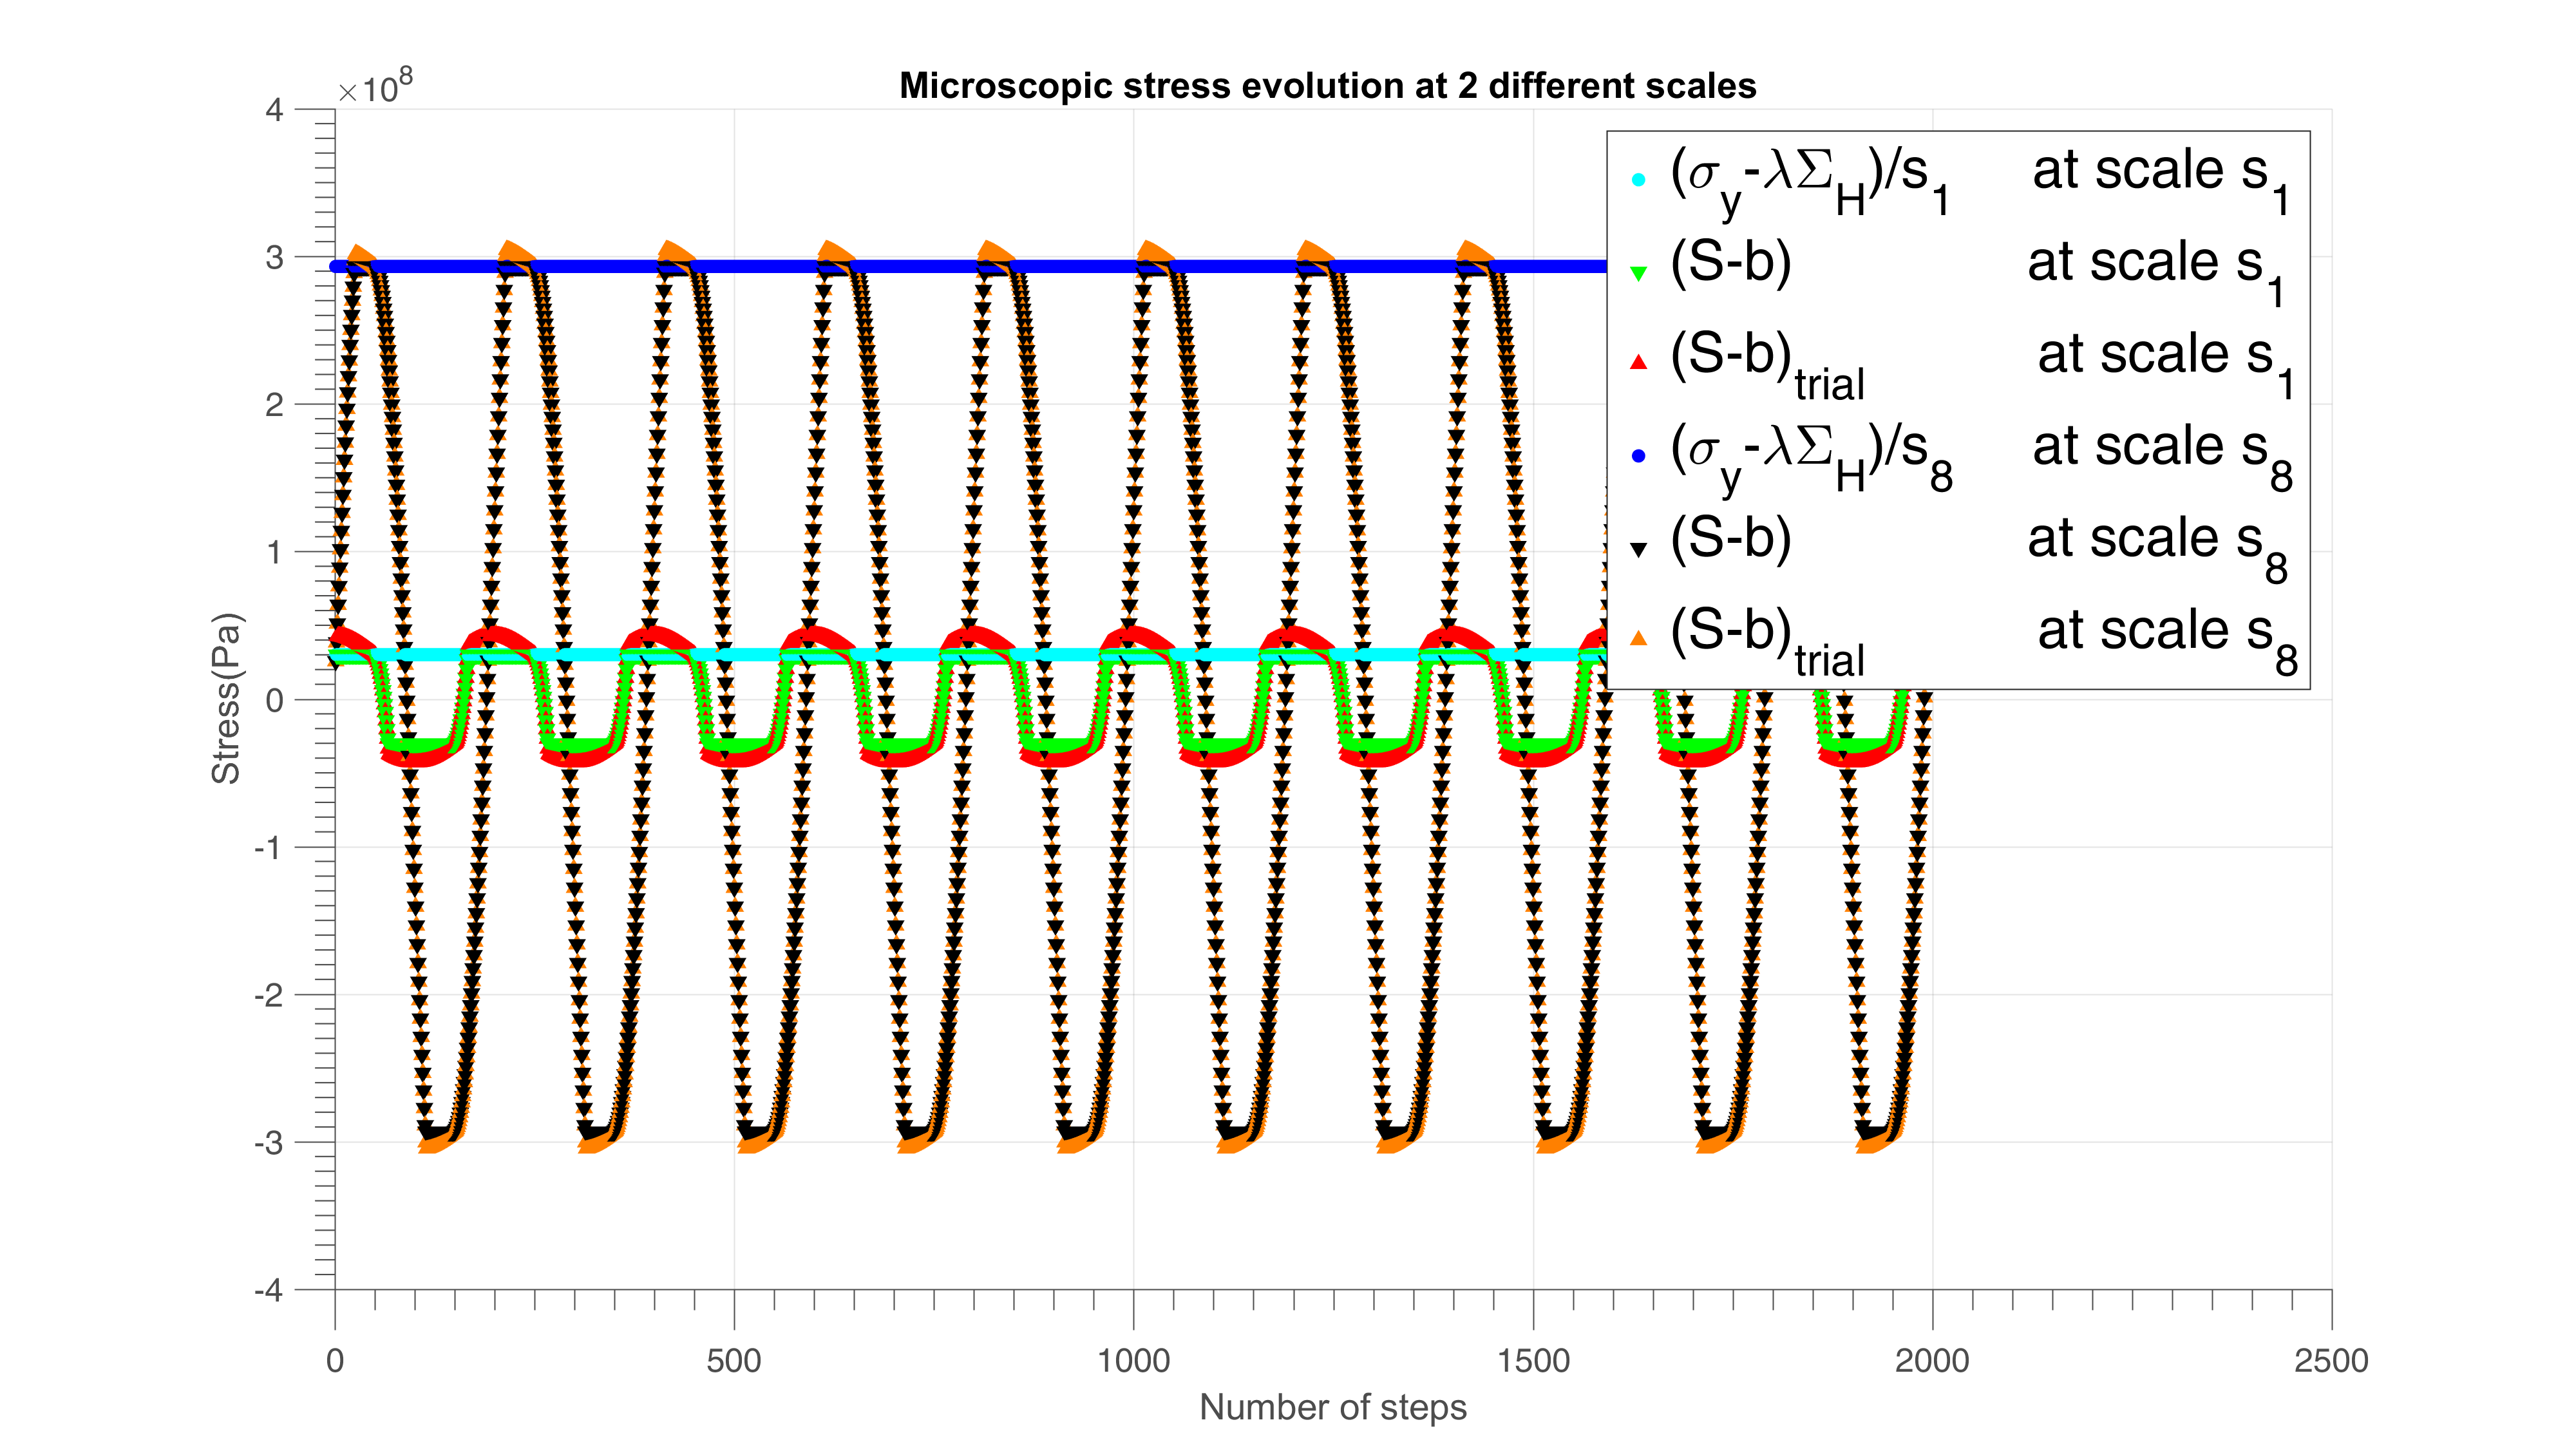
\includegraphics[width=\textwidth]{figures//trialsin.png} 
	\caption{Microscopic $\left(  \uline{\uline{S}}-\uline{\uline{b}}\right)_{trial}$ and $\left( \uline{\uline{S}}-\uline{\uline{b}}\right)$ evolution with time under different weakening scales in sinusoidal load}
	\label{trialsin}
\end{figure}

The damage evolves like in \figref{damsin}, where we compare the damage evolution as predicted by the cycle accumulation Eq.\eqref{eq:w} and by the numerical strategy of section 4.

\begin{figure}[!h]
	\centering
	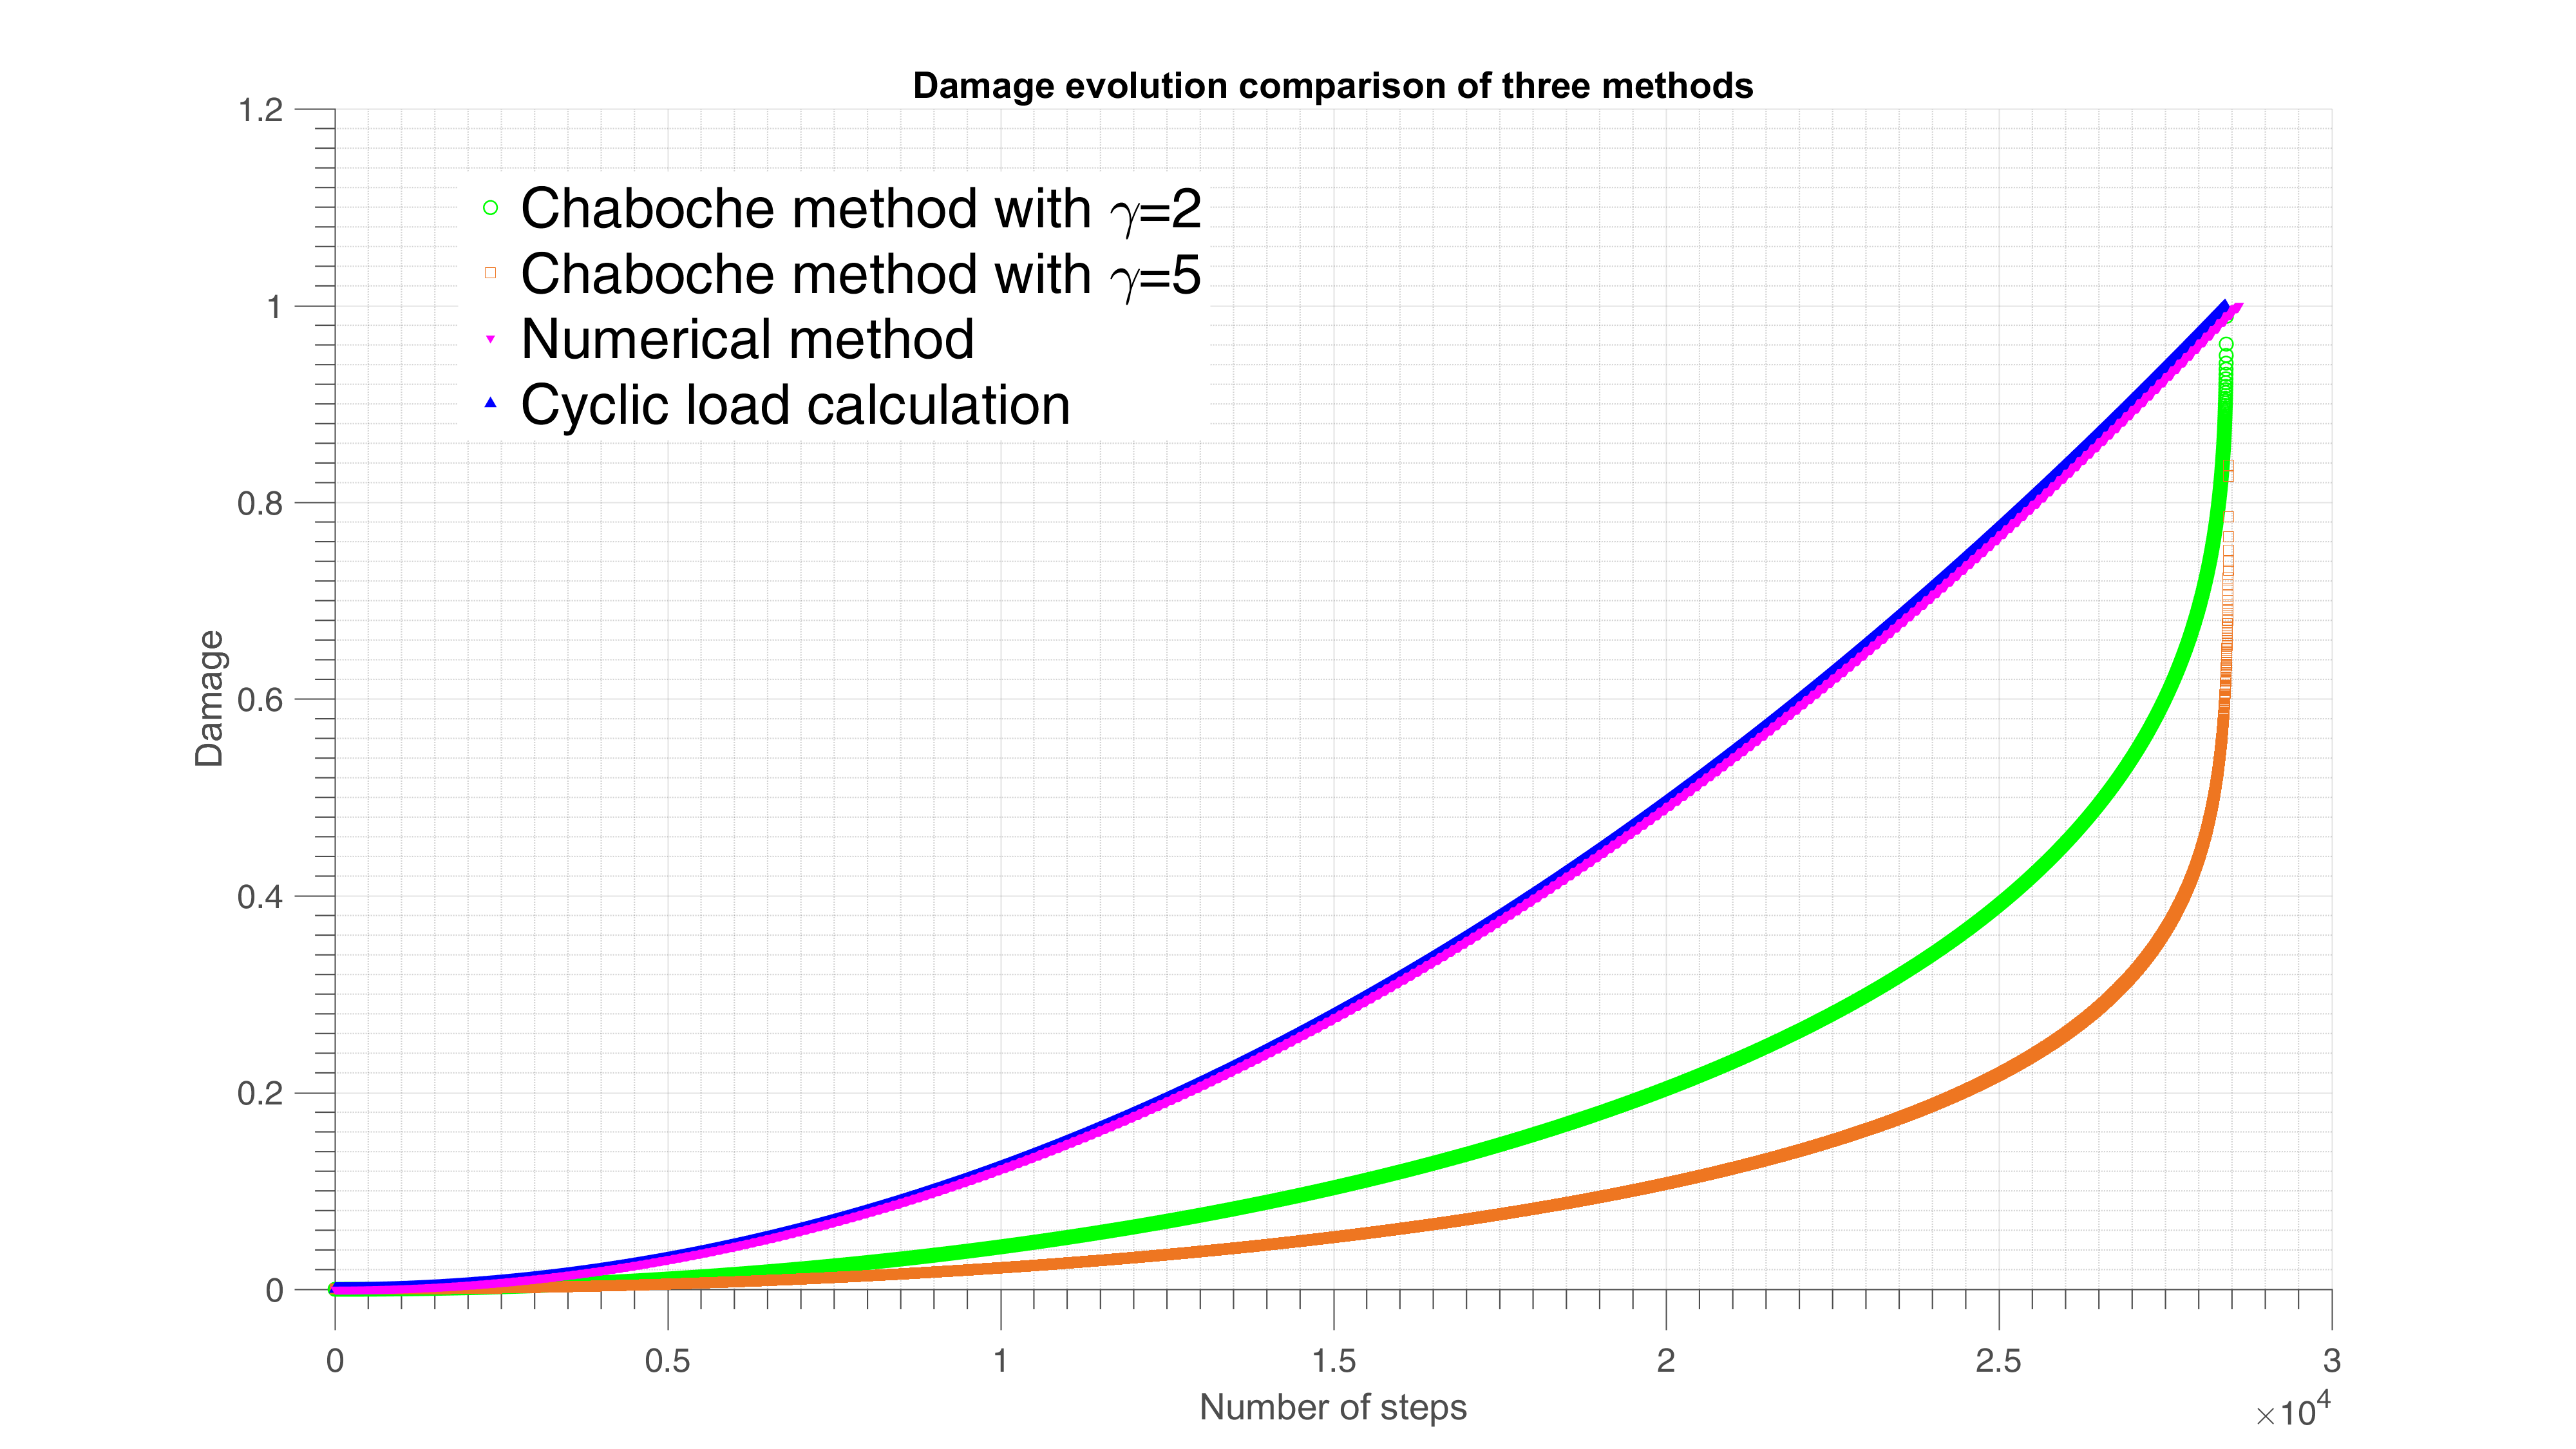
\includegraphics[width=\textwidth]{figures//damagesin.png} 
	\caption{Damage evolution with time under sinusoidal load with two different methods}
	\label{damsin}
\end{figure}

Now we compare the result to the one demonstrated in \figref{backstress}.  We can see from \figref{Damagediff}  the difference between cyclic load calculation and numerical method as function of time steps $n$. From the relative difference figure we conclude that the two methods converge.

\begin{figure}[!h]
	\centering
	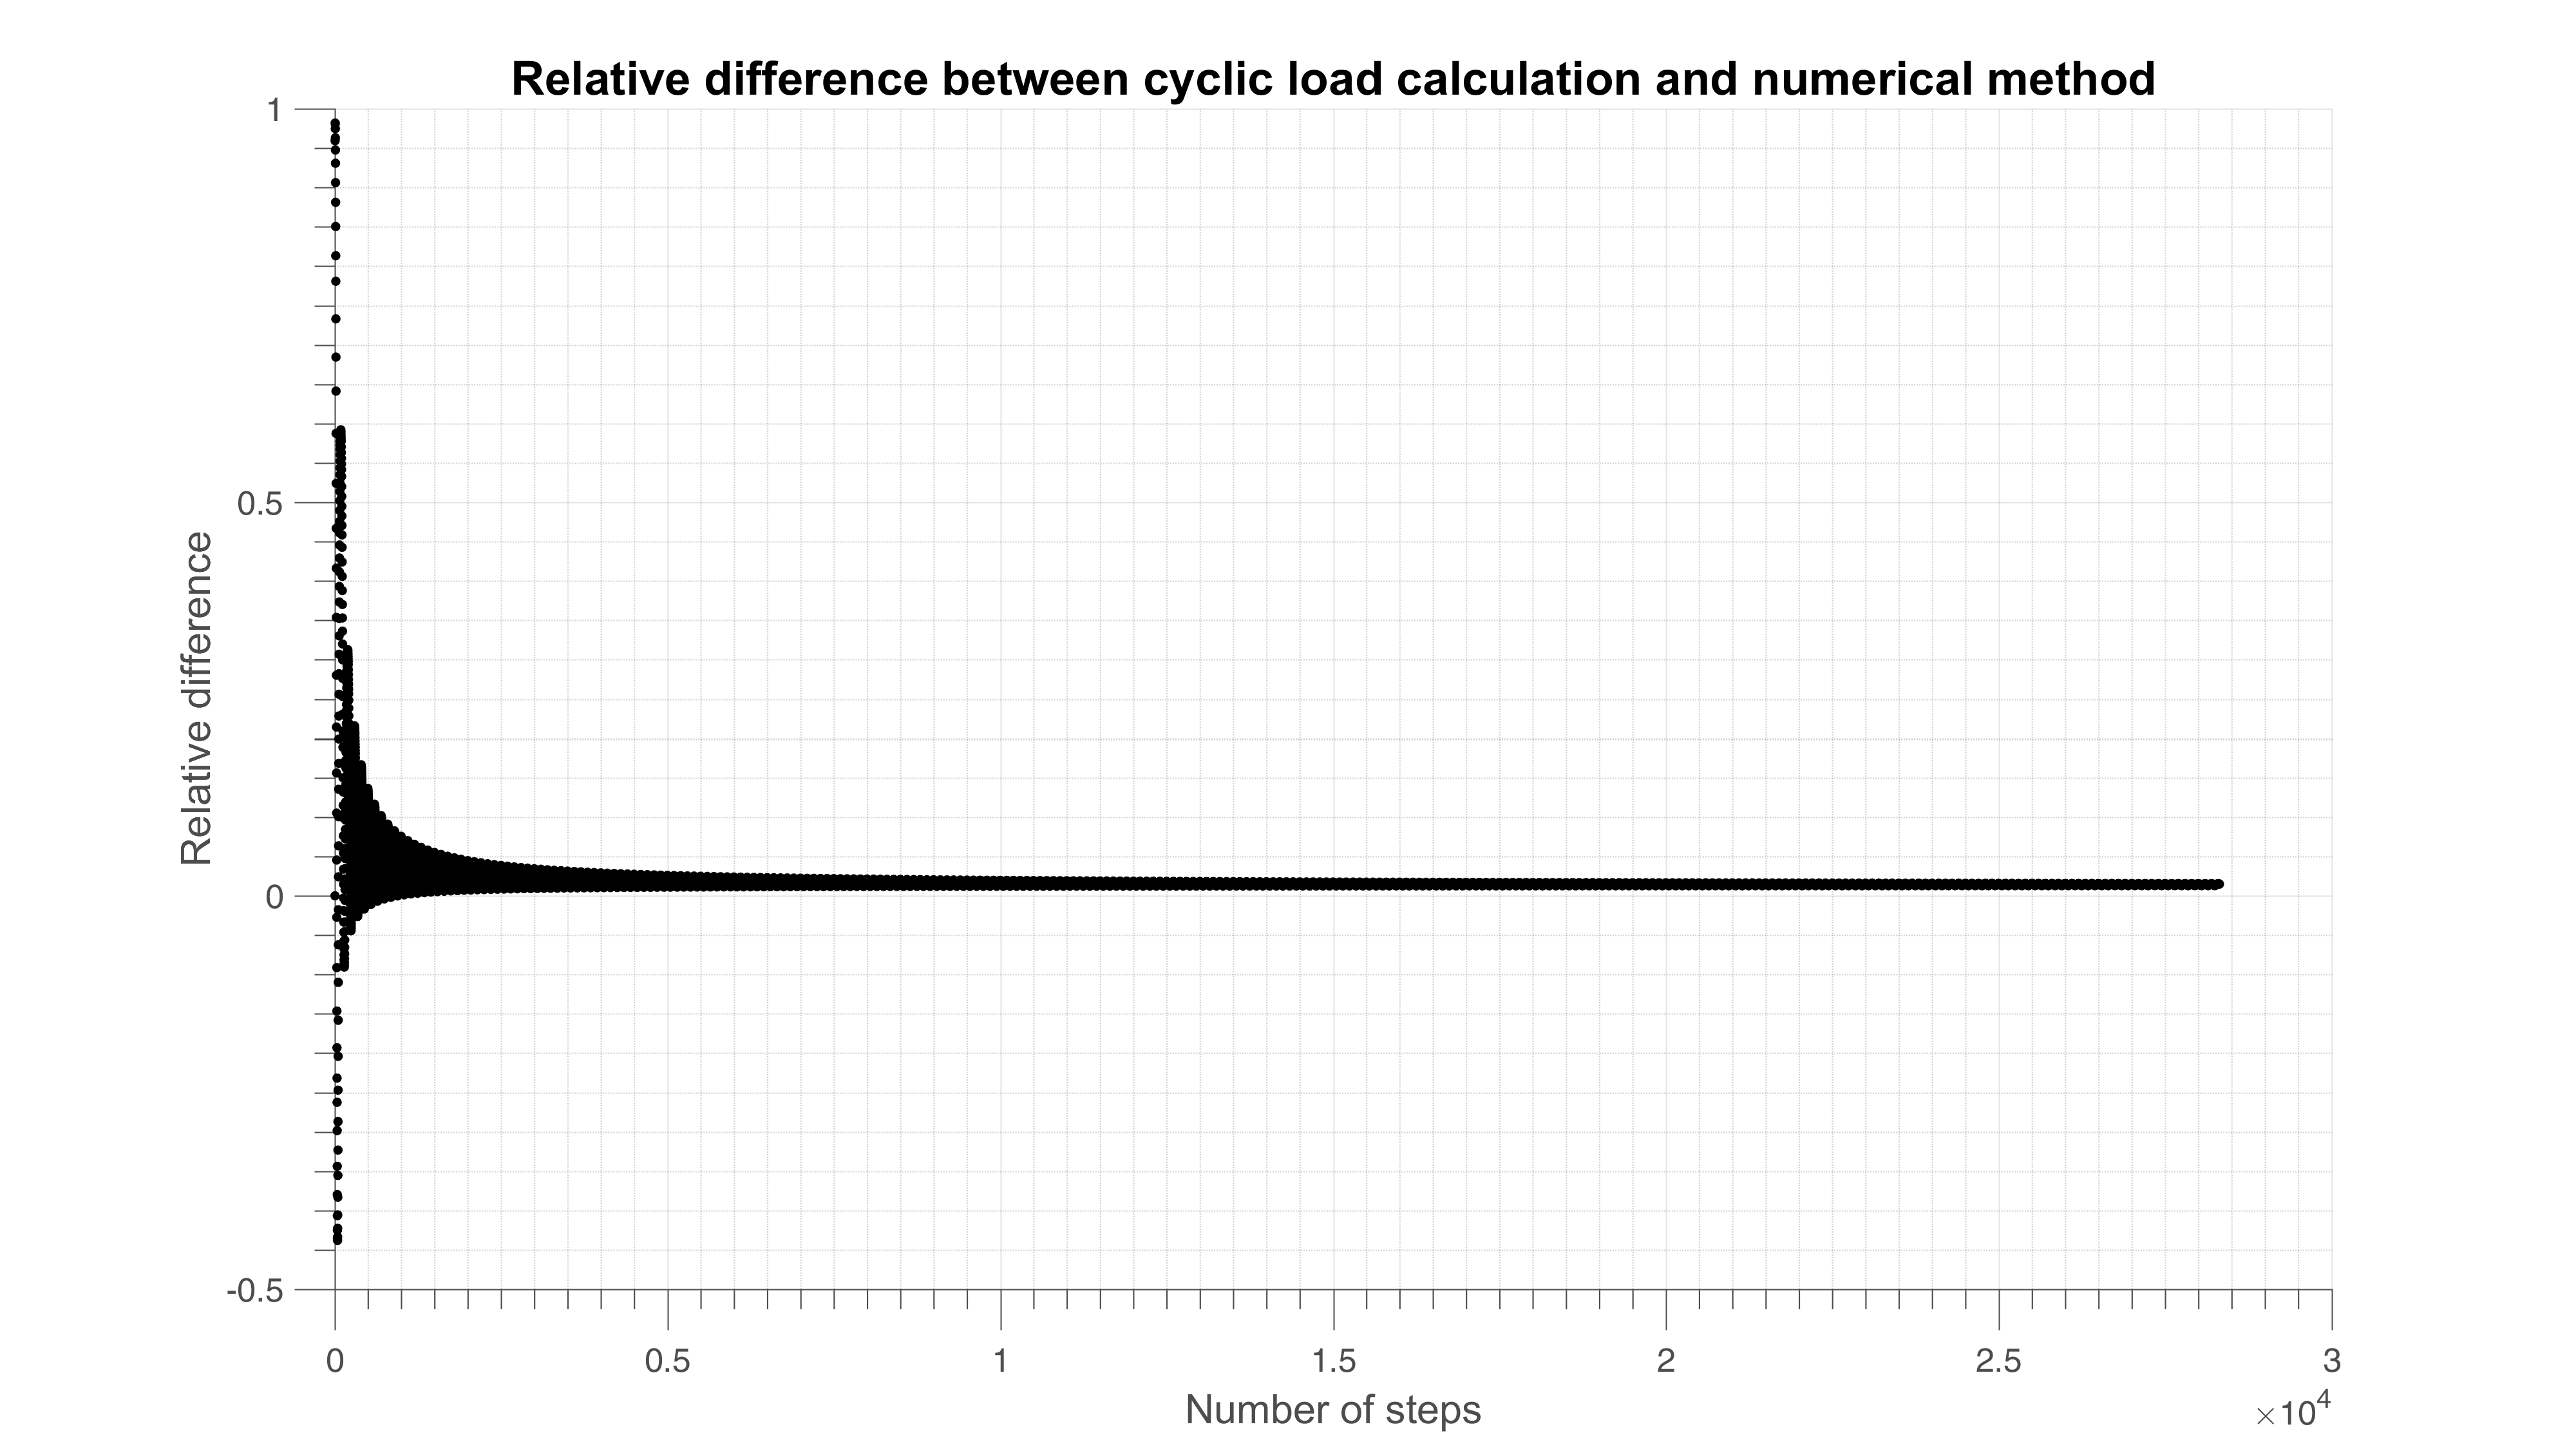
\includegraphics[width=0.8\textwidth]{figures//Damagediff.png} 
	\caption{$\dfrac{D_{analytical}-D_{numerical}}{D_{analytical}}$ evolution with time}
	\label{Damagediff}
\end{figure}

The cyclic load calculation is only valid for very simple such as proportional loading in fatigue, nevertheless it can still be used as a comparison group to verify the numerical results. The outcome seems satisfactory. Hence, to be more general for any loading history, we adopt the numerical method.

\newpage
\subsection{Recovery of sequence effect}
We adopt the parameter $\alpha$ to take into account the sequence effect. The high-low loading sequence clearly reduces the fatigue life, as depicted in \figref{sequence}. In order to cover this phenomenon, we let $\alpha$ change with time. Here $a$ is the sequence effect sensitivity.
$$s_{min}=\dfrac{\Sigma_y}{S_{max}}$$
which is the minimum weakening scale that activates energy loss.  We use a general law for $\alpha$ of the type $\alpha = \alpha (s_{min})$ with the idea that for us $s_{min}$ is a measure of present intensity of macroscopic stress = mechanical based stress norm. 


Numerically we review our method of the sequence effect as depicted in \figref{sequence}.
\begin{Figure}[h!]{Two level sequence effect.}[sequence]
\graphfile*[30]{figures//high-low-Smax.png}[]
\graphfile*[30]{figures//low-high-Smax.png}[]
\\
\graphfile*[30]{figures//high-low-D.png}[]
\graphfile*[30]{figures//low-high-D.png}[]
\label{sequence}
\end{Figure}


\clearpage
\section{Experimental verification}
\textbf{Comparison of fixed and varying $\alpha$ with constant amplitude loading}

The parameters we introduced during the deduction need to be calibrated. The source of the parameter identification are listed in Table.\ref{paras}.
In the case of constant amplitude loading, analytically $\alpha$ does not change with time because $S_{max}$ is a linear function of stress intensity. However, numerically $\alpha$ changes with time because real life experiments have fluctuations. The comparison with the average $\alpha$ are shown in \figref{fig:alpha}. The relative error of number of points to failure is 0.259\%.

\begin{figure}[!h]
	\centering
	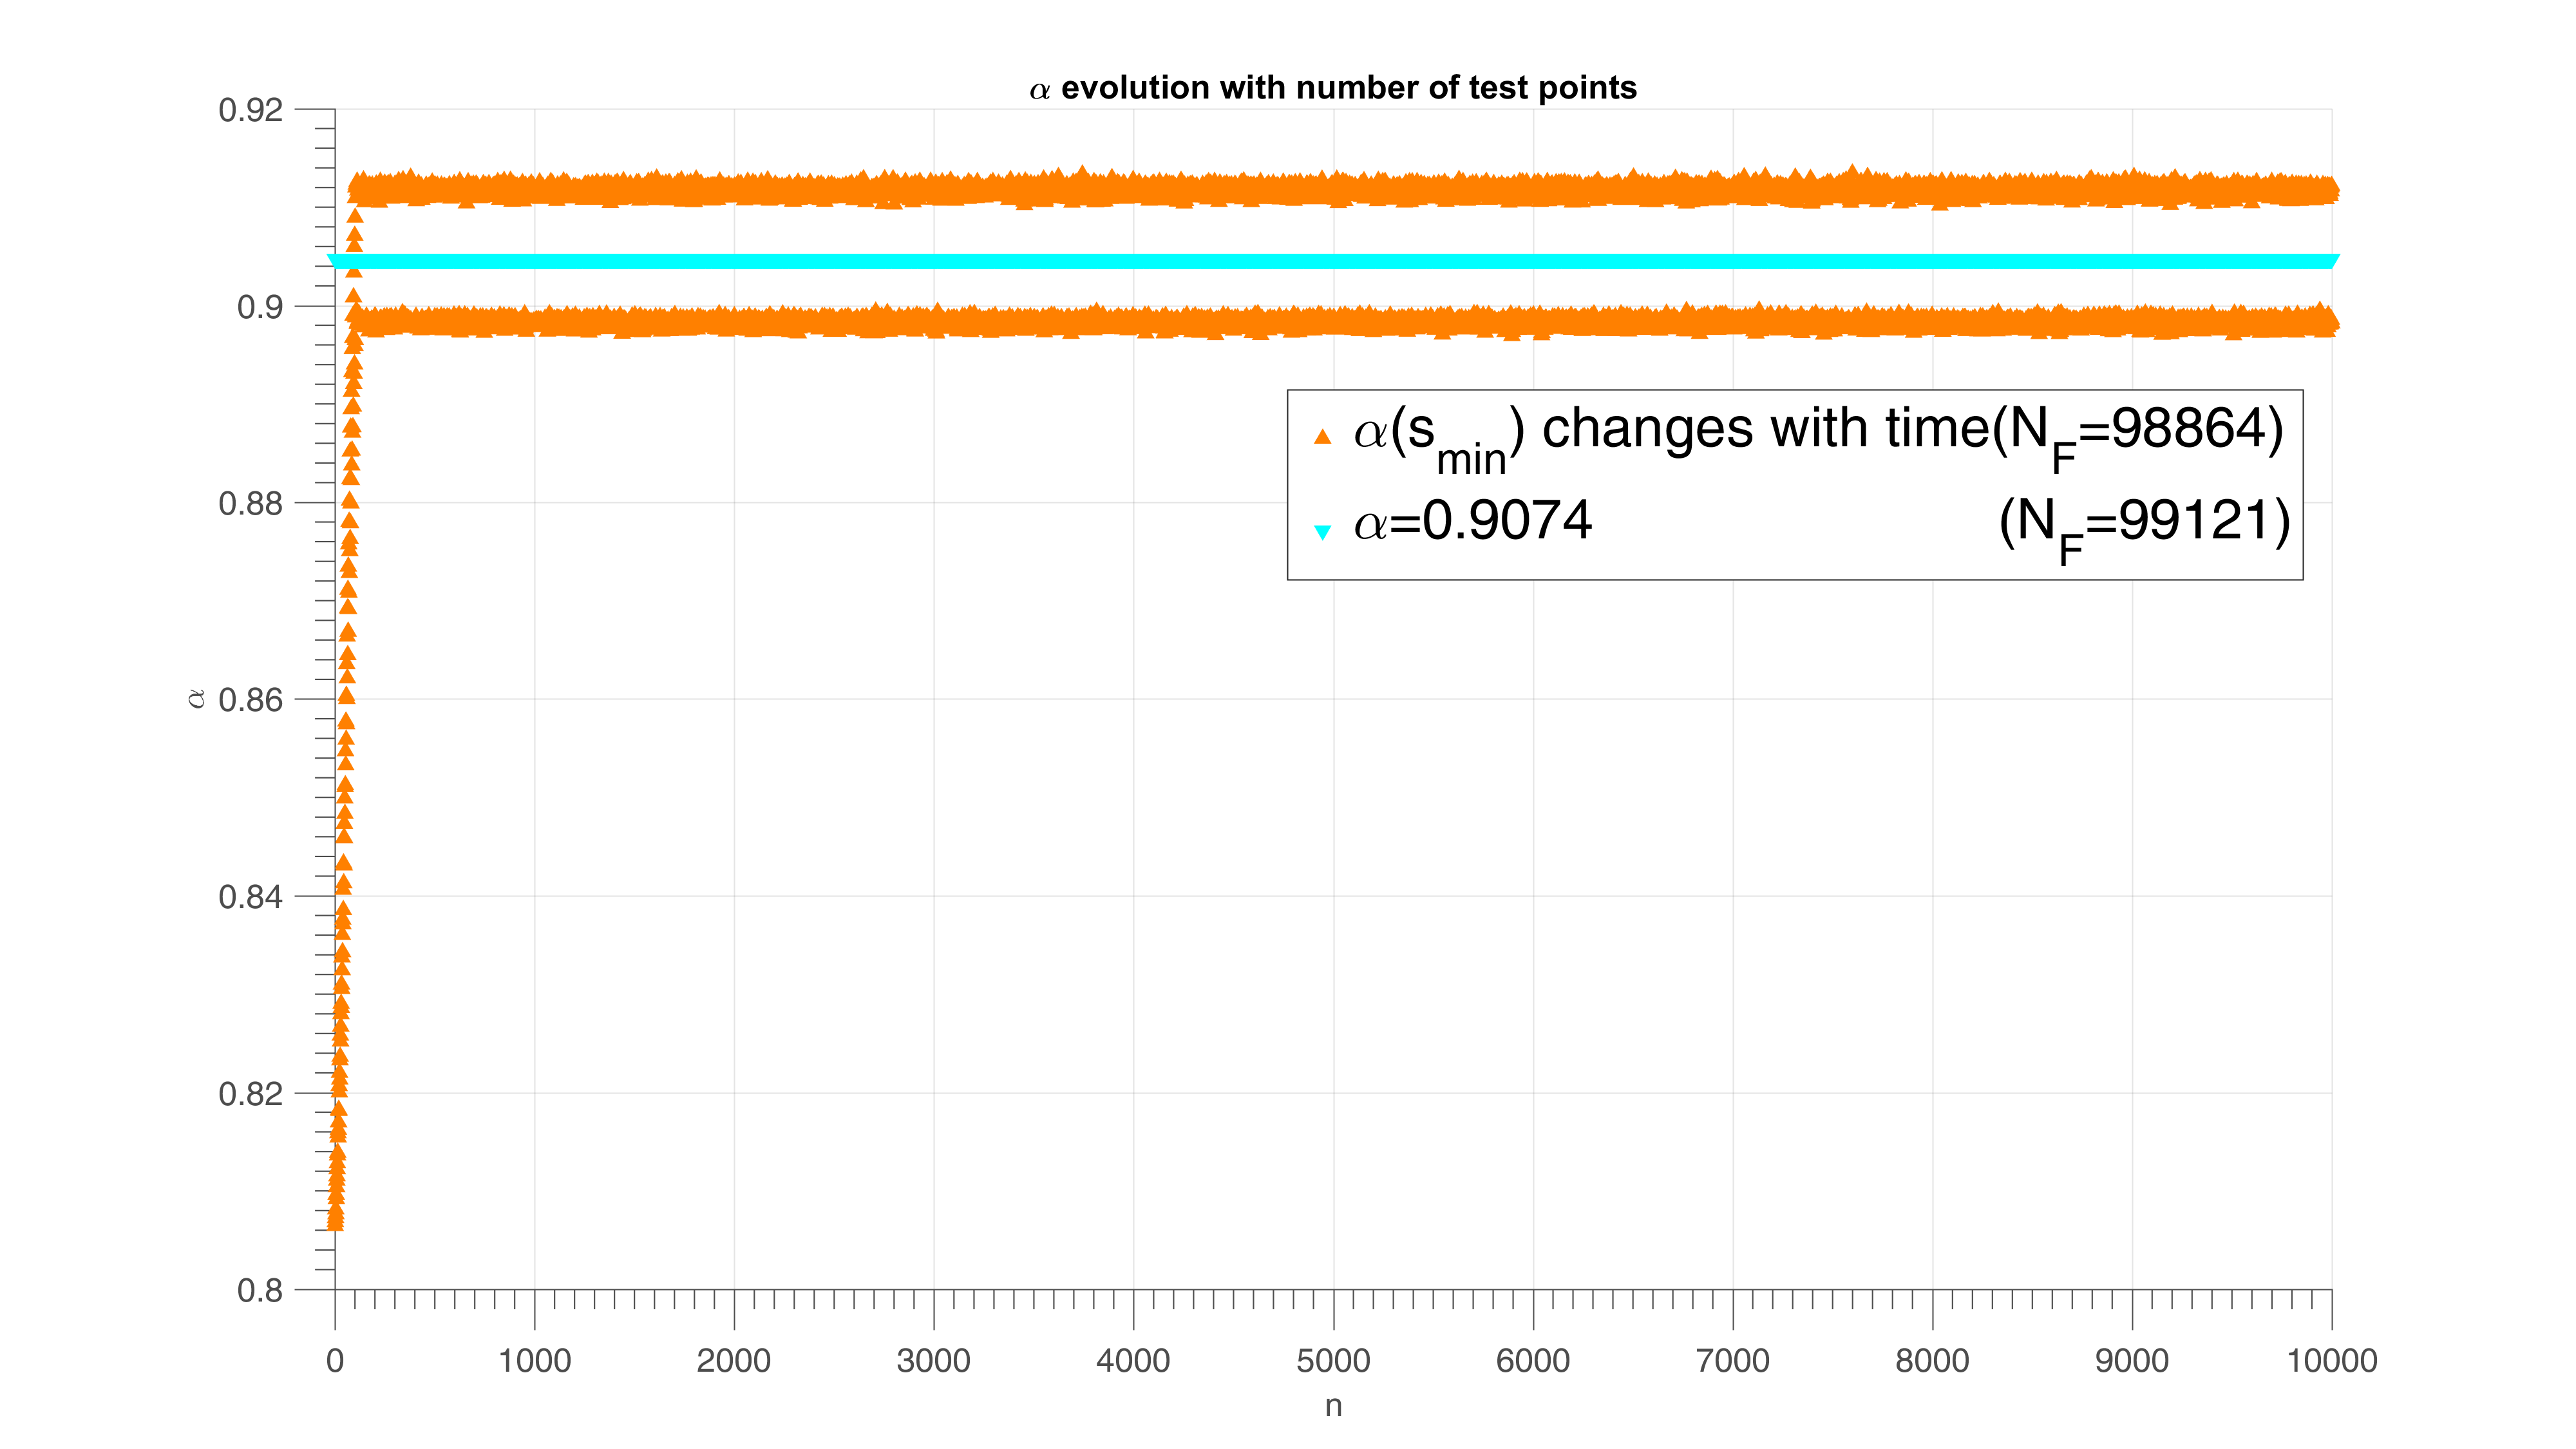
\includegraphics[width=\textwidth]{figures//alpha_change_with_time.png} 
	\caption{Different choice of alpha numerically}
	\label{fig:alpha}
\end{figure}


\begin{table}[!h]
	\centering
	\begin{tabular}{l|c}
		\hline
		\textbf{Parameters}                                  & \multicolumn{1}{c}{\textbf{Strategy}} \\ \hline
		Hardening parameter k                                & material constant                      \\
		Macroscopic yield stress $\sigma_y$                  & material constant                      \\
		Hydrostatic pressure sensitivity $\lambda$           & hydrostatic stress sensitivity         \\
		Non-linearity of damage accumulation  $a$        & amplification factor of load intensity      \\
		Weakening scales distribution exponent  $\beta$      & to be calibrated                          \\
		Dissipated energy to failure per defect  $W_0$ & energy scaling               \\ \hline
	\end{tabular}
	\caption{Parameters concerned}
\label{paras}
\end{table}

\subsection{Constant amplitude 1D tests from Cetim}

The tests are performed on aluminum batches, the characteristics of the sample are shown in table.\ref{tab:cetim}.
\begin{figure}[!h]
	\centering
	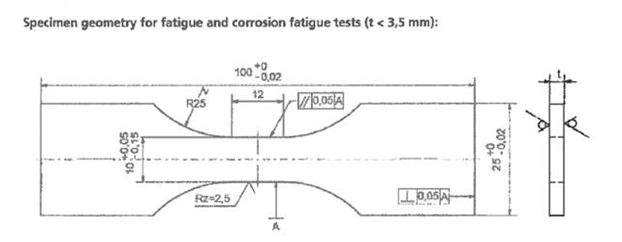
\includegraphics[width=0.7\textwidth]{figures//aluminum_cetim.png} 
	\caption{Specimen geometry for fatigue tests of aluminum}
	\label{fig:aluminum}
\end{figure}
\begin{table}[!h]
	\centering
	\begin{tabular}{ll}
		\hline
		\textbf{Parameters}                                         & \textbf{Value}                    \\ \hline
		Young's modulus                                             & $E=72$ GPa                       \\
		Hardening parameter                                         &  $k=6$ MPa \\
		Macroscopic yield stress                                    & $\sigma_y=230$ MPa              \\
		Thickness & $e=2.9mm$                        \\
		Width		 & $l= 9.95mm$                        \\ \hline
	\end{tabular}
	\caption{Material parameters}
	\label{tab:cetim}
\end{table}



\newpage
\subsection{Random amplitude 1D tests from Cetim}

\textbf{Parameter sensitivity analysis}

The tests on uniaxial loading of a certain material needs a fixed set of parameters. We first perform a sensitivity analysis to see the influence of each parameter. We analyze the sensitivity of parameters separately as in Table.\ref{sensitivity}. 

In Miner's law the parameter $\alpha$ is zero, the maximum value is below 1. For $\alpha=1$ the damage accumulation line becomes flat and there is unlimited lifetime. To keep $\alpha$ in the range of $\{0,1\}$ where in random amplitude tests there is $S_{max}=163.3MPa$. We have $a$ ranging from $0.1$ to $0.29$ when $X=1$ and $f(\beta)=1$. 
To assess large stress correctly we define the larger stress intensity as: 
$$S_{large}>\dfrac{X\Sigma_y}{2}.$$ 
So here $X$ ranges from $0.5$ to $2$. The weakening scale distribution exponent $\beta$ ranges from $1$ to $5$. $\gamma$ is  material parameter from Chaboche law related to extremity of damage accumulation so we give it ranging from $0.01$ to $3$, here we use $0.1$ to keep $\alpha$ positive. The hydrostatic pressure sensitivity $\lambda$ is from positive mean stress test, which has the range of $0\sim0.8$. In constant amplitude cyclic loading, the dissipated energy to failure per defect $W_0/n_0$ is related to fatigue lifetime of the material.


\begin{table}[]
	\centering
	\begin{tabular}{l|rrr|rrr|r}
		\hline
		\textbf{Parameter}        & \textbf{Ref} & \textbf{Min} & \textbf{Max} & \textbf{Ref\_n} & \textbf{Min\_n} & \textbf{Max\_n} & \textbf{Sensitivity} \\ \hline
		\textbf{$\beta$}          & 1.5                      & 1.40         & 1.60         & 97194                 & 94806           & 102862          & 0.62                 \\
		\textbf{$\gamma$}         & 0.1                        & 0.05         & 0.2         & 97194                 & 109866          & 87583           & -0.80                \\
		\textbf{$\lambda$}        & 0.3                      & 0.20         & 0.40         & 97194                 & 103144          & 89499           & -0.21                \\
		\textbf{$W_0/n_0$}        & 1E8                      & 9E7          & 1.1E8        & 97194                 & 88673           & 106485          & 0.92                 \\
		\textbf{$a$}              & 0.1                      & 0.08         & 0.12         & 97194                 & 115515          & 83739           & -0.82                \\
		\textbf{$X$}              & 1                        & 0.90         & 1.10         & 97194                 & 63170           & 118781          & 2.86                 \\
		\textbf{$f(\beta)$} & 1                        & 0.90         & 1.10         & 97194                 & 100583          & 93287           & -0.38                \\ \hline
	\end{tabular}
	\caption{Parameters sensitivity at random loading}
	\label{sensitivity}
\end{table}
The sensitivity of parameters is calculated with Eq.\eqref{eq.sensitivity}.
\begin{equation}
sensitivity = \dfrac{\left( Max_n-Min_n\right)/Ref_n}{\left( Max-Min\right)/Ref}.
\label{eq.sensitivity}
\end{equation}

There are 12 validated uniaxial fatigue tests on the aluminum sample, in which 2 are constant amplitude load case and 10 random  load case. 
The cyclic stress of test number 1(ep01) and test number 2(ep02) are respectively $131.9MPa$ and $97.0MPa$. We first identify the same parameters feasible to both loading cases. We find when $\beta=1.5$ the constant cyclic load case has the same relative error.

	\begin{figure}[!h]
	\centering
	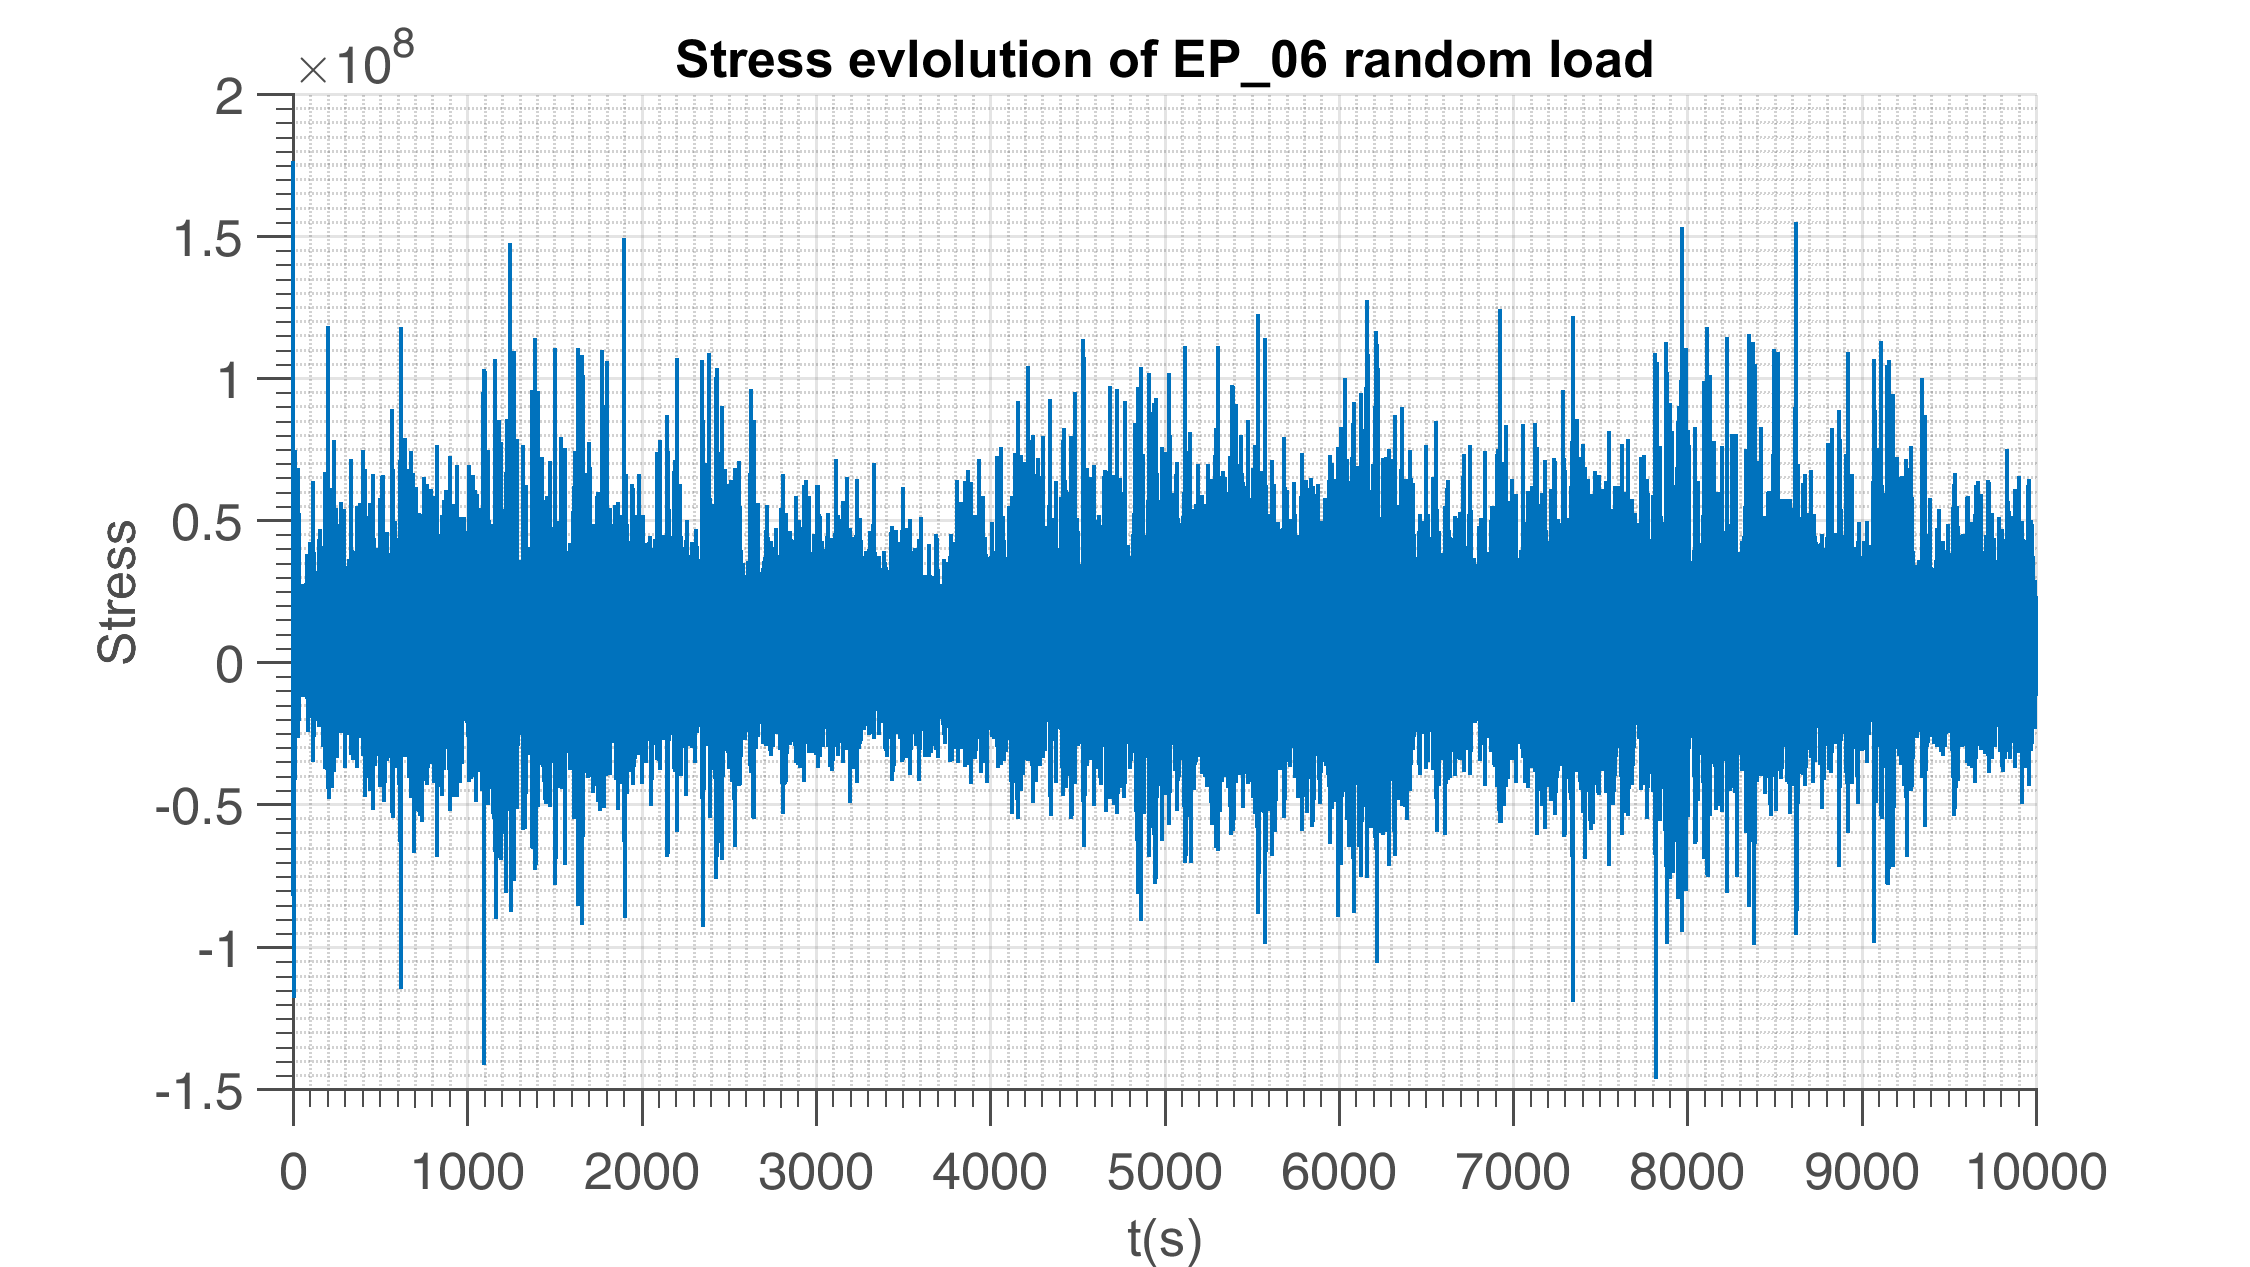
\includegraphics[width=\textwidth]{figures//ep_06_stress.png} 
	\caption{Random loading history on batch 06}
\end{figure}	
The detailed tests information are shown in table.\ref{tab:Cetim}. There are 27000($\pm 2.4\%$) recorded points per repetition. 

\begin{table}[!h]
	\centering
	\begin{tabular}{lllll}
		\hline
		\textbf{Specimen} & \textbf{Fmax (kN)} & \textbf{$\Sigma_{max}$ in the block} & \textbf{Number of repetition} & \textbf{Number of points} \\ \hline
		BATCH\_A\_01      & 3.375              &                                      &                                          & 99892                                \\
		BATCH\_A\_02      & 2.475              &                                      &                                          & 414298                               \\
		BATCH\_A\_04      & nom                & 225.88                               & 95                                       & 2500000                              \\
		BATCH\_A\_05      & nom                & 225.88                               & 156                                      & 4105263                              \\
		BATCH\_A\_06      & nom                & 225.88                               & 145                                      & 3815789                              \\
		BATCH\_A\_07      & nom                & 225.88                               & 90                                       & 2368421                              \\
		BATCH\_A\_08      & nom                & 225.88                               & 194                                      & 5105263                              \\
		BATCH\_A\_09      & nom                & 225.88                               & 197                                      & 5184211                              \\
		BATCH\_A\_10      & nom x 0,9          & 203.292                              & 515                                      & 13552632                             \\
		BATCH\_A\_11      & nom x 0,9          & 203.292                              & 385                                      & 10131579                             \\
		BATCH\_A\_12      & nom x 0,9          & 203.292                              & 424                                      & 11157895                             \\
		BATCH\_A\_13      & nom x 0,9          & 203.292                              & 409                                      & 10763158                             \\ \hline
		BATCH\_B\_01      & nom                & 225.88                               & 121                                      & 3184211                              \\
		BATCH\_B\_02      & nom x 0,8          & 180.704                              & 380                                      & 10000000                             \\
		BATCH\_B\_03      & nom x 0,8          & 180.704                              & 380                                      & 10000000                             \\
		BATCH\_B\_04      & nom x 0,9          & 203.292                              & 406                                      & 10684211                             \\
		BATCH\_B\_05      & nom x 0,9          & 203.292                              & 454                                      & 11947368                             \\
		BATCH\_B\_06      & nom x 0,9          & 203.292                              & 518                                      & 13631579                             \\
		BATCH\_B\_07      & nom x 0,9          & 203.292                              & 553                                      & 14552632                             \\
		BATCH\_B\_08      & nom x 0,9          & 203.292                              & 612                                      & 16105263                             \\
		BATCH\_B\_09      & nom                & 225.88                               & 253                                      & 6657895                              \\
		BATCH\_B\_10      & nom                & 225.88                               & 196                                      & 5157895                              \\
		BATCH\_B\_11      & nom                & 225.88                               & 178                                      & 4684211                              \\
		BATCH\_B\_12      & nom                & 225.88                               & 123                                      & 3236842                              \\ \hline
	\end{tabular}
	\caption{Cetim fatigue tests result on 2 batches}
\label{tab:Cetim}
\end{table}

We assume the material parameters like Young's modulus, hardening parameter, hydrostatic pressure sensitivity, macroscopic yield stress, Wohler curve exponent and sequence effect parameters are known. We first identify the weakening scales distribution, and dissipated energy to failure from cyclic tests ep01 and ep02. Then change the parameter $n_0$ to see if our assumption is correct or need to be changed. 

To see the influence of sequence effect factor of $\alpha$, we first fix $\alpha=0.65462$ for all tests to see the results. We find out that the fatigue life of random loading is widely dispersed. In this case we need to use $\alpha=f(s_{min})$ which evolves with time to make large stress intensity deal more damage.

The $\alpha$ parameter has crucial influence on the damage accumulation on different stress intensities. In \figref{fig.alpha} we can see $\alpha$ value and damage accumulation speed as function of life proportion. The range of $\alpha$ is $[-\infty,1]$ but the negative values of $\alpha$ lost its physical meaning for the damage accumulation becomes slower at the later stage of fatigue.
From Eq.\eqref{eqD} we can draw the evolution of damage with different $\alpha$ to see its influence on the accumulation law.
\begin{figure}[!h]
	\centering
	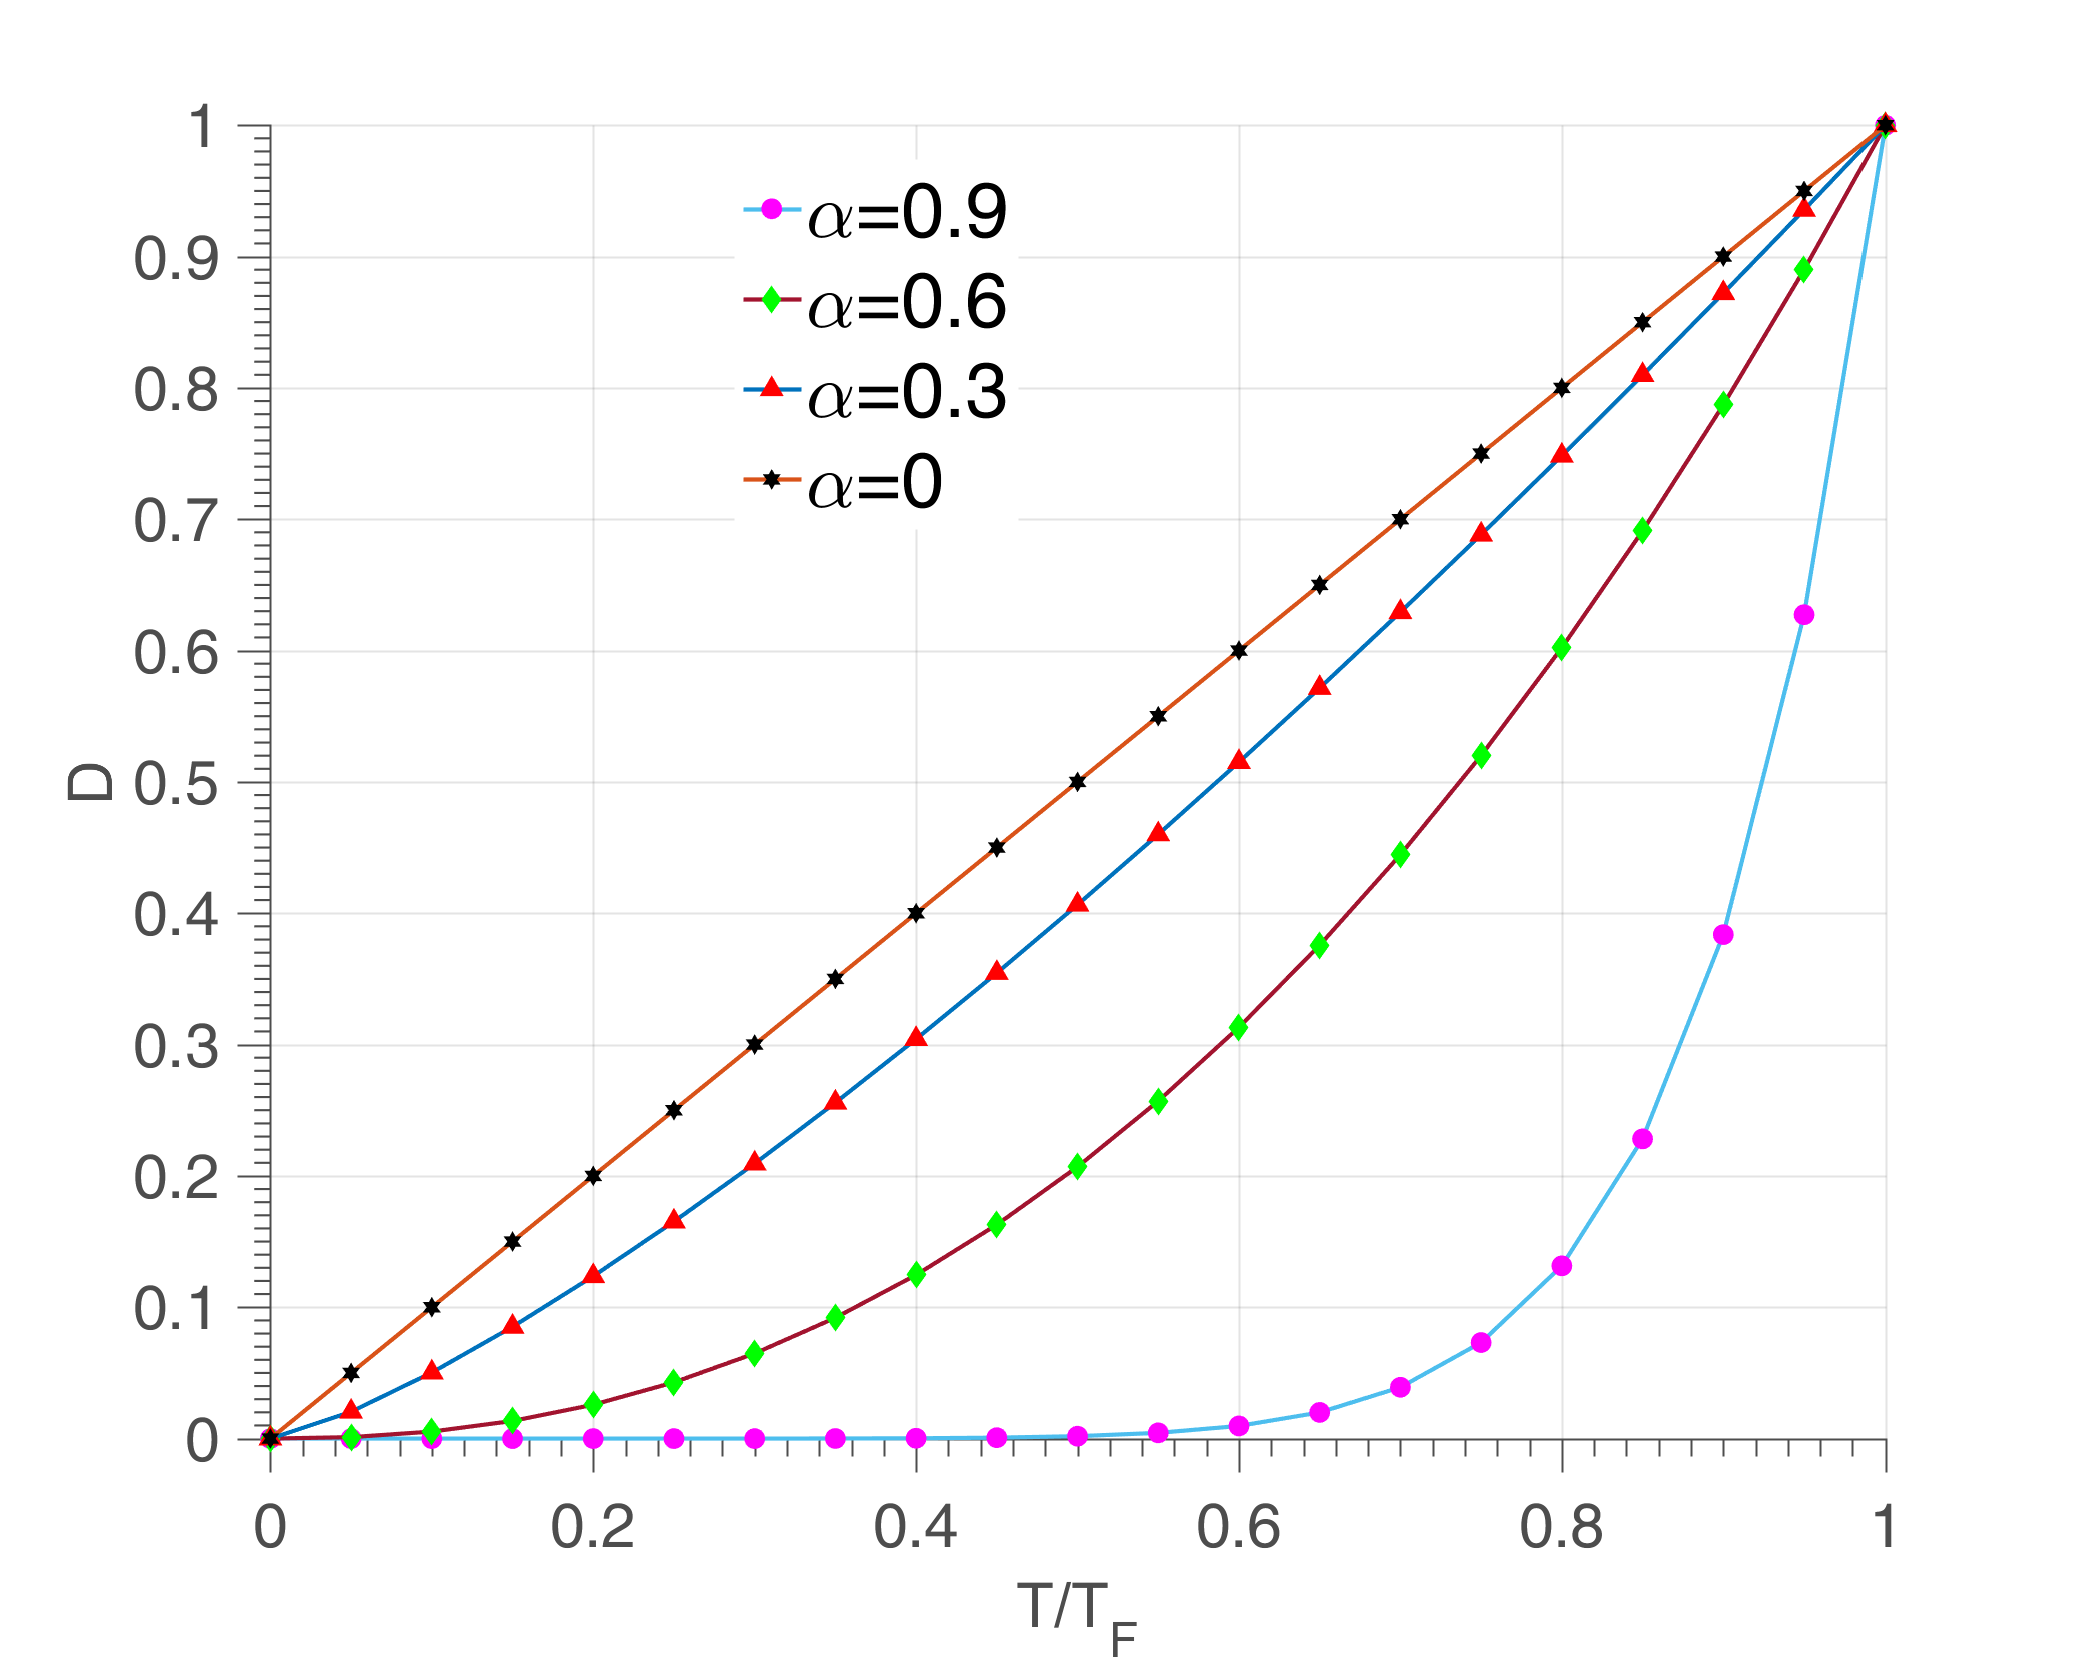
\includegraphics[width=\textwidth]{figures//alpha.png} 
	\caption{Influence of $\alpha$ on damage accumulation with $\gamma=0.1$}
	\label{fig.alpha}
\end{figure}

The numerical fitting process show that the damage is caused mainly by large stresses. The definition of major stress now need to be specified according to the material. To take into account this effect we first find out the proportion stress above a certain value in the repetition signal of random loading, as shown in Table.\ref{tab.majordamage}.  Here ep\_a and ep\_b are the same material. Since the samples were extracted from aluminum profiles of industrial production,  the two batches only  correspond to two different times of sampling in the production. The variation is supposed to be representative of the regular tolerances you might have in the production. ep\_a\_01 and ep\_a\_02 are constant amplitude loading which helps identify the power of weakening scale distribution $\beta$. ep\_a\_03 is low cycle fatigue data.  ep\_b\_01 and ep\_b\_02 have infinite life time. The data in the table are grabbed from random signal high cycle fatigue loading history.

\begin{table}[!h]
	\centering
	\begin{tabular}{llllllll}
		\hline
		\textbf{Stress\textgreater}  & \textbf{70}    & \textbf{90}    & \textbf{110}   & \textbf{130}    & \textbf{150}    & \textbf{170}    & \textbf{190}    \\
		\textbf{$S_{max}$\textgreater} & \textbf{57.15} & \textbf{73.48} & \textbf{89.81} & \textbf{106.14} & \textbf{122.47} & \textbf{138.80} & \textbf{155.13} \\
		\textbf{$X$}                 & \textbf{0.497} & \textbf{0.639} & \textbf{0.781} & \textbf{0.923}  & \textbf{1.065}  & \textbf{1.207}  & \textbf{1.349}  \\ \hline
		\textbf{ep\_a\_04}           &                & 1.962\%        & 0.904\%        & 0.077\%         & 0.037\%         & 0.018\%         & 0.007\%         \\
		\textbf{ep\_a\_05}           &                & 1.604\%        & 0.784\%        & 0.044\%         & 0.030\%         & 0.007\%         & 0.007\%         \\
		\textbf{ep\_a\_06}           &                & 1.645\%        & 0.784\%        & 0.045\%         & 0.030\%         & 0.007\%         & 0.007\%         \\
		\textbf{ep\_a\_07}           &                & 1.632\%        & 0.788\%        & 0.048\%         & 0.029\%         & 0.007\%         & 0.007\%         \\
		\textbf{ep\_a\_08}           &                & 1.644\%        & 0.787\%        & 0.048\%         & 0.037\%         & 0.007\%         & 0.007\%         \\
		\textbf{ep\_a\_09}           &                & 1.655\%        & 0.800\%        & 0.048\%         & 0.037\%         & 0.007\%         & 0.007\%         \\
		\textbf{ep\_a\_10}           &                & 0.768\%        & 0.134\%        & 0.007\%         & 0.000\%         & 0.000\%         & 0.000\%         \\
		\textbf{ep\_a\_11}           &                & 0.772\%        & 0.145\%        & 0.007\%         & 0.000\%         & 0.000\%         & 0.000\%         \\
		\textbf{ep\_a\_12}           &                & 0.779\%        & 0.133\%        & 0.011\%         & 0.000\%         & 0.000\%         & 0.000\%         \\
		\textbf{ep\_a\_13}           &                & 0.775\%        & 0.141\%        & 0.007\%         & 0.000\%         & 0.000\%         & 0.000\%         \\ \hline
		\textbf{ep\_b\_01}           & 4.739\%        & 1.737\%        & 0.840\%        & 0.224\%         & 0.049\%         & 0.034\%         & 0.004\%         \\
		\textbf{ep\_b\_04}           & 1.999\%        & 0.745\%        & 0.156\%        & 0.034\%         & 0.004\%         & 0.000\%         & 0.000\%         \\
		\textbf{ep\_b\_05}           & 2.010\%        & 0.749\%        & 0.148\%        & 0.034\%         & 0.008\%         & 0.000\%         & 0.000\%         \\
		\textbf{ep\_b\_06}           & 1.999\%        & 0.790\%        & 0.118\%        & 0.034\%         & 0.008\%         & 0.000\%         & 0.000\%         \\
		\textbf{ep\_b\_07}           & 2.029\%        & 0.756\%        & 0.152\%        & 0.034\%         & 0.008\%         & 0.000\%         & 0.000\%         \\
		\textbf{ep\_b\_08}           & 1.999\%        & 0.737\%        & 0.137\%        & 0.034\%         & 0.008\%         & 0.000\%         & 0.000\%         \\
		\textbf{ep\_b\_09}           & 4.663\%        & 1.687\%        & 0.798\%        & 0.205\%         & 0.049\%         & 0.034\%         & 0.004\%         \\
		\textbf{ep\_b\_10}           & 4.712\%        & 1.744\%        & 0.809\%        & 0.224\%         & 0.046\%         & 0.034\%         & 0.004\%         \\
		\textbf{ep\_b\_11}           & 4.636\%        & 1.664\%        & 0.790\%        & 0.209\%         & 0.049\%         & 0.034\%         & 0.004\%         \\
		\textbf{ep\_b\_12}           & 0.775\%        & 0.141\%        & 0.007\%        & 0.000\%         & 0.000\%         & 0.000\%         & 0.000\%         \\ \hline
	\end{tabular}
	\caption{Proportion of major damage stress applied(MPa) where $\Sigma_y$=230MPa, data provided by Cetim.}
	\label{tab.majordamage}
\end{table}

\clearpage
\textbf{Major damage effect}

With the new $\alpha$ we are able to calibrate our model better with the experimental results. 
$$\alpha=1-a\left\langle \dfrac{\frac{1}{s_{min}}}{X-\frac{1}{s_{min}}} \right\rangle^{f(\beta)}.$$
$f(\beta)$ decreases when $\beta$ increases, because less weakening scale activation leads to less damage. 

For instance in constant amplitude loading, the number of cycles to failure according to Eq.\eqref{eq.NFWcyc} is expressed as Eq.\eqref{eq.nf}:
\begin{equation}
\begin{split}
N_F&=\dfrac{W_0}{\left( 1-\alpha\right)W_{cyc} }
\\&=\dfrac{W_0}{\left( 1-\alpha\right)C_1}S_{max}^{-\beta-1}
\\&= \frac{W_0}{a\left\langle \dfrac{\frac{1}{s_{min}}}{1-\frac{1}{s_{min}}} \right\rangle^\beta}\dfrac{E(E+k\nu)\beta\left( \beta+1\right) }{ 4(E-k)(1+\nu)\left( \beta-1\right) }\dfrac{\left(\sigma_y-\lambda \Sigma_H\right)^{\beta-1}}{S_{max}^{\beta+1} }  .
\end{split}
\label{eq.nf}
\end{equation}


The influence of all the parameters are shown in \figref{fig.para}. The standard S-N curve is fitted with fatigue data provided by Cetim(the red line and value in Tab.\ref{tab.cetim.para}).

\begin{table}[!h]
	\centering
	\begin{tabular}{rrrrrrrr}
		\hline
		\textbf{Parameter} & \textbf{$W_0$} & \textbf{$\lambda$} & \textbf{$\beta$} & \textbf{$S_{large}>$} & \textbf{$X$} & \textbf{$a$} & \textbf{$f(\beta)$} \\
		\textbf{Value}     & 5.58e8         & 0.1                & 1.5              & 122                  & 1.065        & 0.1          & 1.4                 \\ \hline
	\end{tabular}
	\caption{The parameters in 1D cyclic and random loading on aluminum fatigue tests by Cetim}
	\label{tab.cetim.para}
\end{table}

\begin{Figure}[!h]{The influence of parameters on the shape and limit of S-N curve}[fig.para]
	\graphfile*[42]{figures//SNb.png}[The $\beta$ influence on S-N curve]
	\graphfile*[42]{figures//SNlam.png}[The $\lambda$ influence on S-N curve]
	\\
    \graphfile*[42]{figures//SNa.png}[The $a$ influence on S-N curve]
	\graphfile*[42]{figures//SNWF.png}[The $W_F$ influence on S-N curve]
\end{Figure}

 The different parameters impacts are shown in purple curves. We can see the weakening scale $\beta$ changes the inclination of S-N curve. $\beta$ is also the magnification factor which magnify large stress damage as well as minify small stress damage.  Not surprisingly the hydrostatic stress sensitivity $\lambda$ has more influence on large stress. The amplification factor of load intensity in damage accumulation $a$ and  energy scaling in damage accumulation law $W_0$ adapts to fatigue life without changing the shape the S-N curve.

Once the term $\left\langle \dfrac{\frac{1}{s_{min}}}{1-\frac{1}{s_{min}}} \right\rangle$ is above 1, meaning $S_{max}>\dfrac{1}{2}\Sigma_y$,  the value of $\alpha$ decrease faster which causes faster damage accumulation. We can also see this effect in \figref{fig.alpha}. However, $\alpha$ must be positive.

The parameters used in the fitting process are shown in Tab.\ref{tab.cetim.para}. 
The deviatoric stress $S_{max}$, above which the damage is magnified,  is determined from the value $X$ and macroscopic yield stress $\Sigma_y$. Here we have:
$$S_{large}=\dfrac{1}{2}\Sigma_y.$$ 
 The demonstration of major damage effect using  $f(\beta)$ is depicted in \figref{fig.sequenceours}. With larger value of $f(\beta)$, high stress causes more damage and low stress cause less damage.
\begin{figure}[!h]
	\centering
	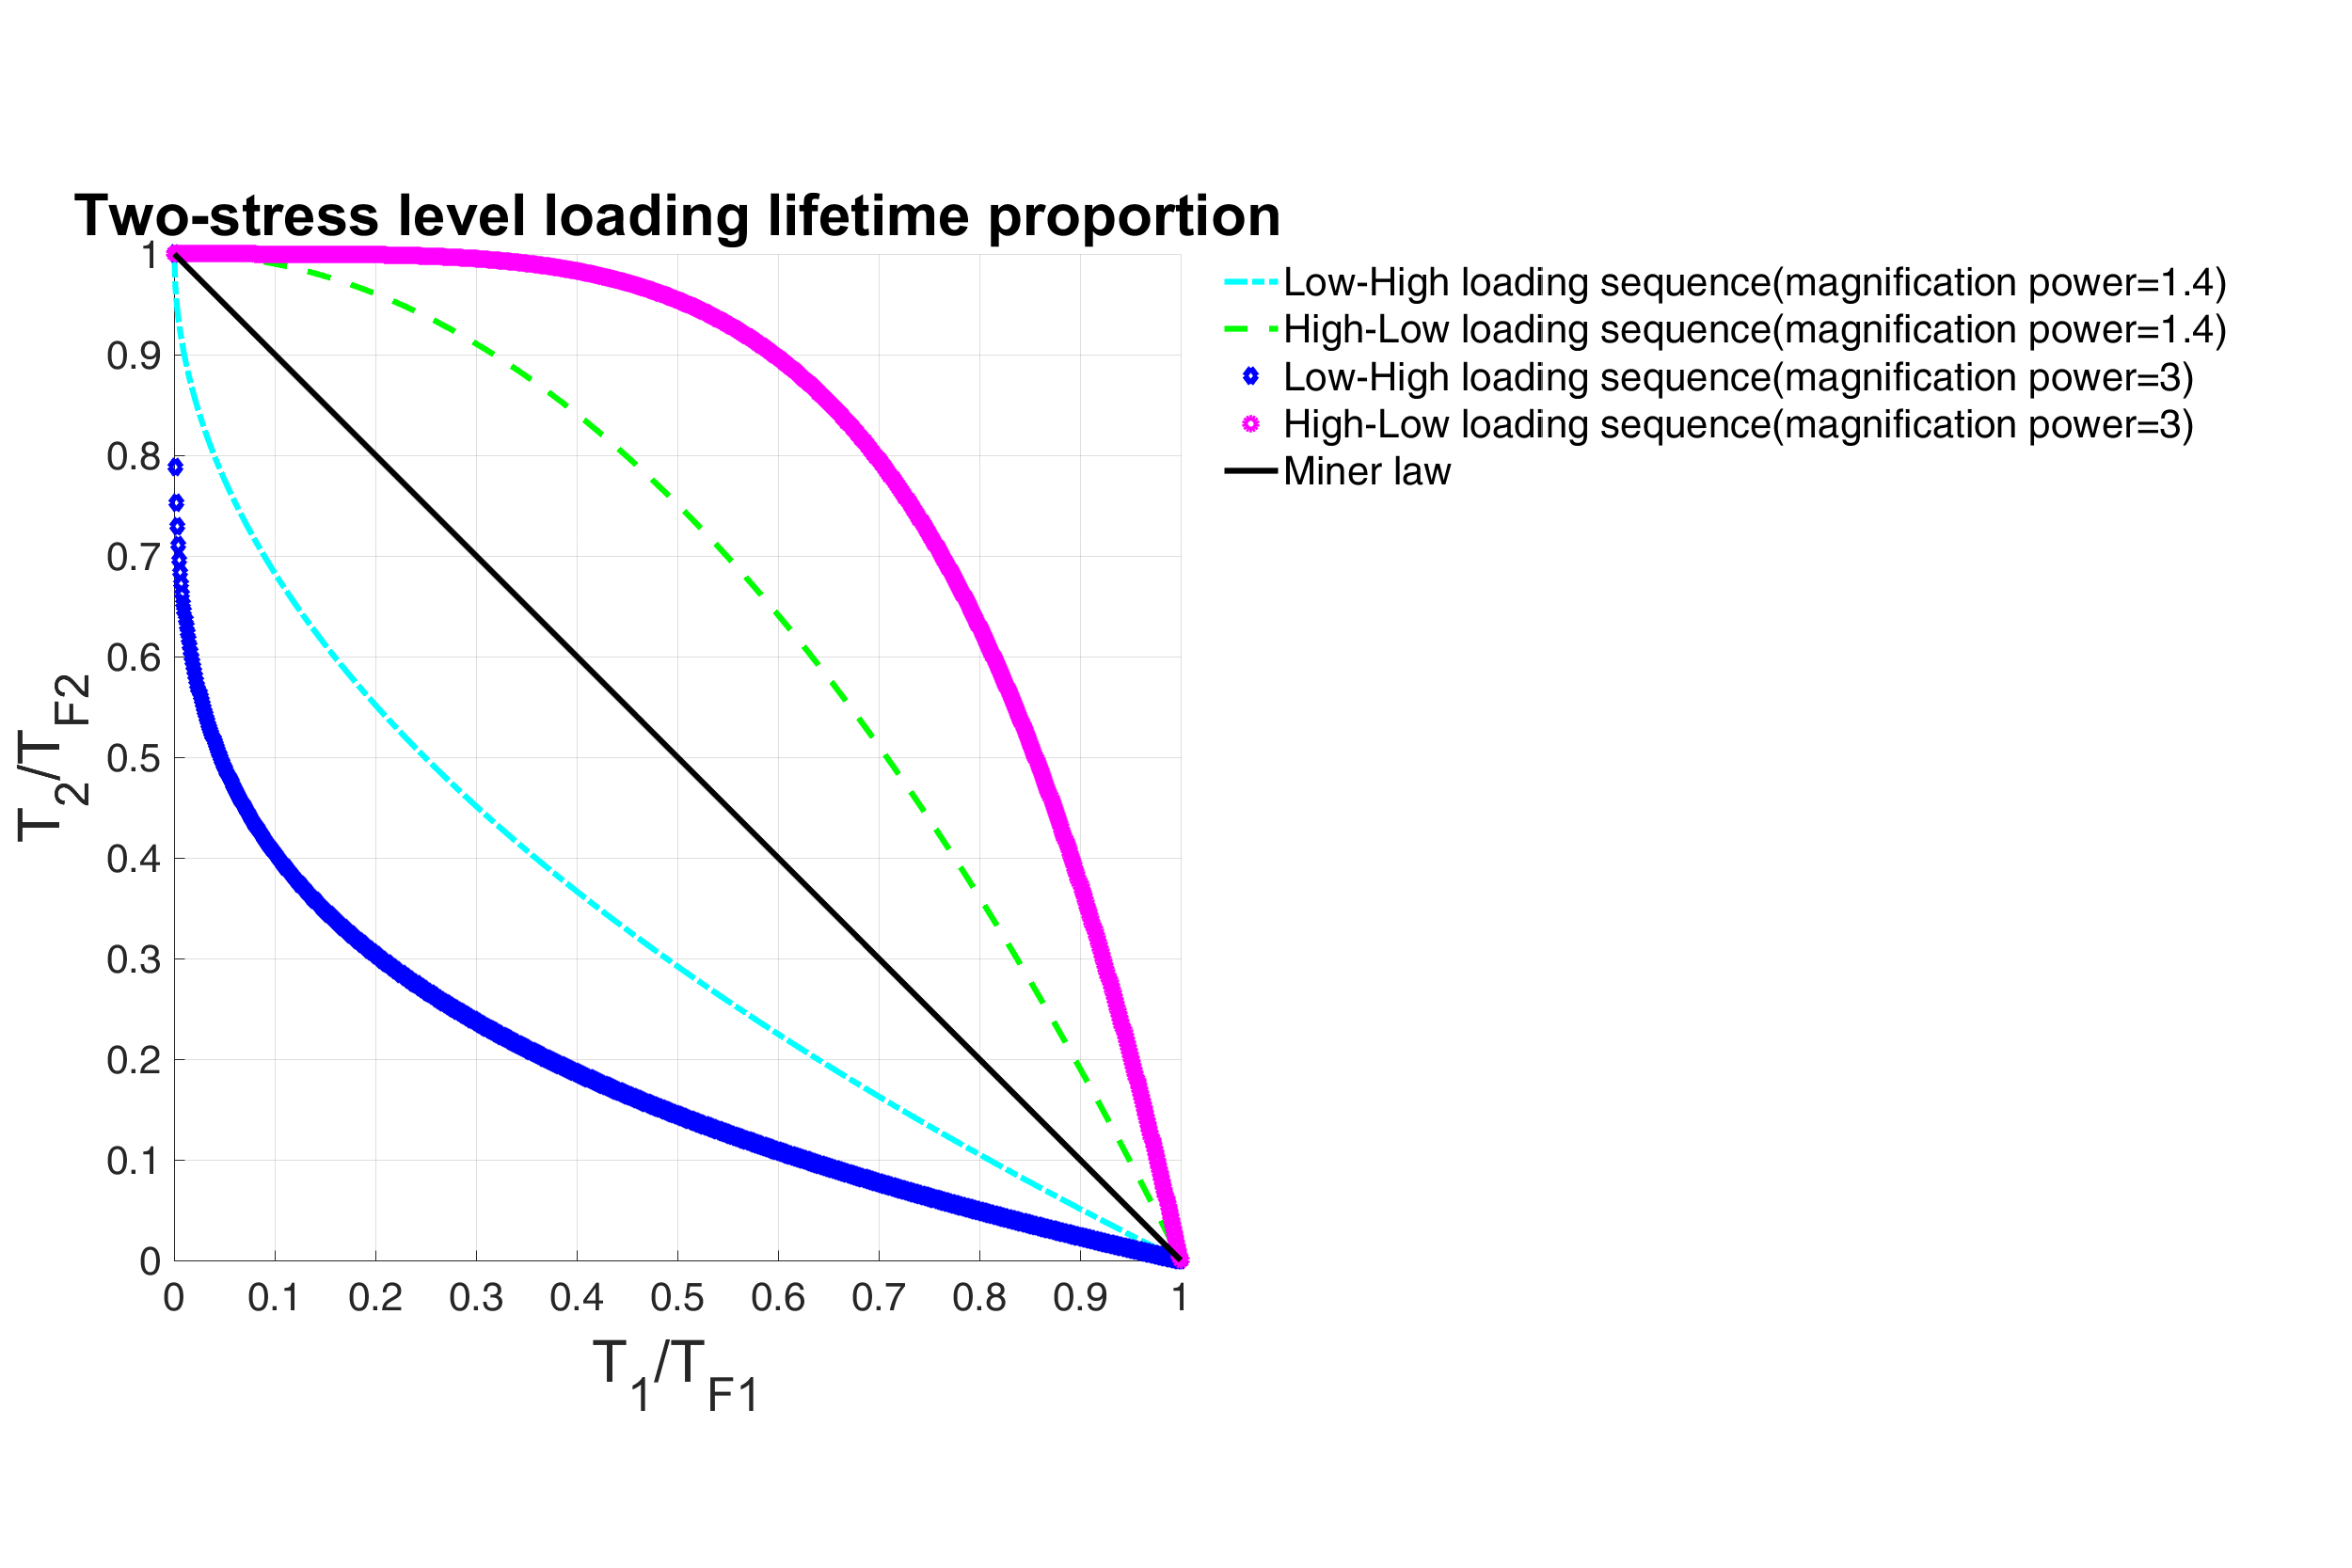
\includegraphics[width=\textwidth]{figures//sequence_ours.png} 
	\caption{Major damage effect using different $f(\beta)$ on sequence effect figure}
	\label{fig.sequenceours}
\end{figure}
$$f(\beta)=\beta-0.1.$$

 We can find that the numerical results are satisfactory with magnification factor $f(\beta)$, the dispersion figure with distinction of major damage is depicted in \figref{fig.Cetimerr}. Here it is necessary to control the parameter $a$ to make sure $\alpha>0$ in the most severe situation.

\begin{figure}[!h]
	\centering
	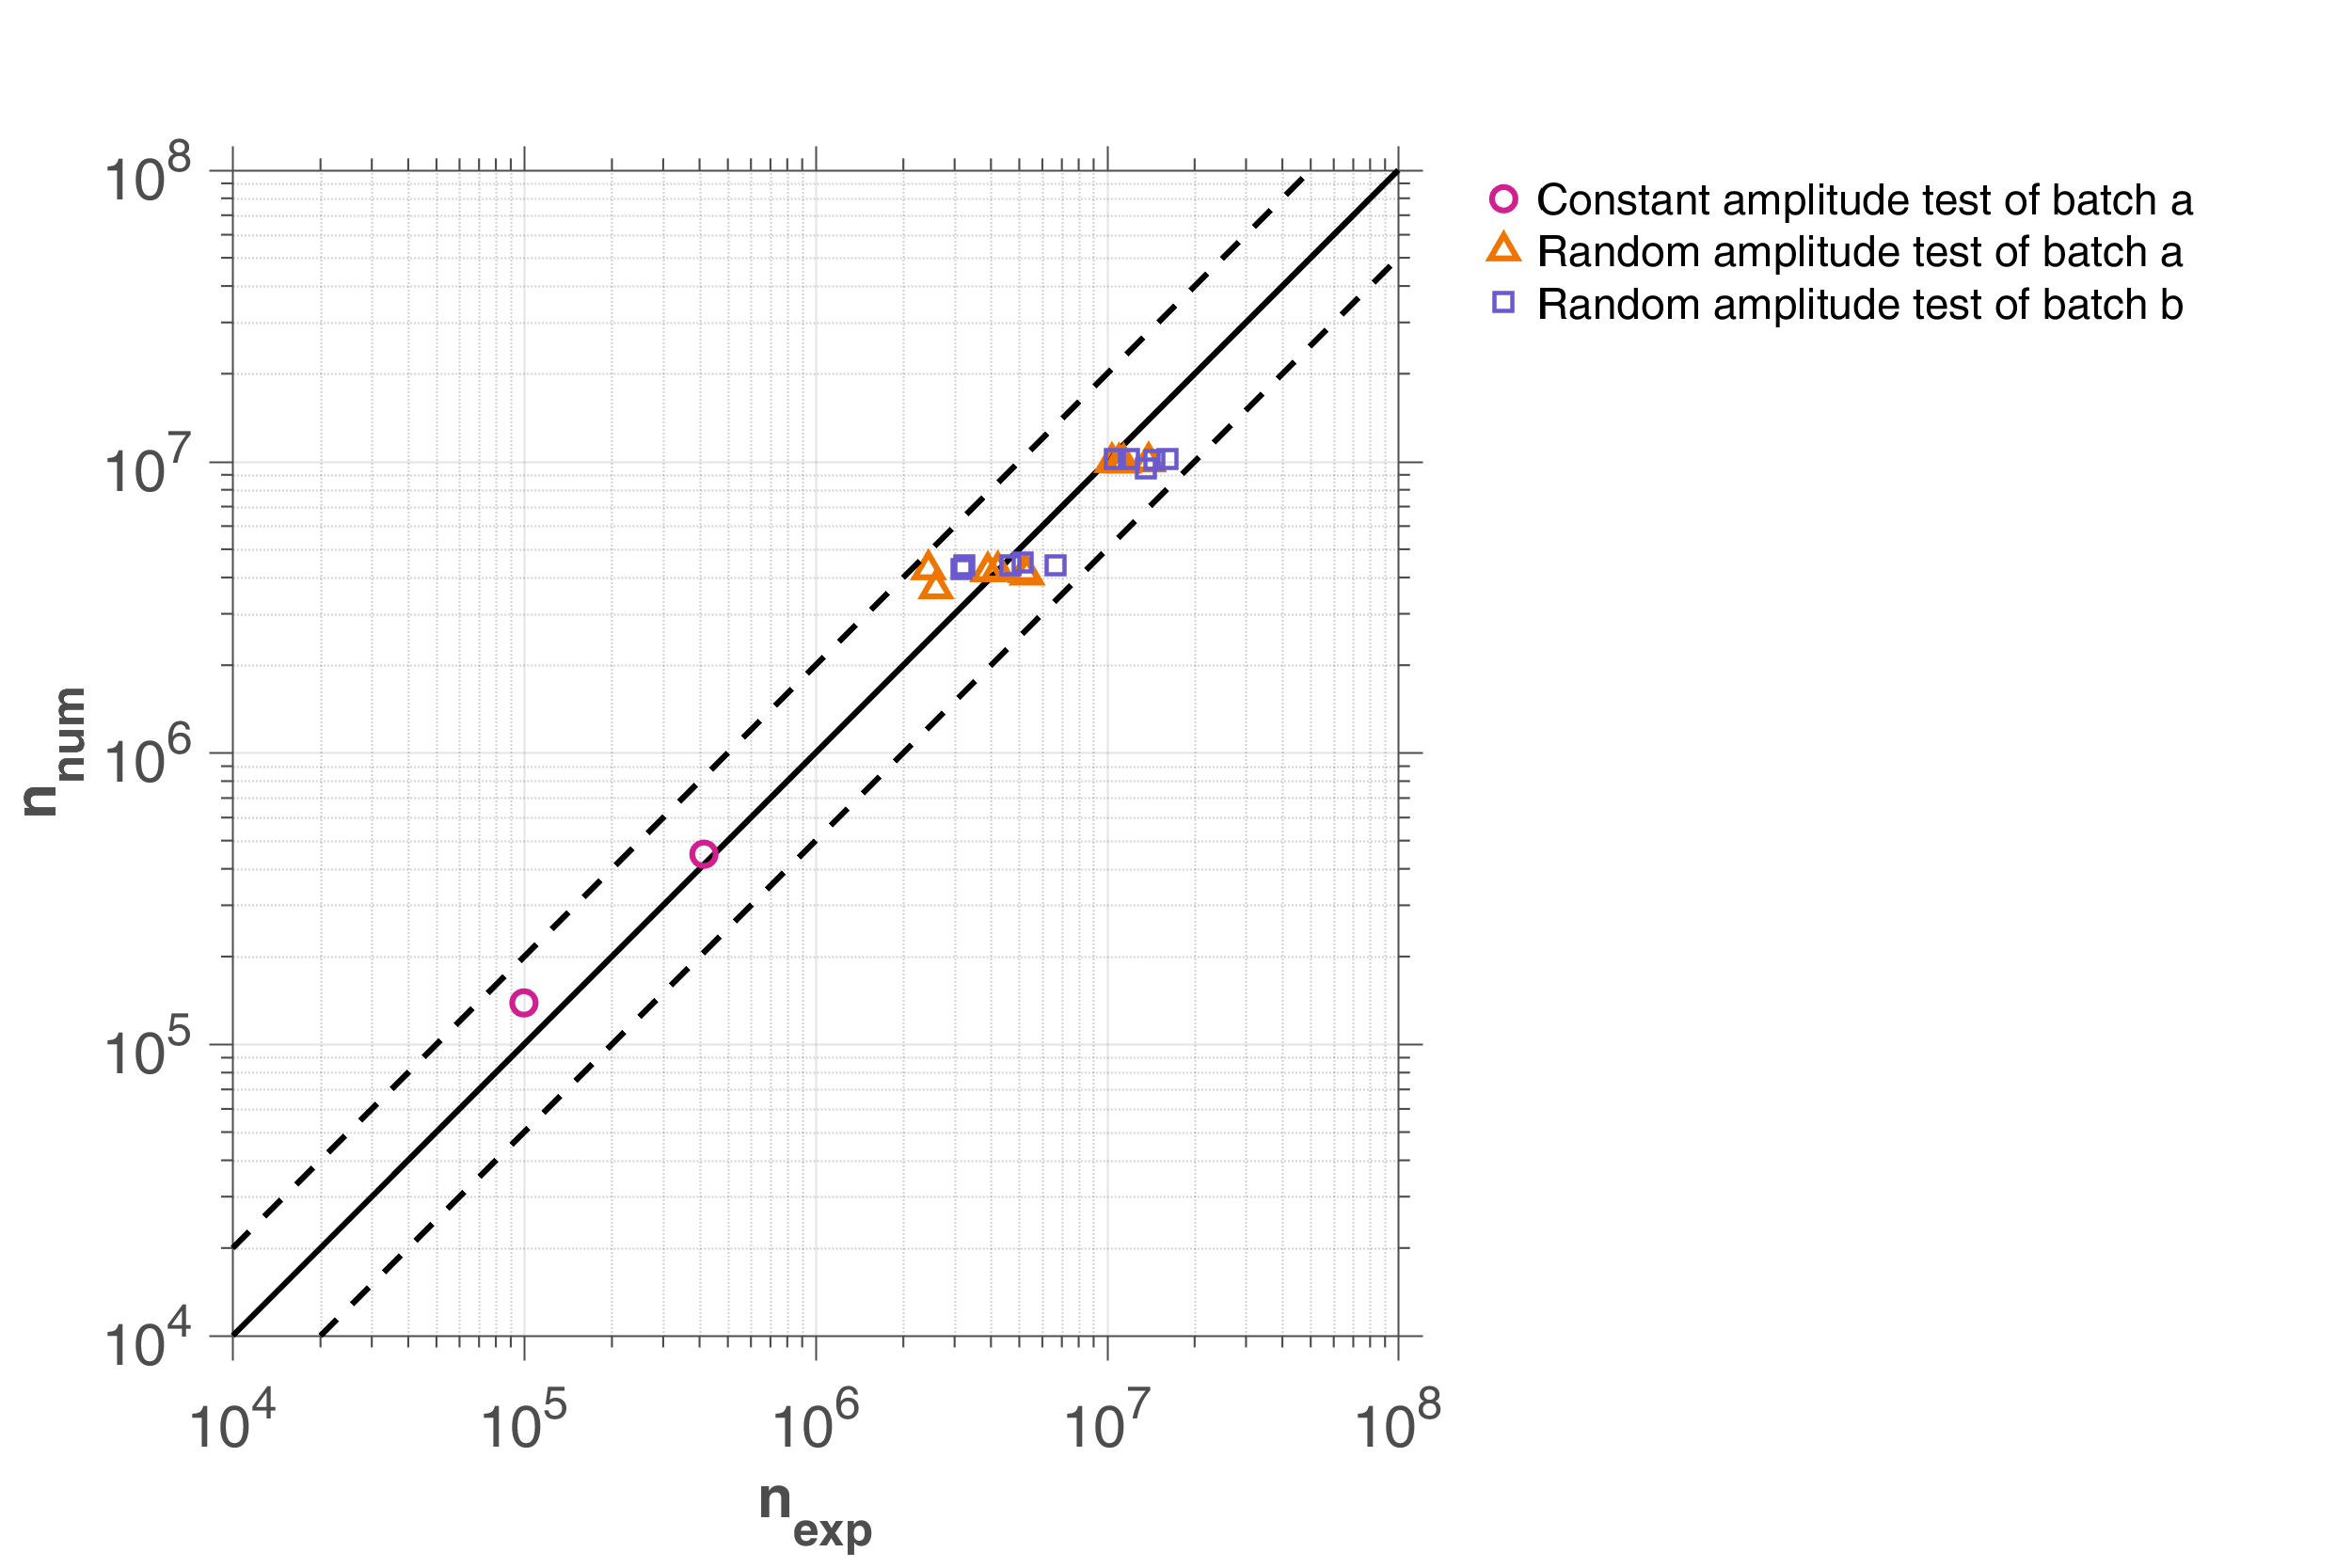
\includegraphics[width=\textwidth]{figures//Cetim_err.png} 
	\caption{Comparison between experimental and numerical results of 1D cyclic and random loading on aluminum fatigue tests by Cetim}
	\label{fig.Cetimerr}
\end{figure}


\subsection{Tests on ER7(clement roux thesis without $\sigma_{-1}$)}
This part is for the goal of complete the fatigue data in order to choose a method to calculate the fatigue life adapted to our situation(multiaxial stress trajectory with out of phase load). The material constants are shown in Table.\ref{tab:ER7}.
\begin{table}[!h]
	\centering
	\begin{tabular}{ll}
		\hline
		\textbf{Parameters}                                       & \textbf{Value}                    \\ \hline
		Young's modulus                                          & $E=214$ GPa                       \\
		Macroscopic yield stress                              & $\sigma_y=405$ MPa              \\
		Ultimate stress                  & $\sigma_u=720$ MPa                        \\ \hline
	\end{tabular}
	\caption{Material parameters}
	\label{tab:ER7}
\end{table}

\subsection{Tests on Aluminum 6082T6(habibou paper without specific data)}
Experimental results obtained by Susmel and Petrone [?] are
used to validate the method. Experimental tests were made on
plain specimens of Aluminum 6082T6. The loadings considered
are fully reversed bending, fully reversed torsion, bending and torsion in-phase, and bending and torsion out-of-phase with a phase
difference of 90$^\circ$.

\begin{comment}
\newpage
\subsection{1D data from PSA}
In this test, we reconstruct a unidimensional macroscopic stress history from recorded force data proposed by PSA group. 
\begin{figure}[!h]
	\centering
	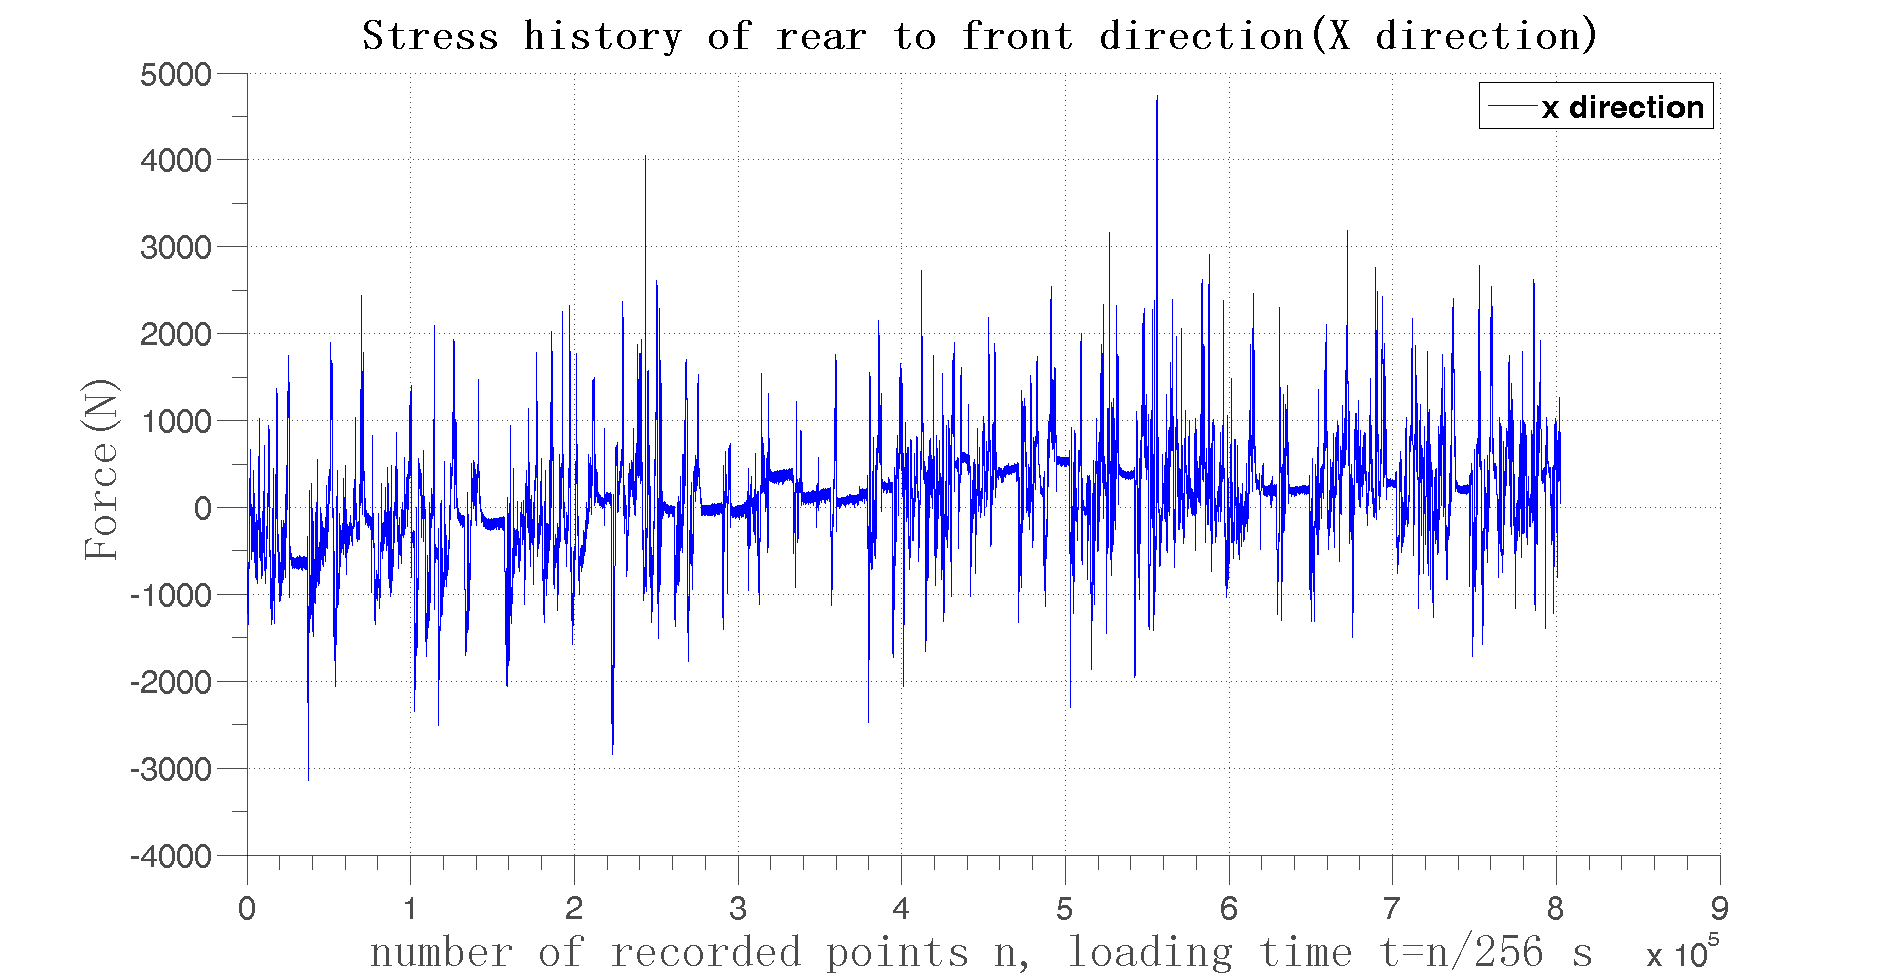
\includegraphics[width=\textwidth]{figures//x.png} 
	\caption{Loading history of X direction, force vs the record index n, with 256 sample recorded per second}
	\label{x}
\end{figure}

The force on wheel is firstly considered as under uniaxial loading $F_x$. Here we temporally set $\Sigma_x=F_x/A$ where $A=\dfrac{1}{1e6} m^2$ is the area of force, and $W_0=3e6 J$. The other data are as Table.\ref{Sin}. The plot of $\left\|  \uline{\uline{S}}-\uline{\uline{b}}\right\|_{trial}$ and $\left\|  \uline{\uline{S}}-\uline{\uline{b}}\right\|$ at 2 different scales are shown in \figref{trialreal}. The damage evolves like \figref{damage1d}. 

\begin{figure}[!h]
	\centering
	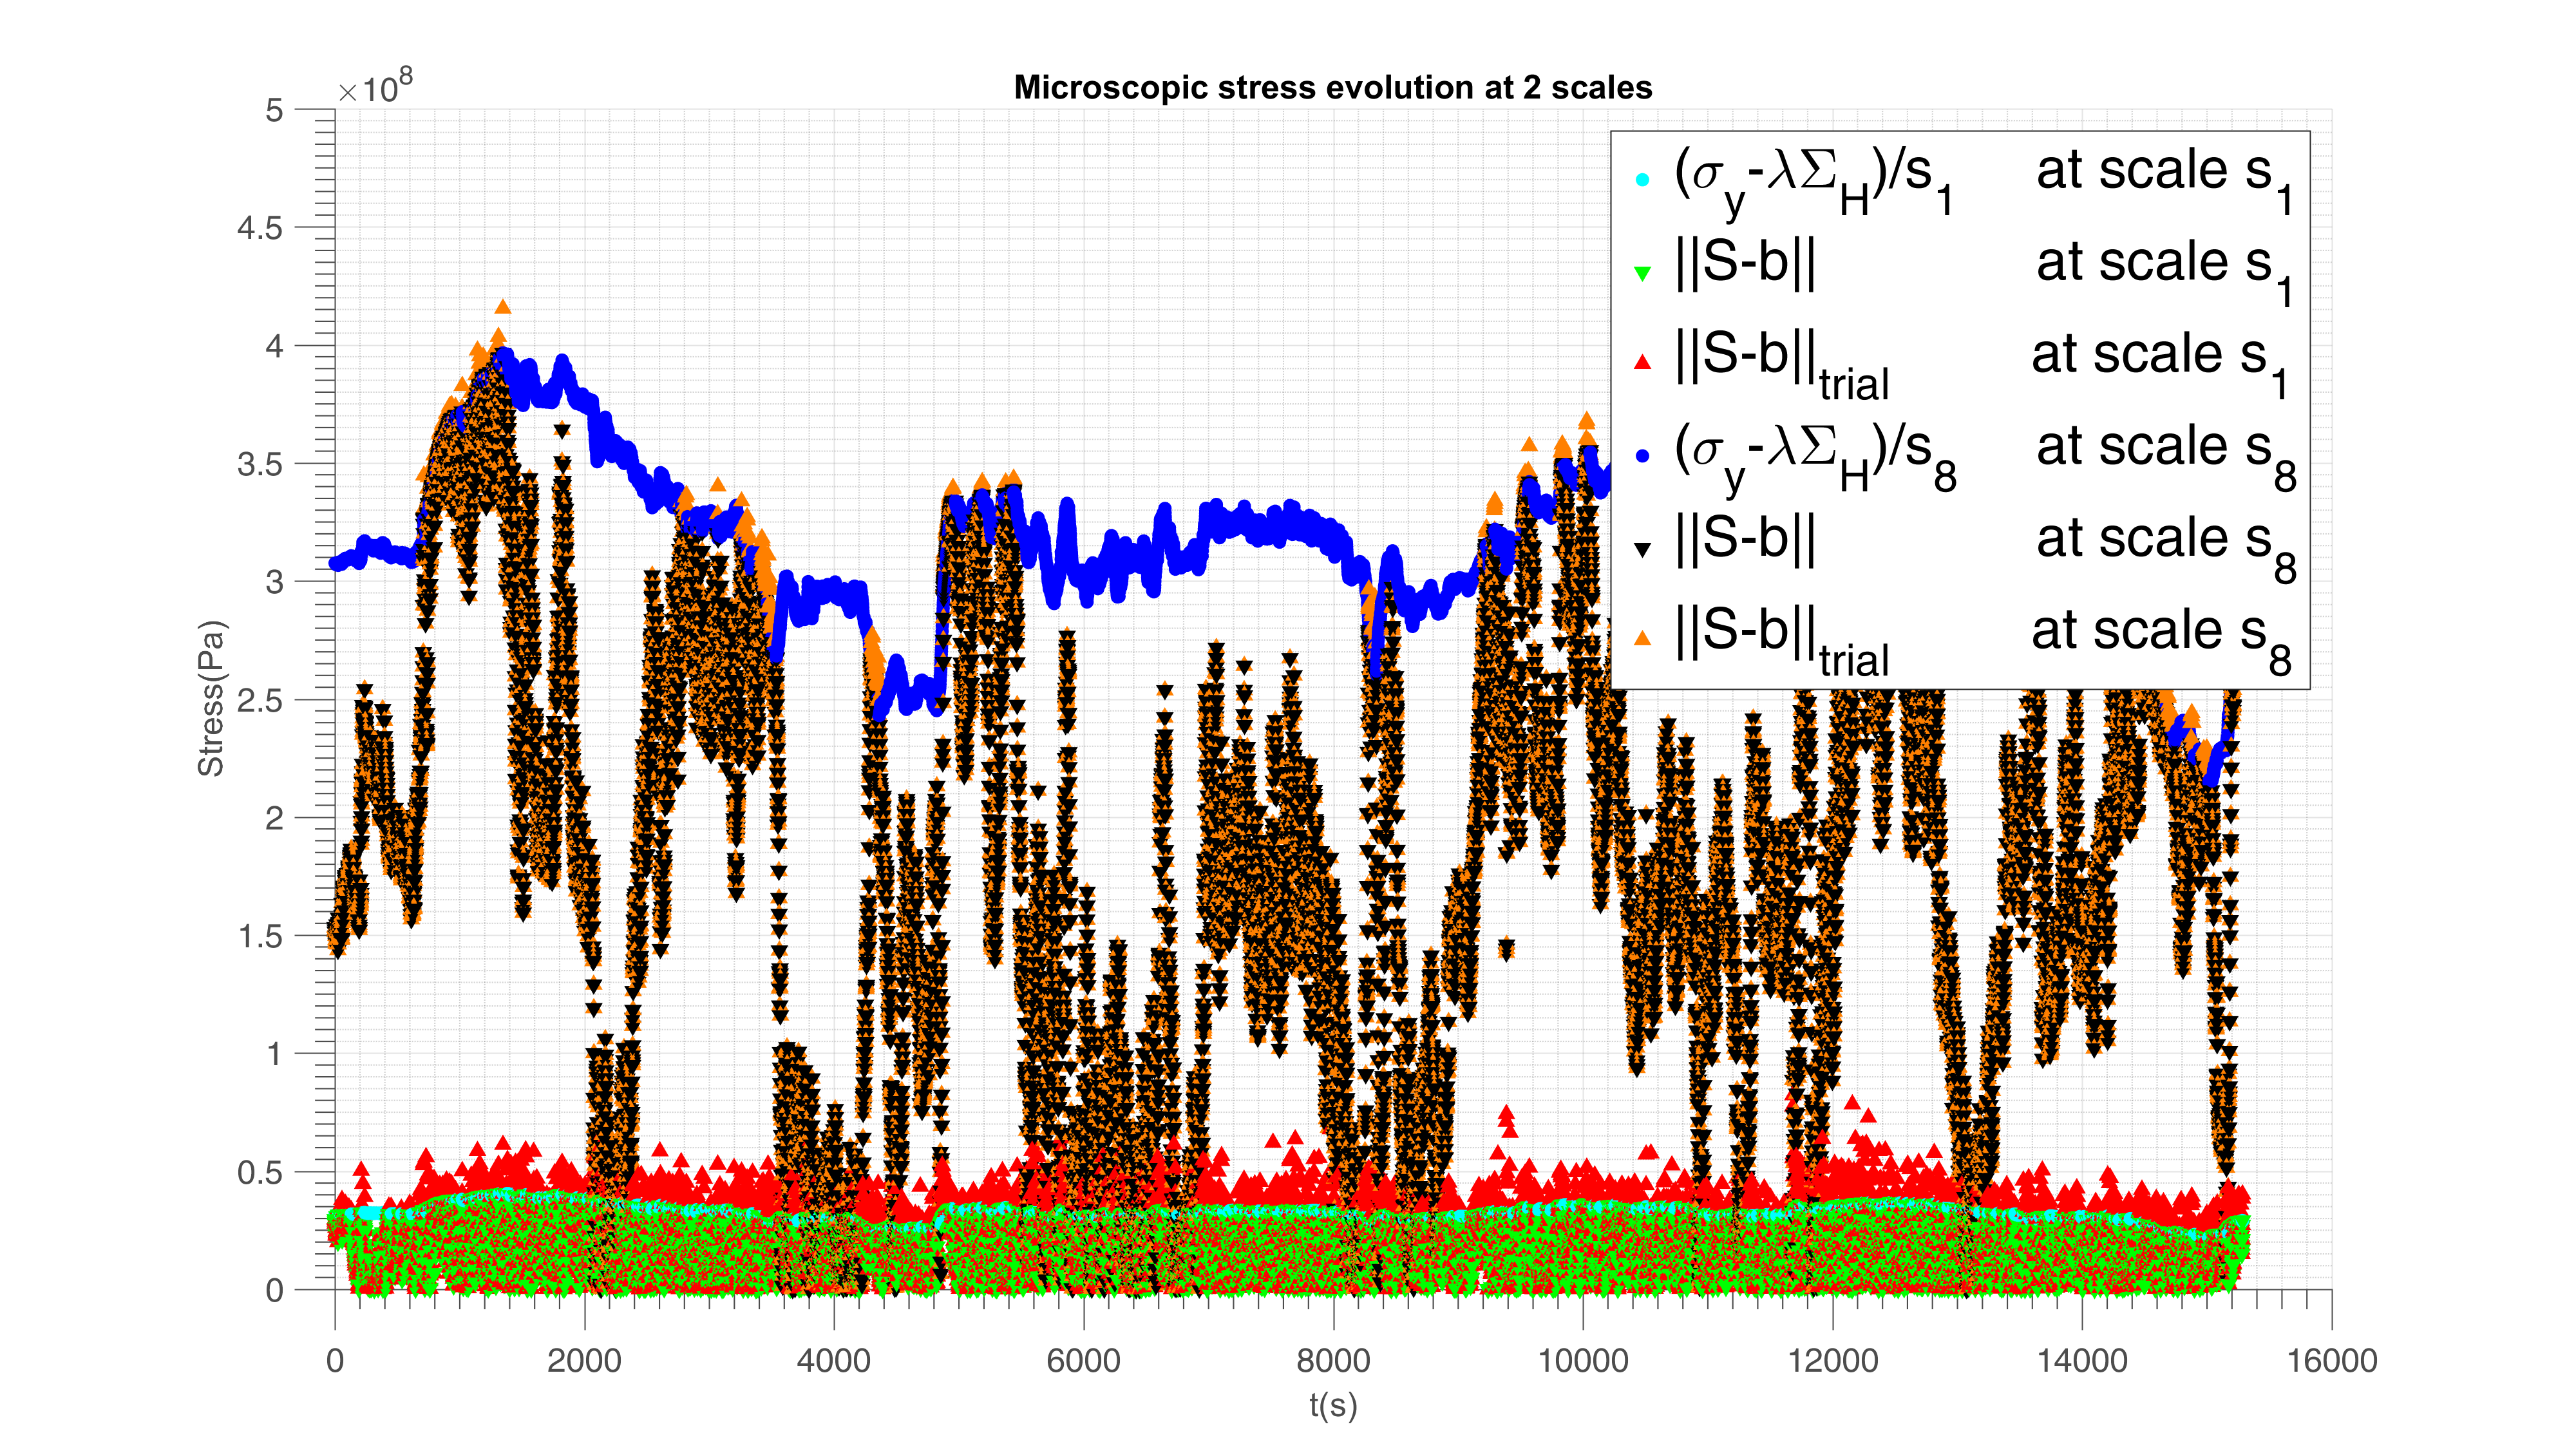
\includegraphics[width=\textwidth]{figures//trialreal1d1.png} 
	\caption{$\left\|  \uline{\uline{S}}-\uline{\uline{b}}\right\|_{trial}$ and $\left\|  \uline{\uline{S}}-\uline{\uline{b}}\right\|$ evolution with time under different weakening scales in PSA load history}
	\label{trialreal}
\end{figure}
\begin{figure}[!h]
	\centering
	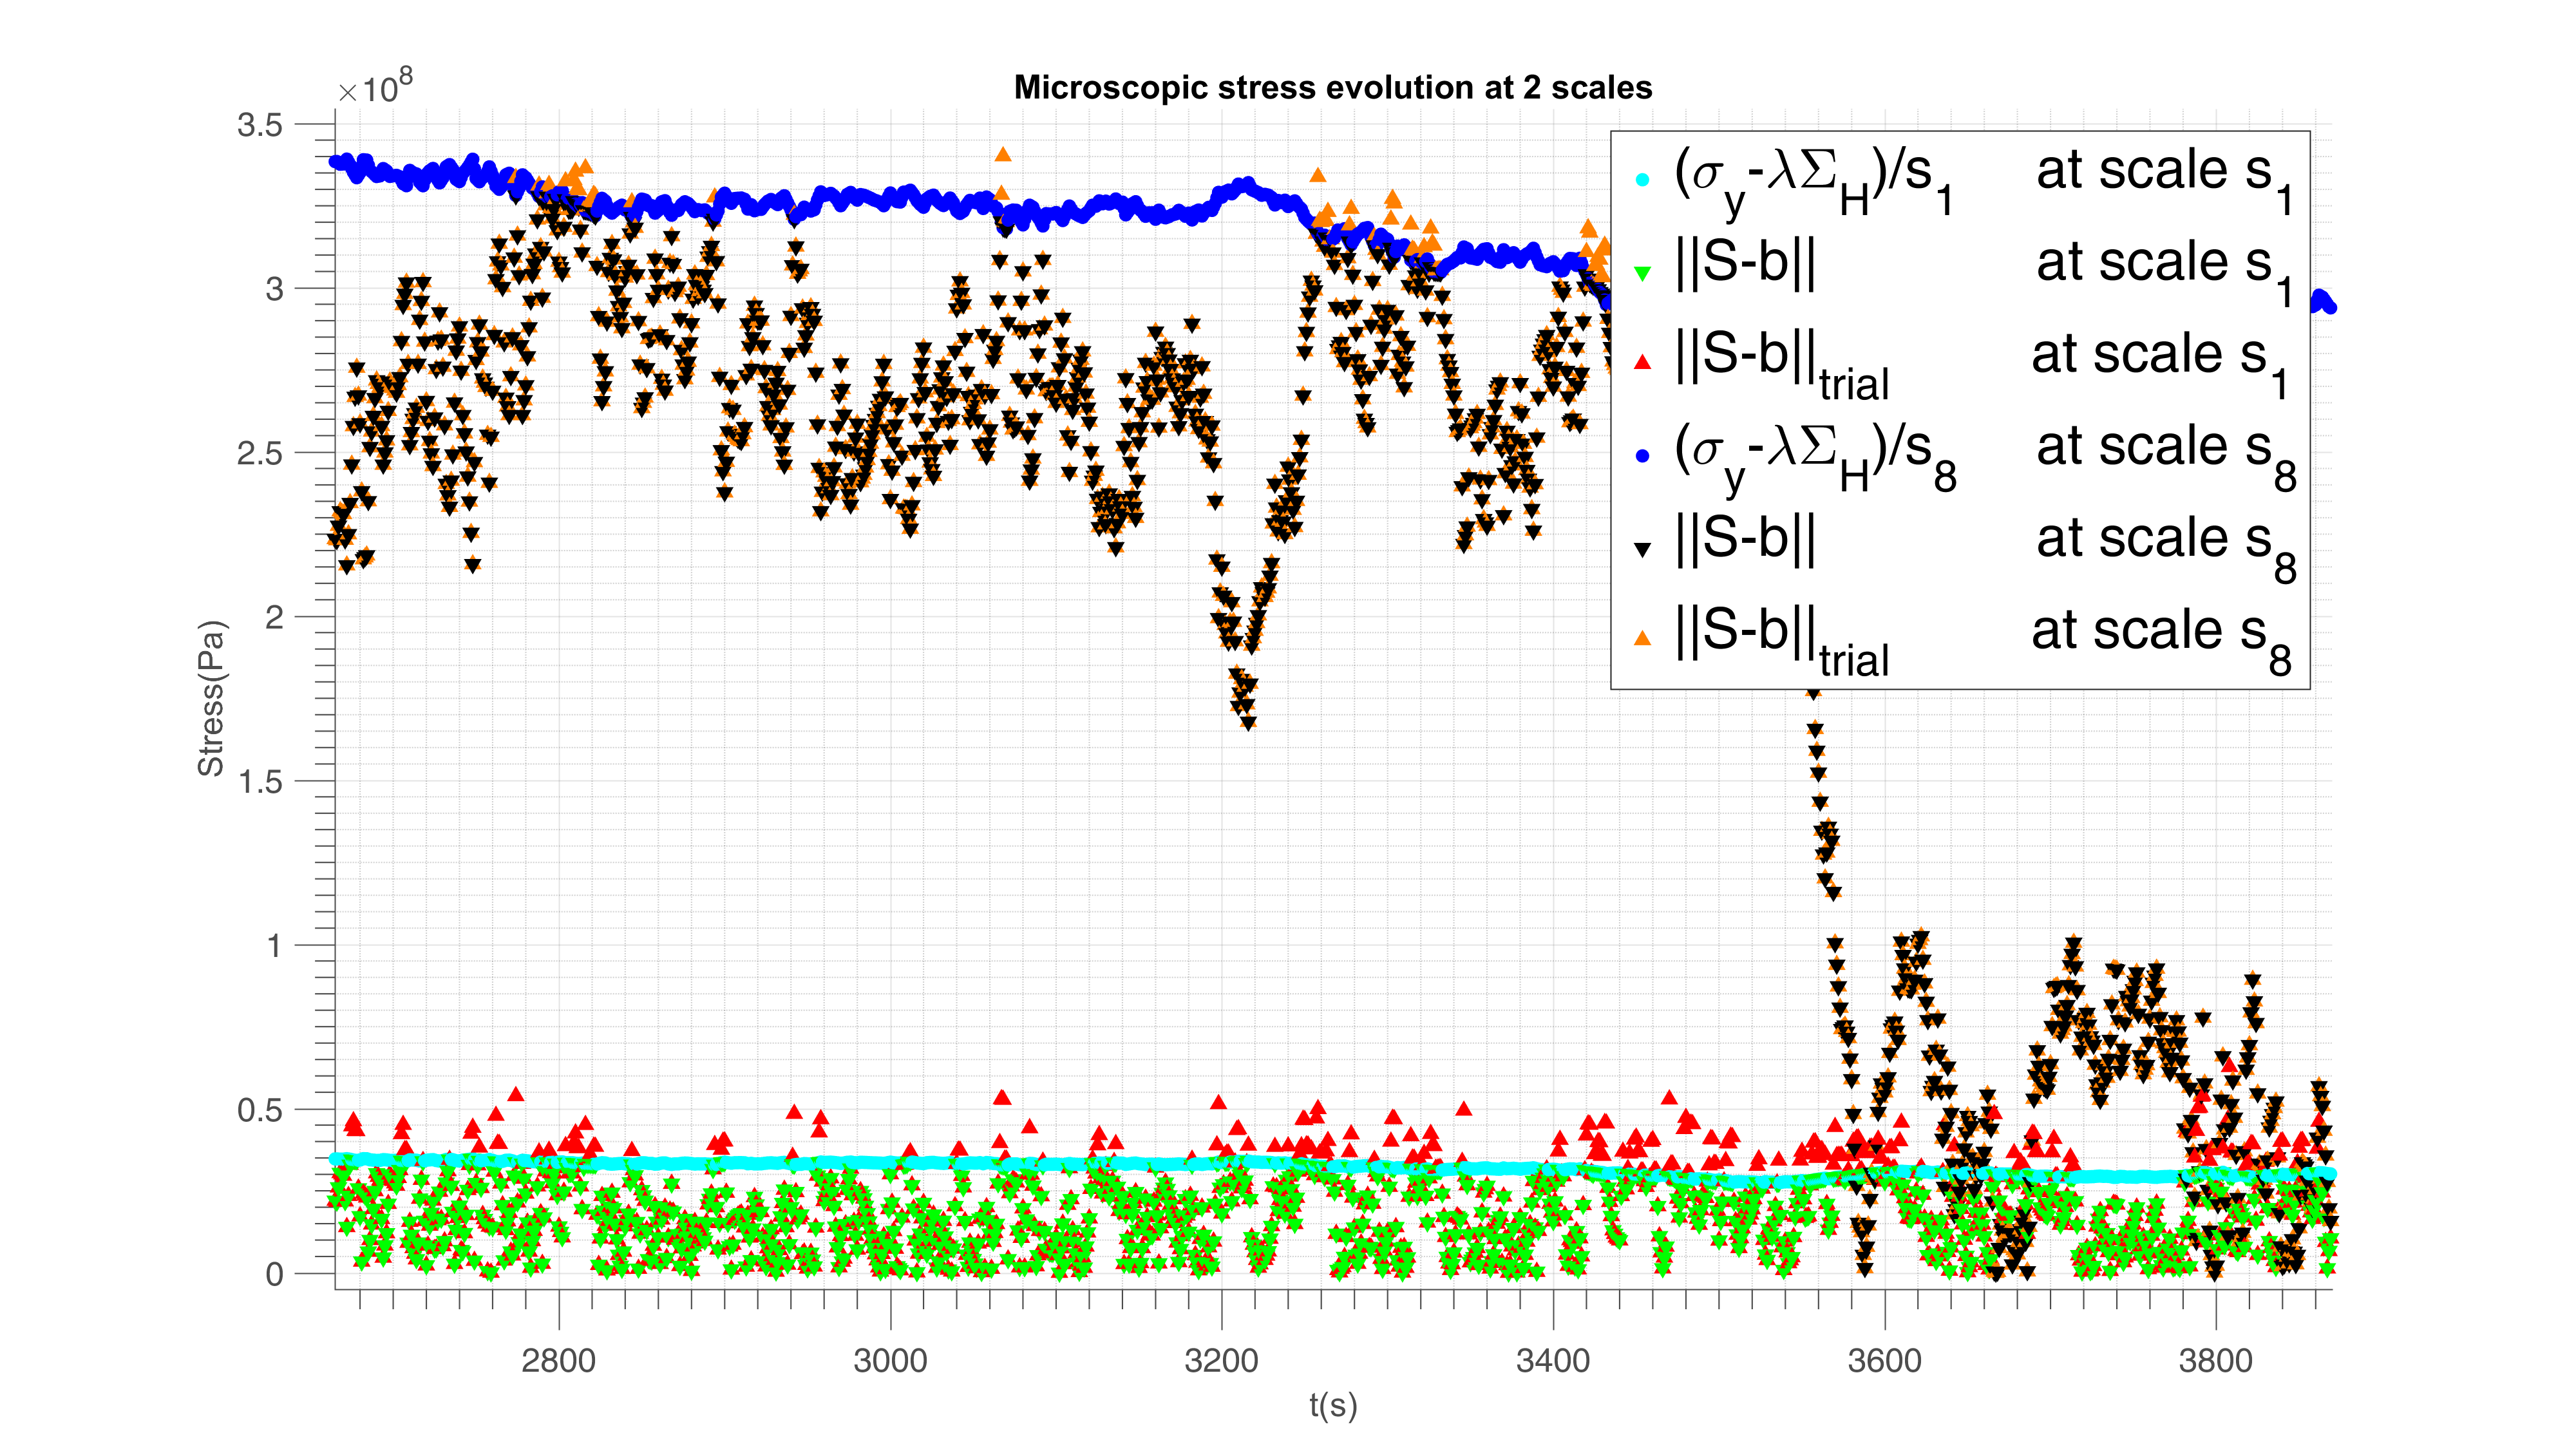
\includegraphics[width=\textwidth]{figures//trialreal1d2.png} 
	\caption{Circled area magnification in \figref{trialreal} where there is more $\left\|  \uline{\uline{S}}-\uline{\uline{b}}\right\|_{trial}>\left(\sigma_y-\lambda \Sigma_H\right)$(plasticity)  at $s_1$ than at $s_8$}
	\label{trialreal1d2}
\end{figure}
\begin{figure}[!h]
	\centering
	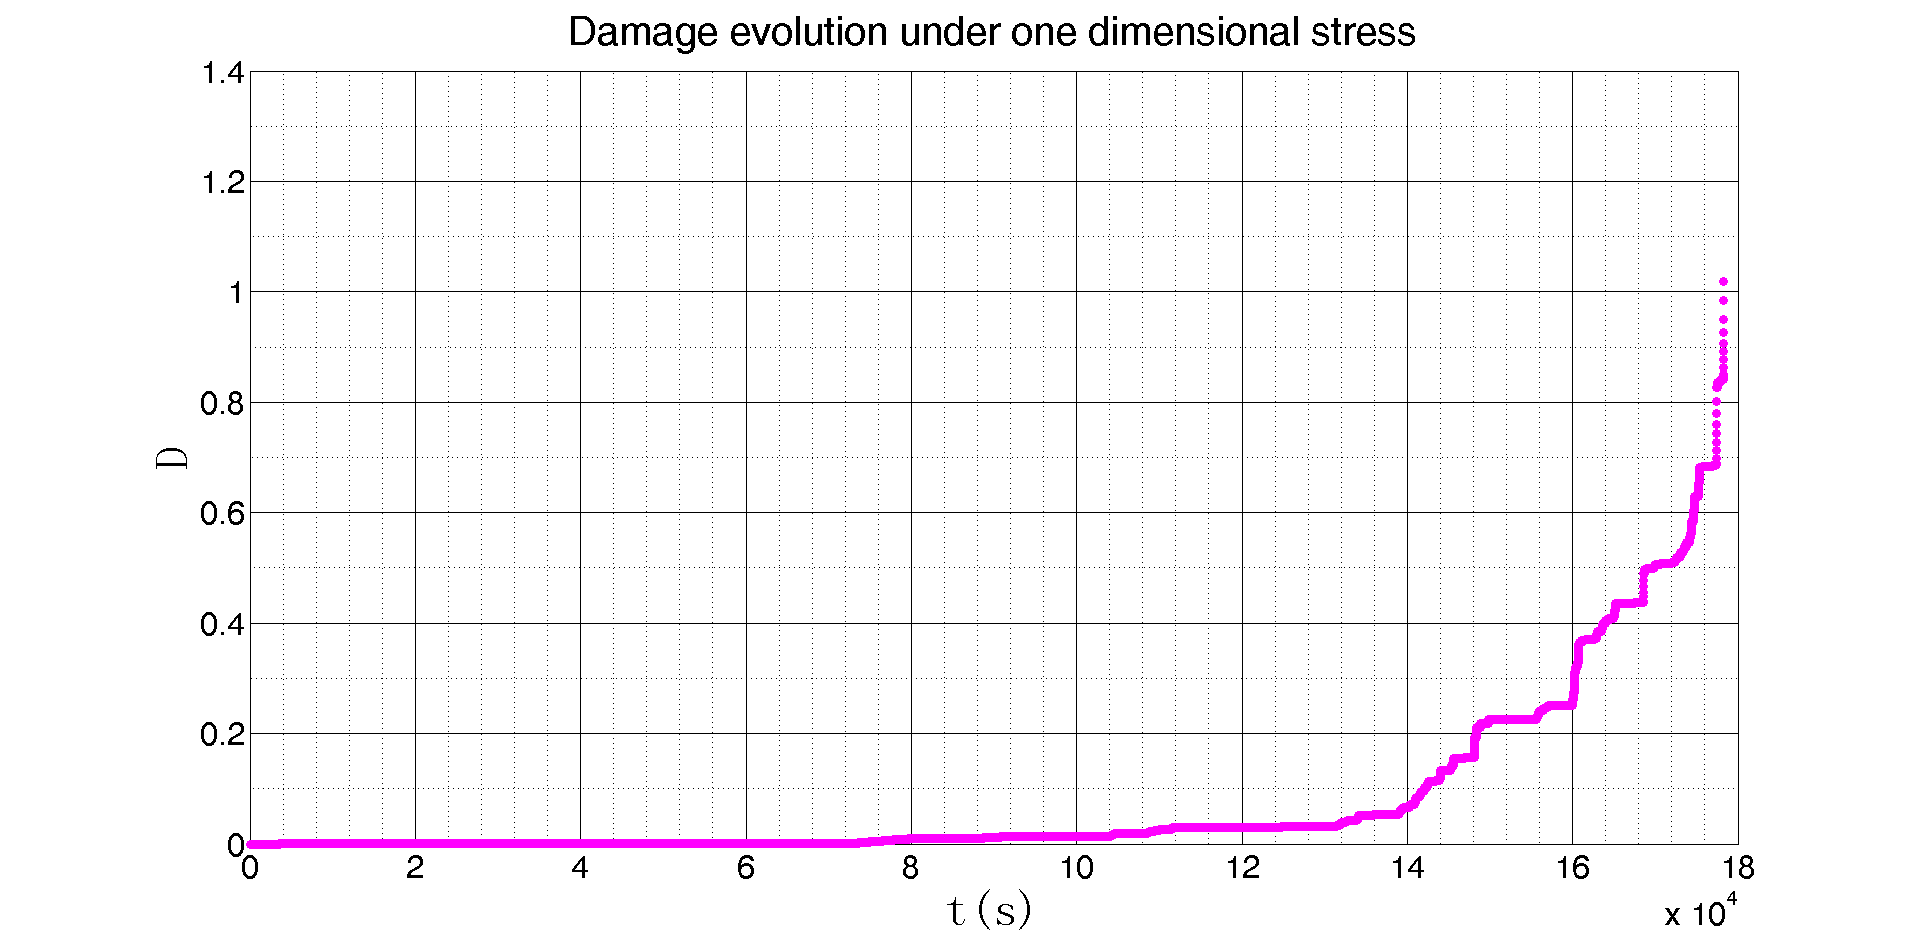
\includegraphics[width=\textwidth]{figures//damage1d.png} 
	\caption{Damage evolution with time at one dimension PSA load history}
	\label{damage1d}
\end{figure}

 \newpage
 \subsection{Multi-dimensional application to PSA data}
 We now consider a situation where we have force recorded measured in 3 different directions as shown in \figref{xyz}.
 \begin{figure}[!h]
 	\centering
 	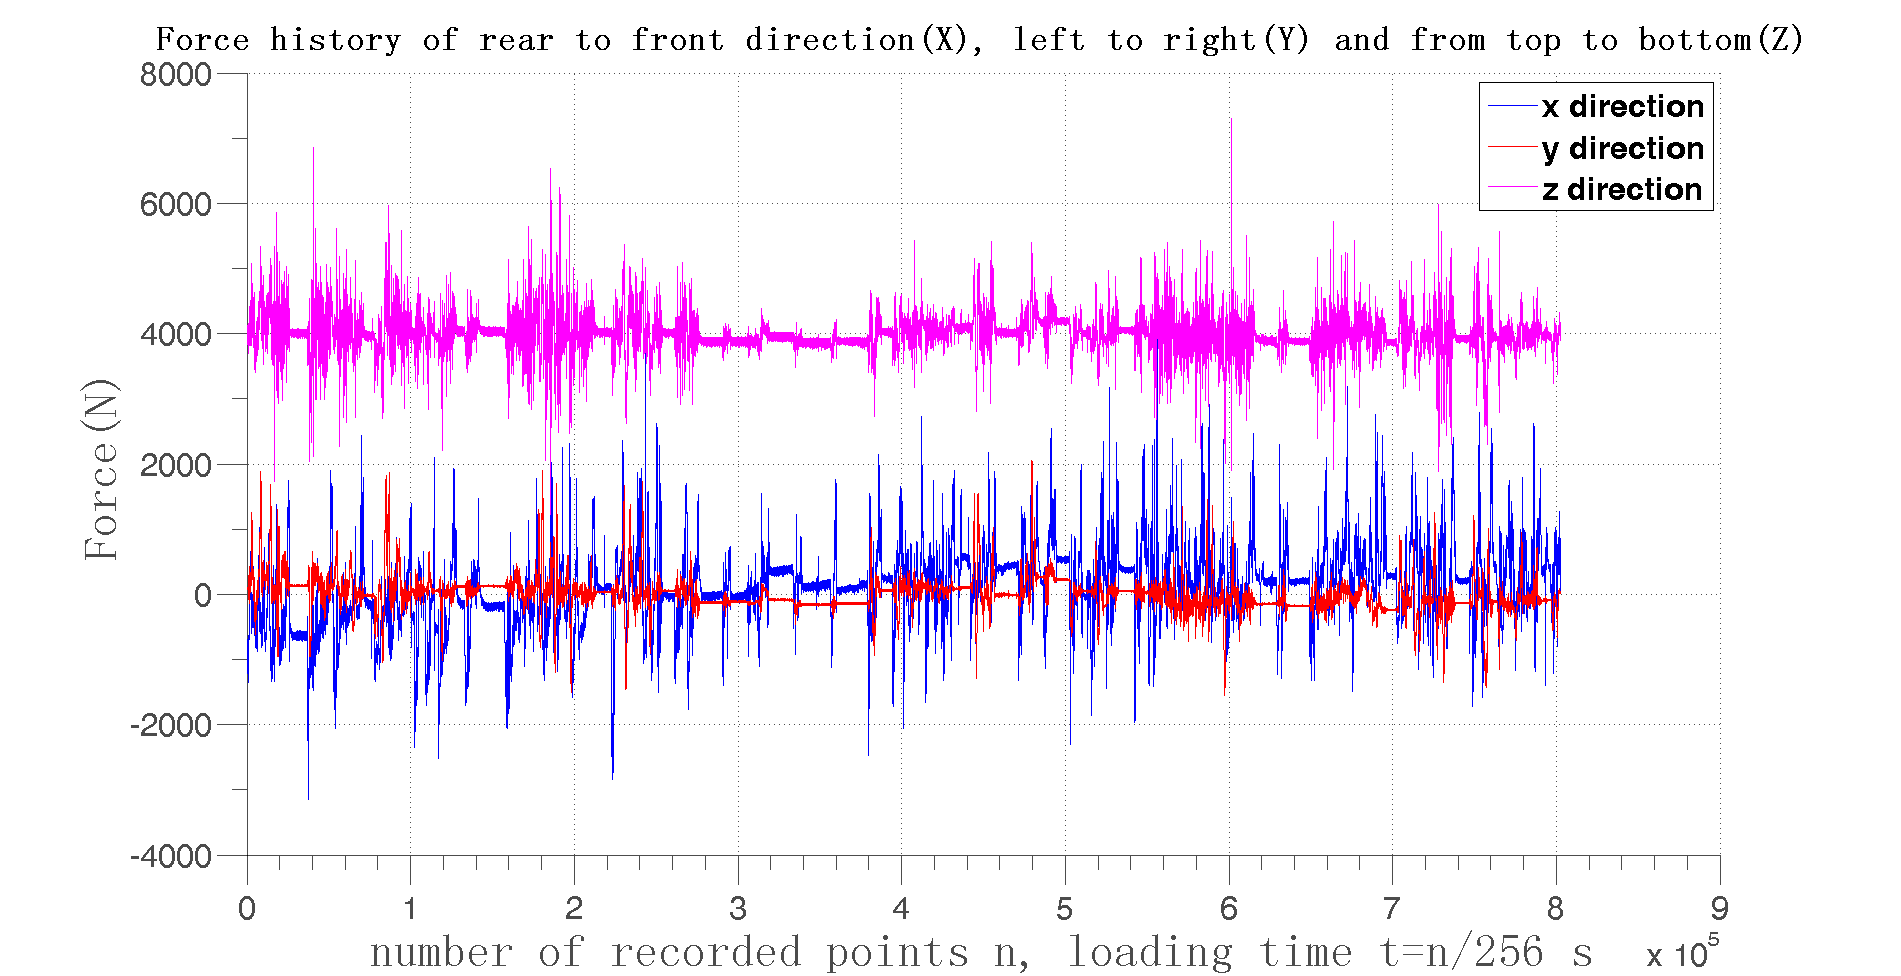
\includegraphics[width=\textwidth]{figures//xyz.png} 
 	\caption{Loading history of 3 different directions}
 	\label{xyz}
 \end{figure}
  \begin{figure}[!h]
  	\centering
  	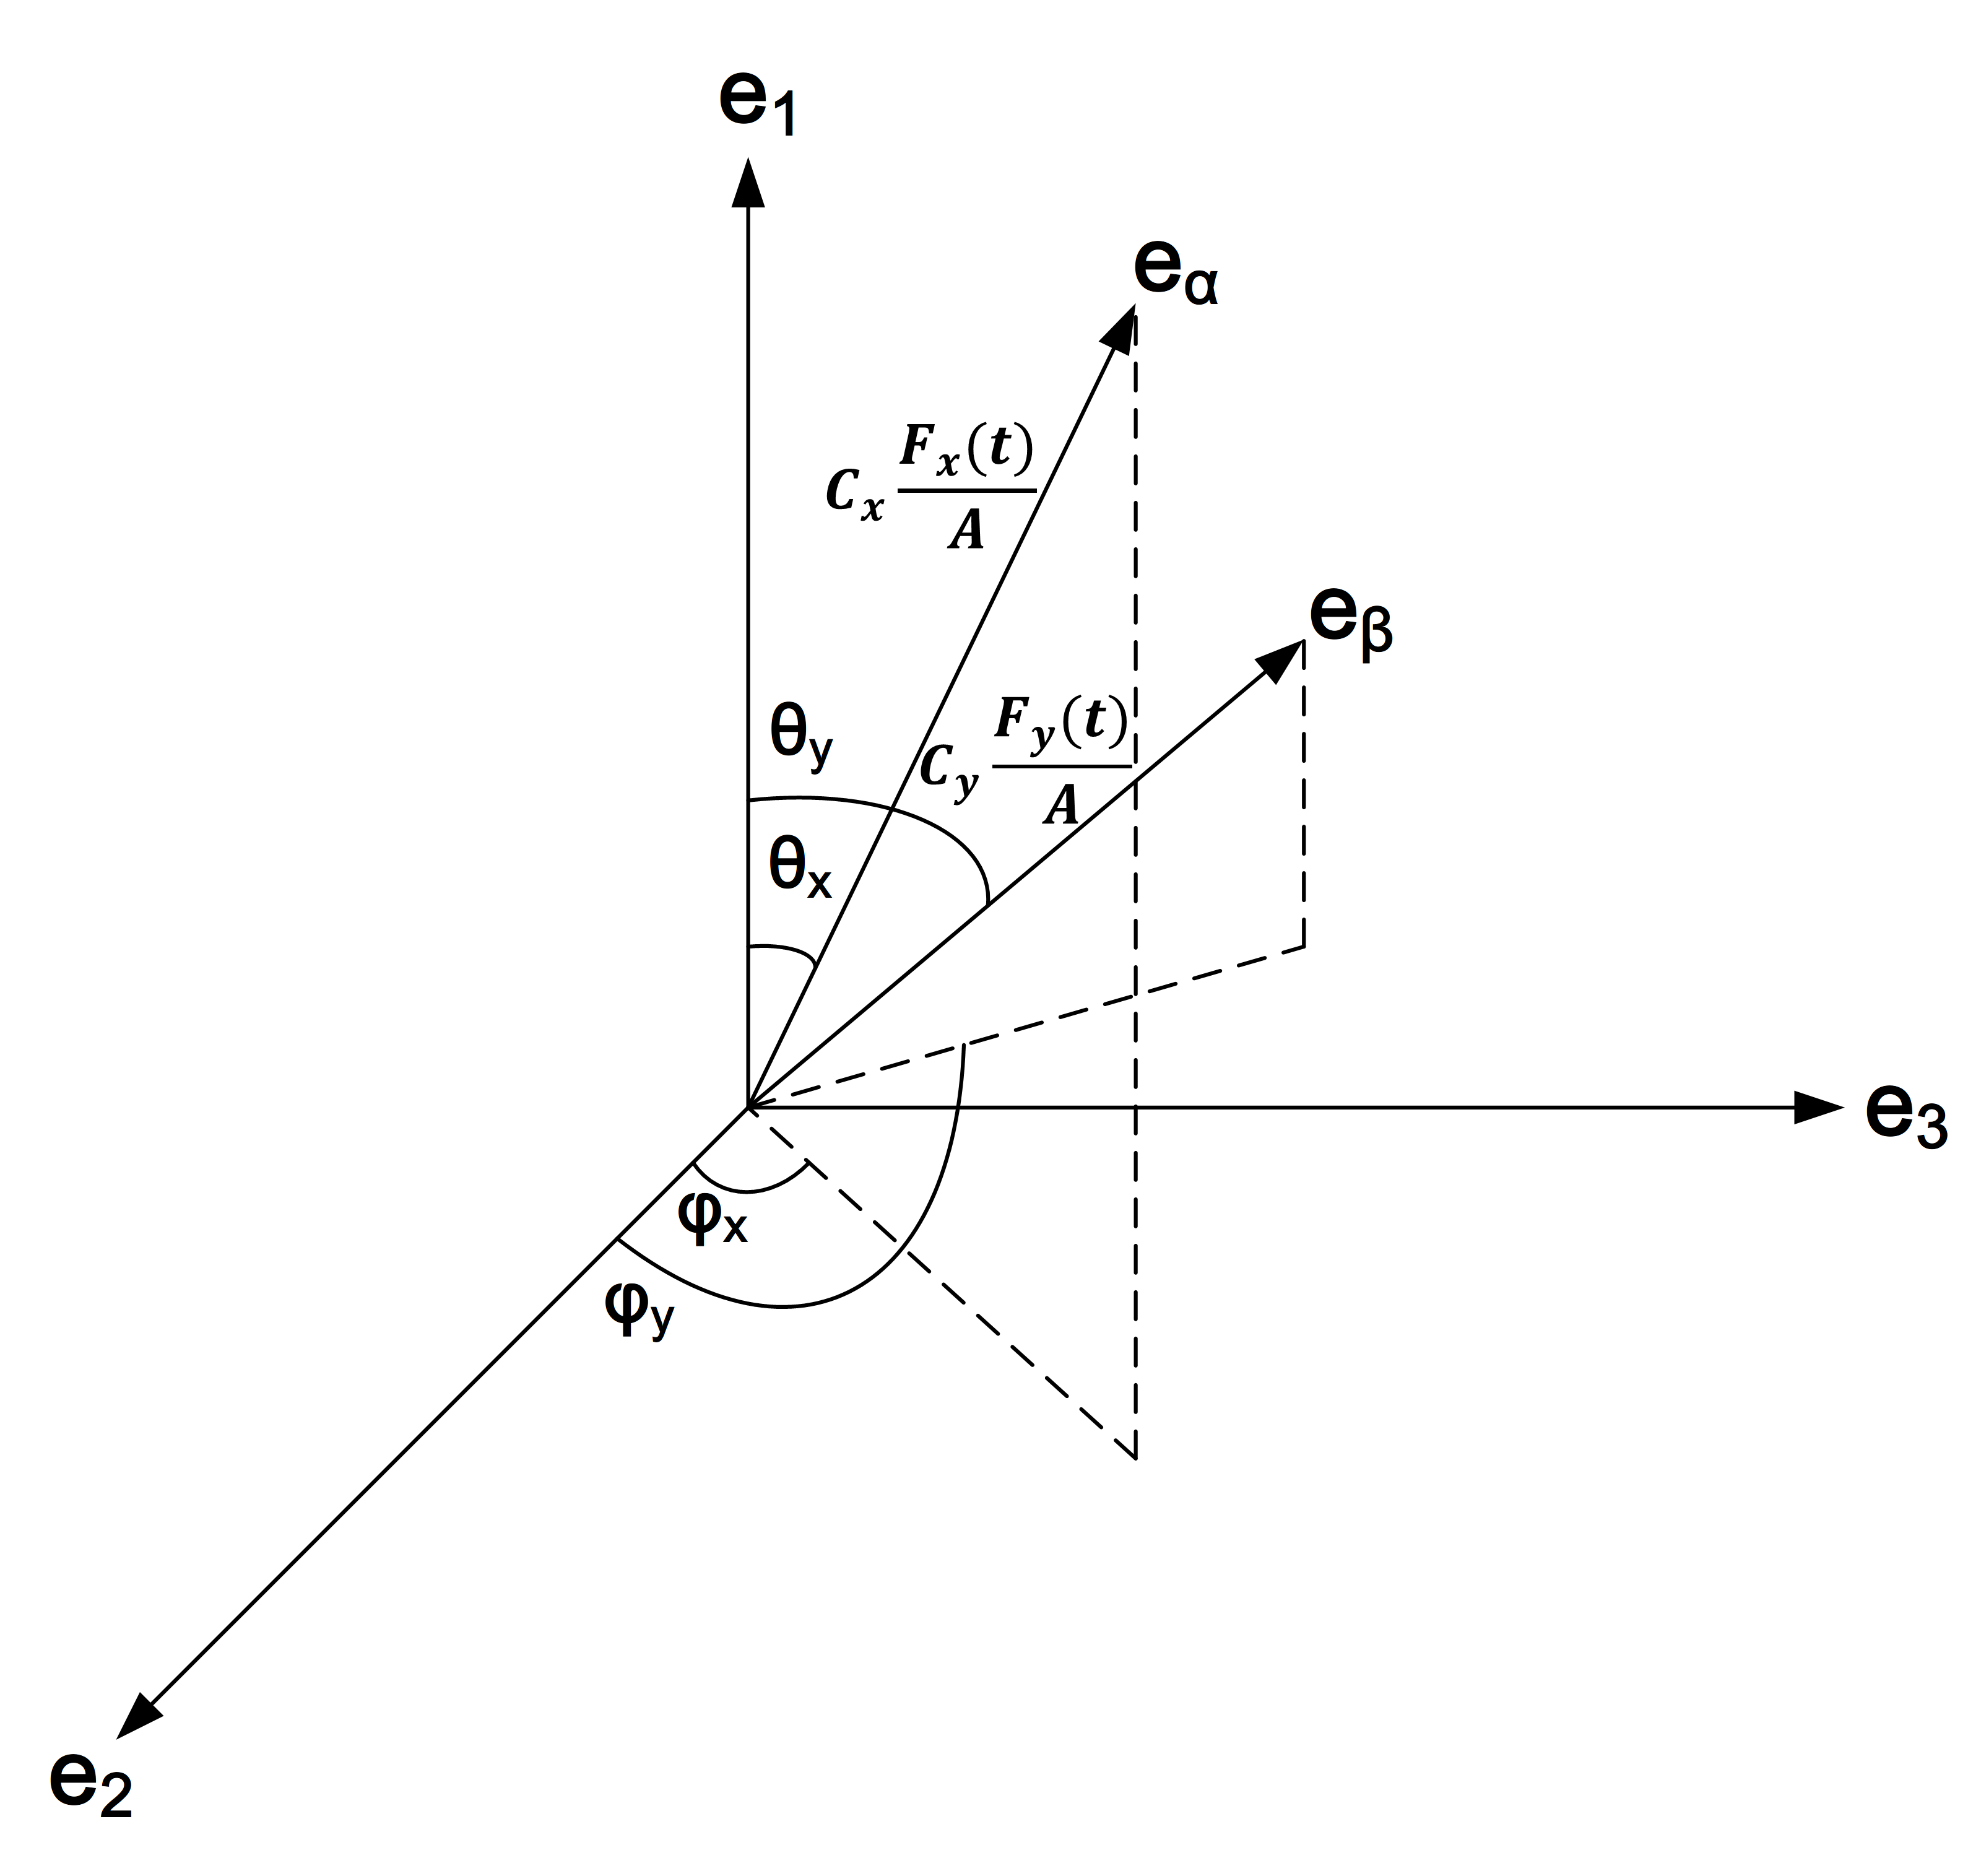
\includegraphics[width=0.7\textwidth]{figures//xab.png} 
  	\caption{Loading in 3 different directions}
  	\label{xab}
  \end{figure}
 In real case, the vertical force $F_z$ is much larger than the axial and horizontal forces $F_x$ and $F_y$, as shown in \figref{xyz}. However, in order to investigate large domains of interest, we first scale the axial and horizontal forces to reach comparable impact and transform them in principal stresses $c_x\dfrac{F_x}{A}$ applied along the stress principle vector $\uline{e}_\alpha$(respectively $\uline{e}_\beta$) that we choose randomly(\figref{xab}). We therefore consider the following macroscopic stress tensor:
 \begin{equation}
 \uline{\uline{\Sigma}}=\dfrac{F_z(t)}{A}\uline{e}_1\otimes \uline{e}_1+c_x\dfrac{F_x(t)}{A}\uline{e}_{\alpha}\otimes \uline{e}_{\alpha}+c_y\dfrac{F_y(t)}{A}\uline{e}_{\beta}\otimes \uline{e}_{\beta}
 \label{tensor1}
 \end{equation}
 where $\uline{e}_{\alpha}$  and $\uline{e}_{\beta}$ are principal vectors whose spherical coordinate are $\theta_x$, $\varphi_x$,  $\theta_y$ and $\varphi_y$ respectively:
  $$\uline{e}_{\alpha}=cos\theta_x\uline{e}_1+sin\theta_xcos\varphi_x\uline{e}_2+sin\theta_xsin\varphi_x\uline{e}_3,$$
 $$\uline{e}_{\beta}=cos\theta_y\uline{e}_1+sin\theta_ycos\varphi_y\uline{e}_2+sin\theta_ysin\varphi_y\uline{e}_3.$$
 Here $F_x(t)$, $F_y(t)$, $F_z(t)$ are from test data, and $\theta_x$, $\varphi_x$, $\theta_y$, $\varphi_y$ are structural parameters to be chosen randomly.The physical data are the same with parameters in Table.\ref{Sin}. The structural data we choose is shown in Table.\ref{structural}.
 
  \begin{table}[!h]
  	\centering
    \begin{tabular}{rrrrrrrr}
  		\hline
  		\textbf{Parameter} & A($m^2$) & $c_x$ & $c_y$ & $\theta_x$ & $\varphi_x$ & $\theta_y$ & $\varphi_y$ \\
  		\textbf{Value}      & 1/6e4                  & 10    & 60    & 0.5        & 0.3         & 0.6        & 0.4         \\ \hline
  	\end{tabular}
  	\caption{The structural data in 3D analysis}
  	\label{structural}
  \end{table}
 
 The underlying assumption is that a unit load on wheel in direction $\uline{e}_x$ creates a stress tensor at point $M$ given by:
 $$c_x\dfrac{F_x(t)}{A}\uline{e}_{\alpha}\otimes \uline{e}_{\alpha},$$
 where $\uline{e}_{\alpha}\otimes \uline{e}_{\alpha}$ defines the local structural response of the vehicle.
 
 Replacing $\uline{e}_{\alpha}$ and $\uline{e}_{\beta}$ in Eq.\eqref{tensor1} we get the stress tensor in Eq.\eqref{tensor2} in the annex. 
  
 The plot of $\left\|  \uline{\uline{S}}-\uline{\uline{b}}\right\|_{trial}$ and $\left\|  \uline{\uline{S}}-\uline{\uline{b}}\right\|$ under 2 different scales are shown in \figref{trialreal3d}.
\begin{figure}[!h]
	\centering
	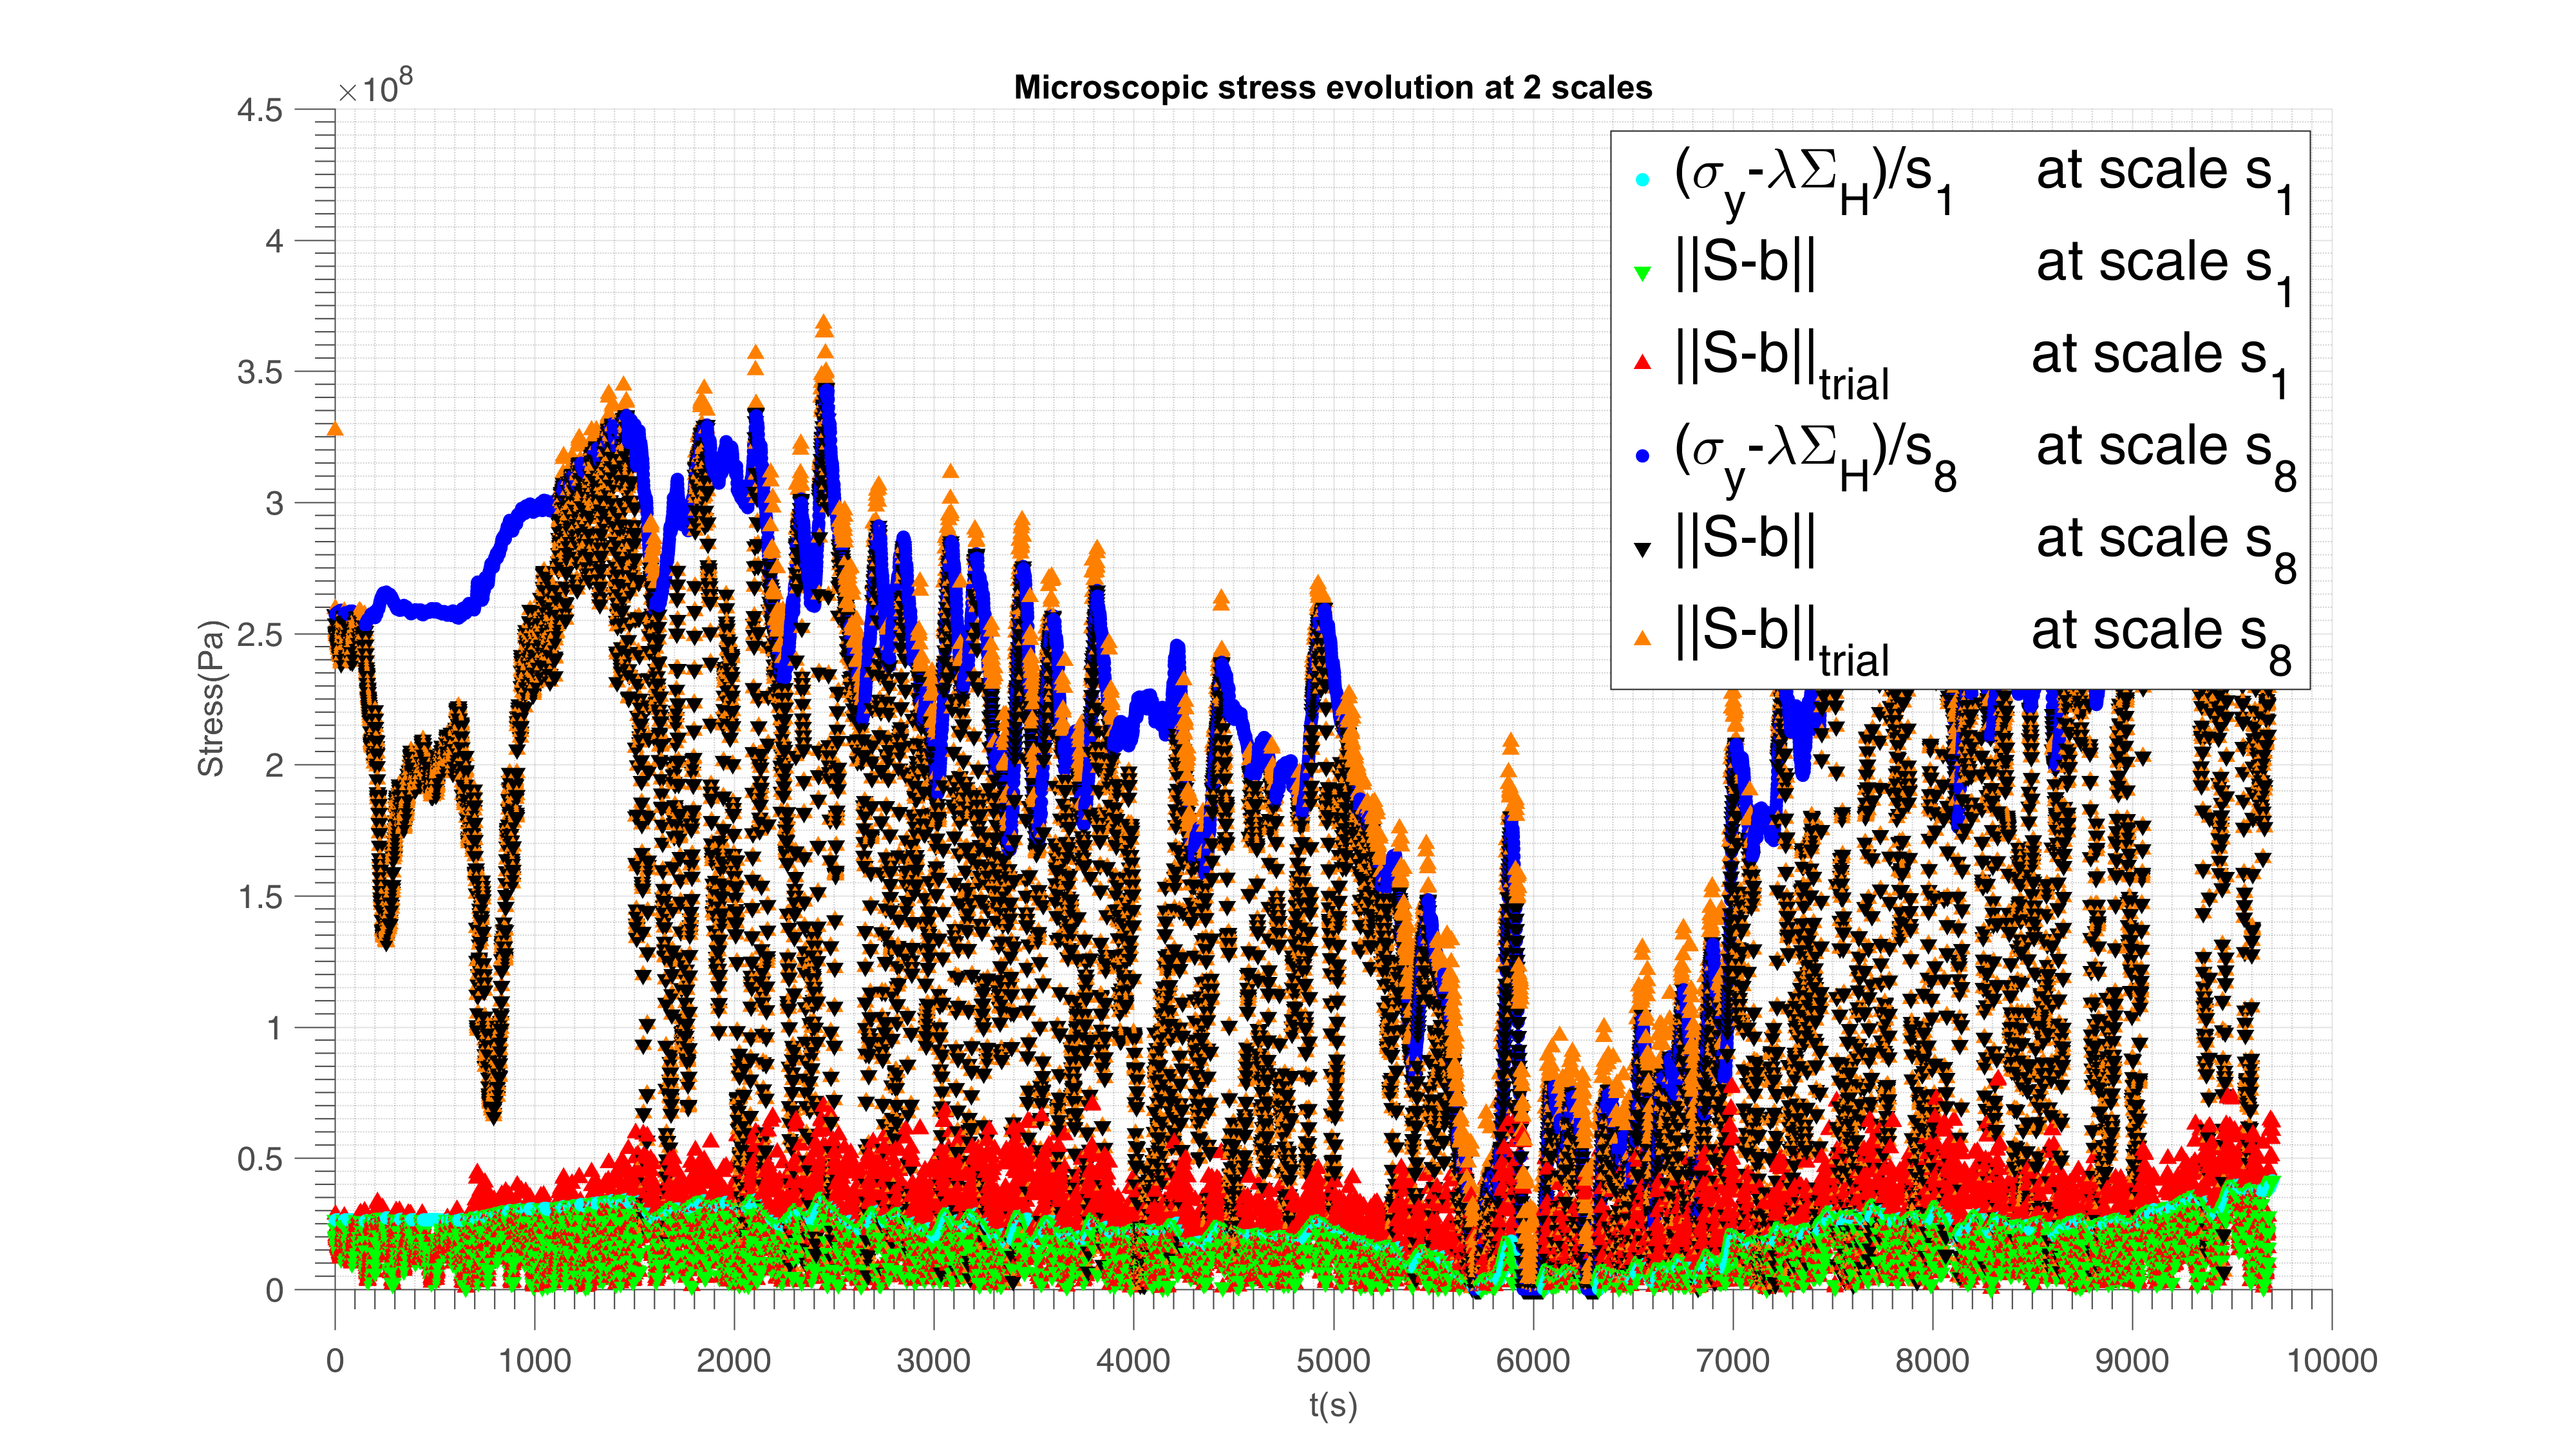
\includegraphics[width=\textwidth]{figures//trialreal3d.png} 
	\caption{$\left\|  \uline{\uline{S}}-\uline{\uline{b}}\right\|_{trial}$ and $\left\|  \uline{\uline{S}}-\uline{\uline{b}}\right\|$ evolution with time under different weakening scales in PSA load history}
	\label{trialreal3d}
\end{figure} 

In the load history, when $\left\|  \uline{\uline{S}}-\uline{\uline{b}}\right\|_{trial}>\left(\sigma_y-\lambda \Sigma_H\right)$, the damage accumulates. However, at scale $s_{8}$, there are much less damage accumulation than at scale $s_1$.  In this way we do not neglect the small influences in load history and the big fluctuation in stress is magnified which reflects the real situation. 


The damage evolves like in \figref{dam3d}. 


\begin{figure}[!h]
	\centering
	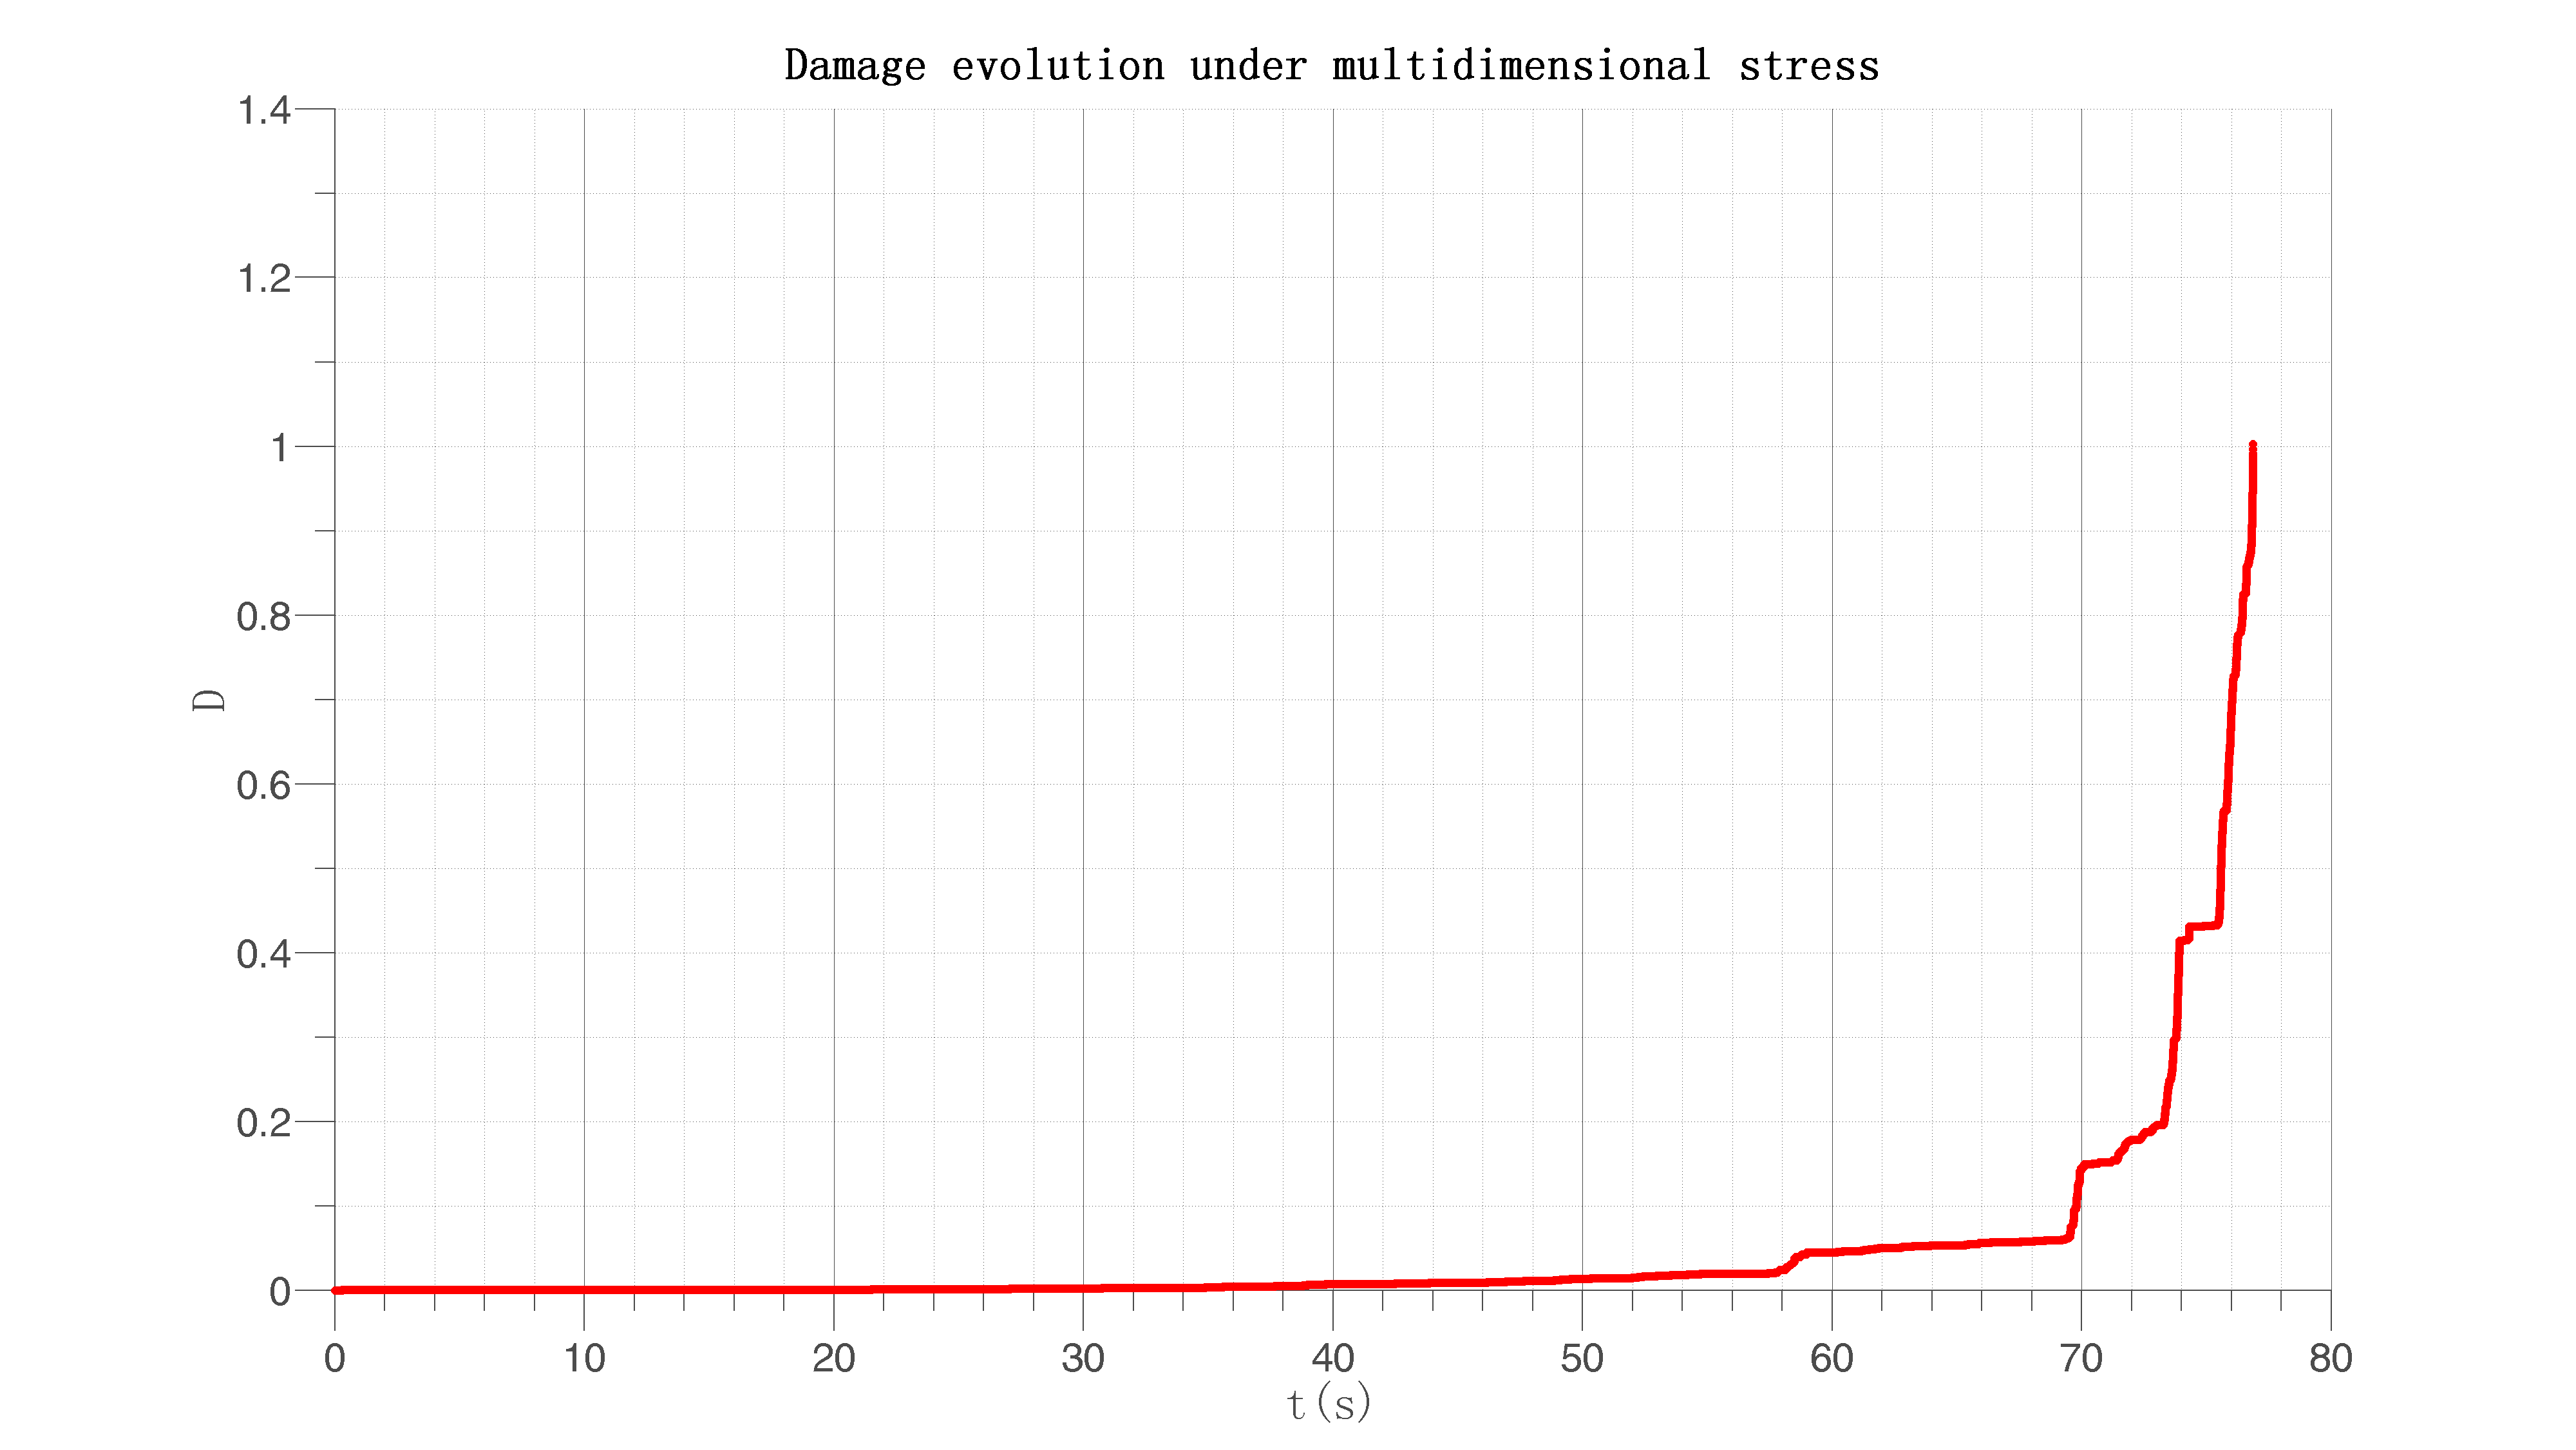
\includegraphics[width=\textwidth]{figures//damage3d.png} 
	\caption{Damage evolution under multidimensional stress}
	\label{dam3d}
\end{figure}

\end{comment}

\clearpage
\section{Discussion}
We work on the stress tensor directly in 3D analysis in stead of using the multidimensional equivalent stress.
The strategy can be made more complex by introducing a local space averaging process in the calculation of the local damage, and by taking more general plastic flows. The energy based fatigue approach takes into account impurities and hardness in the material and is applicable to any type of micro plasticity law and multiaxial load geometry. The time implicit strategy gets rid of cycle counting which is hardly applicable to complex loading, big fluctuation is magnified which reflects the real situation.

Further research of energy based failure criteria should be focused on the following aspects:
\begin{enumerate}
\item The accommodation law might be more elaborate than kinematic hardening.

\vspace{6pt}
\item The differentiation of shear stress and normal stress effect on fatigue life should be clarified.

\vspace{6pt}
\item The non-linearity parameter $\alpha$ contains the stress $\sigma$, so it can evolve with time. But for complex loading history, it should change at every time step.

\end{enumerate}

\vspace{6pt}
\noindent
\textbf{Acknowledgments}

\vspace{6pt}
We are grateful for the financial and technical support of Chaire PSA.

\bibliographystyle{unsrt}
\bibliography{11}
\addcontentsline{toc}{section}{Reference}



\clearpage
\appendix
\appendixpage
\addcontentsline{toc}{section}{Appendices}\markboth{APPENDICES}{}
\lstset{% general command to set parameter(s)
	basicstyle=\small, % 设置字体大小
	keywordstyle=\color{red}, % 设置关键字格式(颜色等等)
	identifierstyle=, % nothing happens
	commentstyle=\color{blue}, % 设置注释的格式
	stringstyle=\ttfamily, % typewriter type for strings
	showstringspaces=false} % no special string spaces
	\section{DETAILED EXPLOITATION}
	************************************************************************************

 A DETAILED DESCRIPTION OF ANALYTICAL EXPLOITATION ON UNIAXIAL CYCLE
 
\noindent              
************************************************************************************

\noindent
\textbf{Phase 1:} The deviatoric stress amplitude increases from $\sigma_y/s$ to $S_{max}$.

\noindent
The material is in local plastic regime, then $\dot{\varepsilon}^p>0$ and $\dot{\sigma}-\dot{b}=0$ $\Rightarrow$ $\dot{\Sigma}-\dfrac{E}{1+\nu}\dot{\varepsilon}^p=\dfrac{kE}{E-k}\dot{\varepsilon}^p$ $\Rightarrow$ 
$$\dot{\varepsilon}^p=\dfrac{(E- k)(1+\nu)}{E(E+k\nu)}\dot{\Sigma}.$$

\vspace{6pt}
\noindent
$\Rightarrow$ $\dot{\varepsilon}^p$ varies from 0 to $\dfrac{(E- k)(1+\nu)(S_{max}-\sigma_y/s)}{E(E+k\nu)}$.

\vspace{6pt}
\noindent
From Taylor-Lin scale transition model:
$$\dot{\sigma}=\dot{\Sigma}-\dfrac{E}{1+\nu}\dot{\varepsilon}_p=\dot{\Sigma}-\dfrac{E-k}{E-\nu k}\dot{\Sigma}=\dfrac{k(1-\nu)}{E-k\nu}\dot{\Sigma}.$$

\vspace{6pt}
\noindent
$\Rightarrow$ $\sigma$ varies from $\sigma_y/s$ to $\sigma_y/s+\dfrac{k(1-\nu)(S_{max}-\sigma_y/s)}{E-k\nu}$.

\vspace{6pt}
$$\dot{b}=\dot{\Sigma}-\dfrac{E}{1+\nu}\dot{\varepsilon}_p=\dot{\Sigma}-\dfrac{E-k}{E-\nu k}\dot{\Sigma}=\dfrac{k(1-\nu)}{E-k\nu}\dot{\Sigma}.$$

\vspace{6pt}
\noindent
$\Rightarrow$ $b$ varies from $0$ to $\dfrac{k(1-\nu)(S_{max}-\sigma_y/s)}{E-k\nu}$.

\vspace{6pt}
\noindent
So the energy dissipation rate is: $$(\sigma-b)\dot{\varepsilon}^p=\dfrac{\sigma_y}{s}\dot{\varepsilon}^p=\dfrac{\sigma_y}{s}\dfrac{(E- k)(1+\nu)}{E(E+k\nu)}\dot{\Sigma}.$$

\noindent
The energy dissipation is: $$(\sigma-b)\Delta\varepsilon^p=\dfrac{\sigma_y}{s}\dfrac{(E- k)(1+\nu)(S_{max}-\sigma_y/s)}{E(E+k\nu)}.$$

\vspace{6pt}
\noindent
\textbf{Phase 2:} The deviatoric stress amplitude decreases from $S_{max}$ to $S_{max}-2\sigma_y/s$.

\noindent
The material is in local elastic regime, then $\dot{\varepsilon}^p=0$ and $\dot{\sigma}-\dot{b}=0$ $\Rightarrow$

\vspace{6pt}
\noindent
$\dot{b}=0$, $\dot{\sigma}=\dot{\Sigma}-\dfrac{E}{1+\nu}\dot{\varepsilon}_p=\dot{\Sigma}$.

\vspace{6pt}
\noindent
$\sigma$ varies from $\sigma_y/s+\dfrac{k(1-\nu)(S_{max}-\sigma_y/s)}{E-k\nu}$ to $-\sigma_y/s+\dfrac{k(1-\nu)(S_{max}-\sigma_y/s)}{E-k\nu}$.

\vspace{6pt}
\noindent
$\sigma-b$ varies from $\sigma_y/s$ to $-\sigma_y/s$.

\vspace{6pt}
\noindent
The energy dissipation rate is: $$(\sigma-b)\dot{\varepsilon}^p=0.$$

\vspace{6pt}
\noindent
\textbf{Phase 3:} The deviatoric stress amplitude decreases from $S_{max}-2\sigma_y/s$ to $-S_{max}$.

\noindent
The material is in local plastic regime, then $\dot{\varepsilon}^p>0$ and $\dot{\sigma}-\dot{b}=0$ $\Rightarrow$ 
$$\dot{\varepsilon}^p=\dfrac{(E- k)(1+\nu)}{E(E+k\nu)}\dot{\Sigma}$$ as opposite to phase 1 for $\dot{\Sigma}<0$.

\vspace{6pt}
\noindent
$\Rightarrow$ $\varepsilon^p$ varies from $\dfrac{(E- k)(1+\nu)(S_{max}-\sigma_y/s)}{E(E+k\nu)}$ to 

\noindent
$\dfrac{(E- k)(1+\nu)(S_{max}-\sigma_y/s-S_{max}-(S_{max}-2\sigma_y/s))}{E(E+k\nu)}=-\dfrac{(E- k)(1+\nu)(S_{max}-\sigma_y/s)}{E(E+k\nu)}$.

\vspace{6pt}
\noindent
From Taylor-Lin scale transition model:
$$\dot{\sigma}=\dot{\Sigma}-\dfrac{E}{1+\nu}\dot{\varepsilon}_p=\dot{\Sigma}-\dfrac{E-k}{E-\nu k}\dot{\Sigma}=\dfrac{k(1-\nu)}{E-k\nu}\dot{\Sigma}.$$

\vspace{6pt}
\noindent
$\Rightarrow$ $\sigma$ varies from $-\sigma_y/s+\dfrac{k(1-\nu)(S_{max}-\sigma_y/s)}{E-k\nu}$ to $-\sigma_y/s-\dfrac{k(1-\nu)(S_{max}-\sigma_y/s)}{E-k\nu}$.

\vspace{6pt}
$$\dot{b}=\dot{\Sigma}-\dfrac{E}{1+\nu}\dot{\varepsilon}_p=\dot{\Sigma}-\dfrac{E-k}{E-\nu k}\dot{\Sigma}=\dfrac{k(1-\nu)}{E-k\nu}\dot{\Sigma}.$$
\vspace{6pt}
\noindent
$\Rightarrow$ $b$ varies from $\dfrac{k(1-\nu)(S_{max}-\sigma_y/s)}{E-k\nu}$ to $-\dfrac{k(1-\nu)(S_{max}-\sigma_y/s)}{E-k\nu}$.

\vspace{6pt}
\noindent
So the energy dissipation rate is: $$(\sigma-b)\dot{\varepsilon}^p=-\dfrac{\sigma_y}{s}\dot{\varepsilon}^p=-\dfrac{\sigma_y}{s}\dfrac{(E- k)(1+\nu)}{E(E+k\nu)}\dot{\Sigma}.$$

\noindent
The energy dissipation is: $$(\sigma-b)\Delta\varepsilon^p=-\dfrac{\sigma_y}{s}\dfrac{(E- k)(1+\nu)(-2S_{max}+2\sigma_y/s)}{E(E+k\nu)}=\dfrac{2\sigma_y}{s}\dfrac{(E- k)(1+\nu)(S_{max}-\sigma_y/s)}{E(E+k\nu)}.$$



\vspace{6pt}
\noindent
\textbf{Phase 4:} The deviatoric stress amplitude increases from $-S_{max}$ to $-S_{max}+2\sigma_y/s$.

\noindent
The material is in local elastic regime, then $\dot{\varepsilon}^p=0$ and $\dot{\sigma}-\dot{b}=0$ $\Rightarrow$

\vspace{6pt}
\noindent
$\dot{b}=0$, $\dot{\sigma}=\dot{\Sigma}-\dfrac{E}{1+\nu}\dot{\varepsilon}_p=\dot{\Sigma}$.

\vspace{6pt}
\noindent
$\sigma$ varies from $-\sigma_y/s-\dfrac{k(1-\nu)(S_{max}-\sigma_y/s)}{E-k\nu}$ to $\sigma_y/s-\dfrac{k(1-\nu)(S_{max}-\sigma_y/s)}{E-k\nu}$.

\vspace{6pt}
\noindent
$\sigma-b$ varies from $-\sigma_y/s$ to $\sigma_y/s$.

\vspace{6pt}
\noindent
So the energy dissipation rate is: $$(\sigma-b)\dot{\varepsilon}^p=0.$$


\vspace{6pt}
\noindent
\textbf{Phase 5:} The deviatoric stress amplitude increases from $-S_{max}+2\sigma_y/s$ to $\sigma_y/s$.

\noindent
The material is in local plastic regime, then $\dot{\varepsilon}^p>0$ and $\dot{\sigma}-\dot{b}=0$ $\Rightarrow$ 
$$\dot{\varepsilon}^p=\dfrac{(E- k)(1+\nu)}{E(E+k\nu)}\dot{\Sigma}$$ as in phase 1.

\vspace{6pt}
\noindent
$\Rightarrow$ $\dot{\varepsilon}^p$ varies from $-\dfrac{(E- k)(1+\nu)(S_{max}-\sigma_y/s)}{E(E+k\nu)}$ to $0$.

\vspace{6pt}
$$\dot{\sigma}=\dot{\Sigma}-\dfrac{E}{1+\nu}\dot{\varepsilon}_p=\dot{\Sigma}-\dfrac{E-k}{E-\nu k}\dot{\Sigma}=\dfrac{k(1-\nu)}{E-k\nu}\dot{\Sigma}.$$

\vspace{6pt}
\noindent
$\Rightarrow$ $\sigma$ varies from $\sigma_y/s-\dfrac{k(1-\nu)(S_{max}-\sigma_y/s)}{E-k\nu}$ to $\sigma_y/s$.

\vspace{6pt}
$$\dot{b}=\dot{\Sigma}-\dfrac{E}{1+\nu}\dot{\varepsilon}_p=\dot{\Sigma}-\dfrac{E-k}{E-\nu k}\dot{\Sigma}=\dfrac{k(1-\nu)}{E-k\nu}\dot{\Sigma}.$$
\vspace{6pt}
\noindent
$\Rightarrow$ $b$ varies from $-\dfrac{k(1-\nu)(S_{max}-\sigma_y/s)}{E-k\nu}$ to $0$.

\vspace{6pt}
\noindent
So the energy dissipation rate is: $$(\sigma-b)\dot{\varepsilon}^p=\dfrac{\sigma_y}{s}\dot{\varepsilon}^p=\dfrac{\sigma_y}{s}\dfrac{(E- k)(1+\nu)}{E(E+k\nu)}\dot{\Sigma}.$$

\noindent
The energy dissipation is: $$(\sigma-b)\Delta\varepsilon^p=\dfrac{\sigma_y}{s}\dfrac{(E- k)(1+\nu)(S_{max}-\sigma_y/s)}{E(E+k\nu)}.$$


From the three phase analysis in local plastic regime, the dissipated energy is like $dW(phase1)=\dfrac{1}{2}dW(phase3)=dW(phase5)$ and the dissipation rate is like $d\dot{W}(phase1)=d\dot{W}(phase3)=d\dot{W}(phase5)$.
\begin{equation}d\dot{W}=\dfrac{(E-k)(1+\nu) }{E(E-k\nu)}\left( \dfrac{\sigma_y}{s}\right) \left| \dot{\Sigma}\right|   
\end{equation}


	\clearpage
************************************************************************************

MULTI-DIMENSIONAL PLASTIC AND ELASTIC REGIME ANALYSIS

************************************************************************************

At a certain scale $s_i$, after elimination of $ \dot{\uline{\uline{\varepsilon}}}^p$, there are 
$$\dot{\uline{\uline{S}}}- \dot{\uline{\uline{b}}}= dev\dot{\uline{\uline{\Sigma}}}-E\gamma\left( \dfrac{1}{1+\nu}+\dfrac{k}{E-k}\right)\dfrac{\uline{\uline{S}}-\uline{\uline{b}}}{\left| \left|\uline{\uline{S}}-\uline{\uline{b}}\right| \right|}. $$

If we are at yield limit at (t+dt), we get on the other hand:
$$\left( \uline{\uline{S}}-\uline{\uline{b}}\right) (t+dt)=\left( \uline{\uline{S}}-\uline{\uline{b}}\right) (t)+\left( \dot{\uline{\uline{S}}}- \dot{\uline{\uline{b}}}\right) dt,$$
\begin{equation}\left| \left| \left( \uline{\uline{S}}-\uline{\uline{b}}\right) (t+dt)\right| \right| =\left( \sigma_y-\lambda \sigma_m\right)/s_i .
\end{equation}

Replacing $\left( \dot{\uline{\uline{S}}}-\dot{\uline{\uline{b}}}\right) $ in the integration by its expression we get:
\begin{equation}
\left( \uline{\uline{S}}-\uline{\uline{b}}\right) (t+dt)=\left( \uline{\uline{S}}-\uline{\uline{b}}\right) (t)+dev\dot{\uline{\uline{\Sigma}}}dt-E\gamma dt\left(\dfrac{1}{1+\nu}+\dfrac{k}{E-k} \right) \dfrac{\left( \uline{\uline{S}}-\uline{\uline{b}}\right) (t+dt)}{\left| \left|\uline{\uline{S}}-\uline{\uline{b}}\right| \right| (t+dt)}
\end{equation}

Putting all terms with $ \left( \uline{\uline{S}}-\uline{\uline{b}}\right) (t+dt)$ on the left hand side, we get:
\begin{equation}
\left( \uline{\uline{S}}-\uline{\uline{b}}\right) (t+dt)\left(  1+\eta\right) =\left( \uline{\uline{S}}-\uline{\uline{b}}\right) (t)+dev\dot{\uline{\uline{\Sigma}}}dt=\left( \uline{\uline{S}}-\uline{\uline{b}}\right)_{trial} (t+dt)
\label{eqyield}
\end{equation}
with\begin{equation}\eta=\dfrac{E\gamma dt}{\left| \left|\uline{\uline{S}}-\uline{\uline{b}}\right| \right|(t+dt)}\left(\dfrac{1}{1+\nu}+\dfrac{k}{E-k} \right).
\label{eta}
\end{equation}

To see whether the structure is in elastic or plastic regime at each time step, we use $\left( \uline{\uline{S}}-\uline{\uline{b}}\right)_{trial}(t+dt)$ to compare with the yield stress at the same scale $s_i$, thus to give a value to $\left( \uline{\uline{S}}-\uline{\uline{b}}\right)(t+dt)$.

Since $\left( \uline{\uline{S}}-\uline{\uline{b}}\right)(t+dt)$ is in the same direction as $\left( \uline{\uline{S}}-\uline{\uline{b}}\right)_{trial}(t+dt)$, we have
\begin{equation}\left( \uline{\uline{S}}-\uline{\uline{b}}\right) (t+dt)= \left( \sigma_y-\lambda \sigma_H(t+dt)\right)/s\dfrac{\left( \uline{\uline{S}}-\uline{\uline{b}}\right)_{trial}(t+dt)}{\left| \left|\uline{\uline{S}}-\uline{\uline{b}}\right| \right|_{trial}(t+dt)}
\label{eqdirection}\end{equation}

We now compare Eq.\eqref{eqyield} and Eq.\eqref{eqdirection}, the only solution is to have:

\begin{equation}
1+\eta=\dfrac{\left| \left|\uline{\uline{S}}-\uline{\uline{b}}\right| \right|_{trial}}{\left( \sigma_y-\lambda \sigma_m\right)/s}
\end{equation}
that is:
\begin{equation}
\eta=\dfrac{\left| \left|\uline{\uline{S}}-\uline{\uline{b}}\right| \right|_{trial}}{\left( \sigma_y-\lambda \sigma_m\right)/s}-1
\label{eta2}
\end{equation}
which is positive in plastic regime.



\end{document}


